% LaTeX support: latex@mdpi.com
% For support, please attach all files needed for compiling as well as the log file, and specify your operating system, LaTeX version, and LaTeX editor.

%=================================================================
\documentclass[metals,article,accept,pdftex,moreauthors]{Definitions/mdpi}
% For posting an early version of this manuscript as a preprint, you may use "preprints" as the journal and change "submit" to "accept". The document class line would be, e.g., \documentclass[preprints,article,accept,moreauthors,pdftex]{mdpi}. This is especially recommended for submission to arXiv, where line numbers should be removed before posting. For preprints.org, the editorial staff will make this change immediately prior to posting.

%--------------------
% Class Options:
%--------------------
%----------
% journal
%----------
% Choose between the following MDPI journals:
% acoustics, actuators, addictions, admsci, adolescents, aerobiology, aerospace, agriculture, agriengineering, agrochemicals, agronomy, ai, air, algorithms, allergies, alloys, analytica, analytics, anatomia, animals, antibiotics, antibodies, antioxidants, applbiosci, appliedchem, appliedmath, applmech, applmicrobiol, applnano, applsci, aquacj, architecture, arm, arthropoda, arts, asc, asi, astronomy, atmosphere, atoms, audiolres, automation, axioms, bacteria, batteries, bdcc, behavsci, beverages, biochem, bioengineering, biologics, biology, biomass, biomechanics, biomed, biomedicines, biomedinformatics, biomimetics, biomolecules, biophysica, biosensors, biotech, birds, bloods, blsf, brainsci, breath, buildings, businesses, cancers, carbon, cardiogenetics, catalysts, cells, ceramics, challenges, chemengineering, chemistry, chemosensors, chemproc, children, chips, cimb, civileng, cleantechnol, climate, clinpract, clockssleep, cmd, coasts, coatings, colloids, colorants, commodities, compounds, computation, computers, condensedmatter, conservation, constrmater, cosmetics, covid, crops, cryptography, crystals, csmf, ctn, curroncol, cyber, dairy, data, ddc, dentistry, dermato, dermatopathology, designs, devices, diabetology, diagnostics, dietetics, digital, disabilities, diseases, diversity, dna, drones, dynamics, earth, ebj, ecologies, econometrics, economies, education, ejihpe, electricity, electrochem, electronicmat, electronics, encyclopedia, endocrines, energies, eng, engproc, entomology, entropy, environments, environsciproc, epidemiologia, epigenomes, est, fermentation, fibers, fintech, fire, fishes, fluids, foods, forecasting, forensicsci, forests, foundations, fractalfract, fuels, future, futureinternet, futurepharmacol, futurephys, futuretransp, galaxies, games, gases, gastroent, gastrointestdisord, gels, genealogy, genes, geographies, geohazards, geomatics, geosciences, geotechnics, geriatrics, grasses, gucdd, hazardousmatters, healthcare, hearts, hemato, hematolrep, heritage, higheredu, highthroughput, histories, horticulturae, hospitals, humanities, humans, hydrobiology, hydrogen, hydrology, hygiene, idr, ijerph, ijfs, ijgi, ijms, ijns, ijpb, ijtm, ijtpp, ime, immuno, informatics, information, infrastructures, inorganics, insects, instruments, inventions, iot, j, jal, jcdd, jcm, jcp, jcs, jcto, jdb, jeta, jfb, jfmk, jimaging, jintelligence, jlpea, jmmp, jmp, jmse, jne, jnt, jof, joitmc, jor, journalmedia, jox, jpm, jrfm, jsan, jtaer, jvd, jzbg, kidneydial, kinasesphosphatases, knowledge, land, languages, laws, life, liquids, literature, livers, logics, logistics, lubricants, lymphatics, machines, macromol, magnetism, magnetochemistry, make, marinedrugs, materials, materproc, mathematics, mca, measurements, medicina, medicines, medsci, membranes, merits, metabolites, metals, meteorology, methane, metrology, micro, microarrays, microbiolres, micromachines, microorganisms, microplastics, minerals, mining, modelling, molbank, molecules, mps, msf, mti, muscles, nanoenergyadv, nanomanufacturing,\gdef\@continuouspages{yes}} nanomaterials, ncrna, ndt, network, neuroglia, neurolint, neurosci, nitrogen, notspecified, %%nri, nursrep, nutraceuticals, nutrients, obesities, oceans, ohbm, onco, %oncopathology, optics, oral, organics, organoids, osteology, oxygen, parasites, parasitologia, particles, pathogens, pathophysiology, pediatrrep, pharmaceuticals, pharmaceutics, pharmacoepidemiology,\gdef\@ISSN{2813-0618}\gdef\@continuous pharmacy, philosophies, photochem, photonics, phycology, physchem, physics, physiologia, plants, plasma, platforms, pollutants, polymers, polysaccharides, poultry, powders, preprints, proceedings, processes, prosthesis, proteomes, psf, psych, psychiatryint, psychoactives, publications, quantumrep, quaternary, qubs, radiation, reactions, receptors, recycling, regeneration, religions, remotesensing, reports, reprodmed, resources, rheumato, risks, robotics, ruminants, safety, sci, scipharm, sclerosis, seeds, sensors, separations, sexes, signals, sinusitis, skins, smartcities, sna, societies, socsci, software, soilsystems, solar, solids, spectroscj, sports, standards, stats, std, stresses, surfaces, surgeries, suschem, sustainability, symmetry, synbio, systems, targets, taxonomy, technologies, telecom, test, textiles, thalassrep, thermo, tomography, tourismhosp, toxics, toxins, transplantology, transportation, traumacare, traumas, tropicalmed, universe, urbansci, uro, vaccines, vehicles, venereology, vetsci, vibration, virtualworlds, viruses, vision, waste, water, wem, wevj, wind, women, world, youth, zoonoticdis
% For posting an early version of this manuscript as a preprint, you may use "preprints" as the journal. Changing "submit" to "accept" before posting will remove line numbers.

%---------
% article
%---------
% The default type of manuscript is "article", but can be replaced by:
% abstract, addendum, article, book, bookreview, briefreport, casereport, comment, commentary, communication, conferenceproceedings, correction, conferencereport, entry, expressionofconcern, extendedabstract, datadescriptor, editorial, essay, erratum, hypothesis, interestingimage, obituary, opinion, projectreport, reply, retraction, review, perspective, protocol, shortnote, studyprotocol, systematicreview, supfile, technicalnote, viewpoint, guidelines, registeredreport, tutorial
% supfile = supplementary materials

%----------
% submit
%----------
% The class option "submit" will be changed to "accept" by the Editorial Office when the paper is accepted. This will only make changes to the frontpage (e.g., the logo of the journal will get visible), the headings, and the copyright information. Also, line numbering will be removed. Journal info and pagination for accepted papers will also be assigned by the Editorial Office.

%------------------
% moreauthors
%------------------
% If there is only one author the class option oneauthor should be used. Otherwise use the class option moreauthors.

%---------
% pdftex
%---------
% The option pdftex is for use with pdfLaTeX. Remove "pdftex" for (1) compiling with LaTeX & dvi2pdf (if eps figures are used) or for (2) compiling with XeLaTeX.

%=================================================================
% MDPI internal commands - do not modify
% MDPI internal commands - do not modify
\firstpage{1}
\makeatletter
\setcounter{page}{\@firstpage}
\makeatother
\pubvolume{13}
\issuenum{3}
\articlenumber{633}
\pubyear{2023}
\copyrightyear{2023}
\externaleditor{Academic Editor: {Ji Hoon Kim} %MDPI: Please add it.
}
\datereceived{ 10 February 2023}
\daterevised{ 16 March 2023} % Comment out if no revised date
\dateaccepted{20 March 2023}
\datepublished{22 March 2023}
%\datecorrected{} % For corrected papers: "Corrected: XXX" date in the original paper.
%\dateretracted{} % For corrected papers: "Retracted: XXX" date in the original paper.
\hreflink{https://doi.org/10.3390/\linebreak met13030633} % If needed use \linebreak
%\doinum{}
%\pdfoutput=1 % Uncommented for upload to arXiv.org

%=================================================================
% Add packages and commands here. The following packages are loaded in our class file: fontenc, inputenc, calc, indentfirst, fancyhdr, graphicx, epstopdf, lastpage, ifthen, float, amsmath, amssymb, lineno, setspace, enumitem, mathpazo, booktabs, titlesec, etoolbox, tabto, xcolor, colortbl, soul, multirow, microtype, tikz, totcount, changepage, attrib, upgreek, array, tabularx, pbox, ragged2e, tocloft, marginnote, marginfix, enotez, amsthm, natbib, hyperref, cleveref, scrextend, url, geometry, newfloat, caption, draftwatermark, seqsplit
% cleveref: load \crefname definitions after \begin{document}

\usepackage{gensymb}
\usepackage{accents}
\usepackage{xspace}
\usepackage[labelformat=simple]{subcaption}
\renewcommand\thesubfigure{\alph{subfigure}}
\DeclareCaptionLabelFormat{subcaptionlabel}{\normalfont(\textbf{#2}\normalfont)}
\captionsetup[subfigure]{labelformat=subcaptionlabel}

\DeclareRobustCommand{\w}{\mbox{\large\ensuremath{\mathsf{w}}}}
\DeclareRobustCommand{\dotp}{\boldsymbol{\cdot}}
\DeclareRobustCommand{\e}[1]{{\rm e}^{#1}}
\DeclareRobustCommand{\lay}[1]{^{(#1)}}
\DeclareRobustCommand{\mdot}[1]{\accentset{\mbox{\bfseries .}}{#1}}
\DeclareRobustCommand{\ie}{i.e.,\@\xspace}
\DeclareRobustCommand{\eal}{et al.\@\xspace}
\DeclareRobustCommand{\eg}{e.g.,\@\xspace}
\DeclareRobustCommand{\RMSE}{\text{E}_\text{RMS}}
\DeclareRobustCommand{\MARE}{\text{E}_\text{MAR}}
\DeclareRobustCommand{\R}{\text{R}}
\DeclareRobustCommand{\ps}{\text{s}^{-1}}
\DeclareRobustCommand{\mr}[2]{\multirow{#1}{*}{#2}}
\DeclareRobustCommand{\MPa}{\text{MPa}}
\newcommand{\hlok}[1]{\colorbox{green}{#1}}

%=================================================================
% Please use the following mathematics environments: Theorem, Lemma, Corollary, Proposition, Characterization, Property, Problem, Example, ExamplesandDefinitions, Hypothesis, Remark, Definition, Notation, Assumption
%% For proofs, please use the proof environment (the amsthm package is loaded by the MDPI class).

%=================================================================
% Full title of the paper (Capitalized)
\Title{Interpolation and Extrapolation Performance Measurement of Analytical and ANN-Based Flow Laws for Hot Deformation Behavior of Medium Carbon Steel}

% MDPI internal command: Title for citation in the left column
\TitleCitation{Interpolation and Extrapolation Performance Measurement of Analytical and ANN-Based Flow Laws for Hot Deformation Behavior of Medium Carbon Steel}

% Author Orchid ID: enter ID or remove command
\newcommand{\orcidauthorA}{0000-0001-7367-5453} % Add \orcidA{} behind the author's name
\newcommand{\orcidauthorB}{0000-0002-1522-2787} % Add \orcidB{} behind the author's name
\newcommand{\orcidauthorC}{0000-0002-5360-5121}
\newcommand{\orcidauthorD}{0000-0002-0815-1984}

% Authors, for the paper (add full first names)
\Author{{Pierre Tize Mha} %Please carefully check the accuracy of names and affiliations. Changes will not be possible after proofreading. All names are correct
$^{1}$\orcidD{}, Prashant Dhondapure $^{2}$, Mohammad Jahazi $^{2}$\orcidB{}, Amèvi Tongne $^{1}$\orcidC{} and Olivier Pantalé $^{1,}$*\orcidA{}}

%\longauthorlist{yes}

% MDPI internal command: Authors, for metadata in PDF
\AuthorNames{Pierre Tize Mha, Prashant Dhondapure, Mohammad Jahazi, Amèvi Tongne, Olivier Pantalé}

% MDPI internal command: Authors, for citation in the left column
\AuthorCitation{Tize Mha, P.; Dhondapure, P.; Jahazi, M.; Tongne, A.; Pantalé, O.}
% If this is a Chicago style journal: Lastname, Firstname, Firstname Lastname, and Firstname Lastname.

% Affiliations / Addresses (Add [1] after \address if there is only one affiliation.)
\address{$^{1}$ \quad Laboratoire Génie de Production, INP/ENIT, Université de Toulouse, 47 Av d'Azereix, F-65016 Tarbes, France; {ptizemha@enit.fr (P.T.M.); amevi.tongne@enit.fr (A.T.)} %MDPI: We added emails from our system. Please confirm. OK
\\
$^{2}$ \quad Department of Mechanical Engineering, École de Technologie Supérieure, 1100 Notre Dame St. W., \mbox{Montréal, QC H3C 1K3, Canada}; prashant-nagnath.dhondapure.1@ens.etsmtl.ca (P.D.); \mbox{mohammad.jahazi@etsmtl.ca (M.J.)}}

% Contact information of the corresponding author
\corres{Correspondence: olivier.pantale@enit.fr; Tel.: +33-562442933}

% Current address and/or shared authorship
%\firstnote{Current address: Affiliation 3.}
%\secondnote{These authors contributed equally to this work.}
% The commands \thirdnote{} till \eighthnote{} are available for further notes

%\simplesumm{} % Simple summary

%\conference{} % An extended version of a conference paper

% Abstract (Do not insert blank lines, i.e. \\)
\abstract{In the present work, a critical analysis of the most-commonly used analytical models and recently introduced ANN-based models was performed to evaluate their predictive accuracy within and outside the experimental interval used to generate them.
The high-temperature deformation behavior of a medium carbon steel was studied over a wide range of strains, strain rates, and temperatures using hot compression tests on a Gleeble-3800.
The experimental flow curves were modeled using the Johnson--Cook, Modified-Zerilli--Armstrong, Hansel--Spittel, Arrhenius, and PTM models, as well as an ANN model.
The mean absolute relative error and root-mean-squared error values were used to quantify the predictive accuracy of the models analyzed.
The results indicated that the Johnson--Cook and Modified-Zerilli--Armstrong models had a significant error, while the Hansel--Spittel, PTM, and Arrhenius models were able to predict the behavior of this alloy.
The ANN model showed excellent agreement between the predicted and experimental flow curves, with an error of less than 0.62\%.
To validate the performance, the ability to interpolate and extrapolate the experimental data was also tested.
The Hansel--Spittel, PTM, and Arrhenius models showed good interpolation and extrapolation capabilities.
However, the ANN model was the most-powerful of all the models.}

% Keywords
\keyword{{artificial} %mdpi: please check the first letter format (uppercase/lowercase) for every word in keywords. please check all the keywords. we suggest to use lowercase if the uppercase is not necessary: OK
neural network; constitutive flow law; analytical flow law; interpolation; \linebreak extrapolation; Gleeble}

% The fields PACS, MSC, and JEL may be left empty or commented out if not applicable
%\PACS{J0101}
%\MSC{}
%\JEL{}

%%%%%%%%%%%%%%%%%%%%%%%%%%%%%%%%%%%%%%%%%%
% Only for the journal Diversity
%\LSID{\url{http://}}

%%%%%%%%%%%%%%%%%%%%%%%%%%%%%%%%%%%%%%%%%%
% Only for the journal Applied Sciences
%\featuredapplication{Authors are encouraged to provide a concise description of the specific application or a potential application of the work. This section is not mandatory.}
%%%%%%%%%%%%%%%%%%%%%%%%%%%%%%%%%%%%%%%%%%

%%%%%%%%%%%%%%%%%%%%%%%%%%%%%%%%%%%%%%%%%%
% Only for the journal Data
%\dataset{DOI number or link to the deposited data set if the data set is published separately. If the data set shall be published as a supplement to this paper, this field will be filled by the journal editors. In this case, please submit the data set as a supplement.}
%\datasetlicense{License under which the data set is made available (CC0, CC-BY, CC-BY-SA, CC-BY-NC, etc.)}

%%%%%%%%%%%%%%%%%%%%%%%%%%%%%%%%%%%%%%%%%%
% Only for the journal Toxins
%\keycontribution{The breakthroughs or highlights of the manuscript. Authors can write one or two sentences to describe the most important part of the paper.}

%%%%%%%%%%%%%%%%%%%%%%%%%%%%%%%%%%%%%%%%%%
% Only for the journal Encyclopedia
%\encyclopediadef{For entry manuscripts only: please provide a brief overview of the entry title instead of an abstract.}

%%%%%%%%%%%%%%%%%%%%%%%%%%%%%%%%%%%%%%%%%%
% Only for the journal Advances in Respiratory Medicine
%\addhighlights{yes}
%\renewcommand{\addhighlights}{%

%\noindent This is an obligatory section in “Advances in Respiratory Medicine”, whose goal is to increase the discoverability and readability of the article via search engines and other scholars. Highlights should not be a copy of the abstract, but a simple text allowing the reader to quickly and simplified find out what the article is about and what can be cited from it. Each of these parts should be devoted up to 2~bullet points.\vspace{3pt}\\
%\textbf{What are the main findings?}
% \begin{itemize}[labelsep=2.5mm,topsep=-3pt]
% \item First bullet.
% \item Second bullet.
% \end{itemize}\vspace{3pt}
%\textbf{What is the implication of the main finding?}
% \begin{itemize}[labelsep=2.5mm,topsep=-3pt]
% \item First bullet.
% \item Second bullet.
% \end{itemize}
%}

%%%%%%%%%%%%%%%%%%%%%%%%%%%%%%%%%%%%%%%%%%
\begin{document}

%----------------------------------------------------------------------------------
\section{Introduction\label{sec:Introduction}}
%----------------------------------------------------------------------------------
Large size forged blocks made of medium carbon high-strength steels are extensively used in the automotive industry as dies for the production of bumpers and dashboards through the plastic injection process.
The manufacturing process of the large blocks starts with ingot casting, followed by open die forging and a quench and temper heat treatment process to achieve the desired mechanical properties \cite{chadha2017deformation, chadha2018influence, murugesan2019two}.
In recent years, in order to respond to the market demand, larger size forgings have had to be produced.
In parallel, more stringent conditions related to chemical homogeneity, hardness, grain size, and mechanical properties from the surface to the core of the forged block have been required.
Of the three manufacturing steps (casting, forging, and heat treatment), forging is where the most-important microstructural changes take place, which greatly influence the final properties that can be achieved \cite{murugesan2019hybrid, chadha2020microstructure, sripada2022effect}.
The open die forging process is fundamentally a hot compression process during which work strengthening effects, such as hardening (WH) and precipitation, take place concomitantly with softening phenomena such as recovery and recrystallization under static and/or dynamic thermomechanical loads~\cite{tian2022deformation, tavakoli2019ferrite}.
It has also been reported that phase transformation can occur during deformation.
The extent and intensity of the above phenomena strongly depend on three macroscopic quantities, namely the strain $\varepsilon$, the strain rate $\mdot\varepsilon$, and the temperature $T$ \cite{ebrahimi2017flow, shi2022constitutive, zeng2022constitutive, rudra2019constitutive}.

Considering the large size of blocks, a purely experimental approach, based on trial and error, cannot be used by industry, and therefore, reliable predictive tools, such a finite element analysis (FEA) codes, have been developed and are commercially available.
However, the prediction reliability of such analyses is a function of the accuracy of the material constitutive model, which describes the mutual interactions between the strain, the strain rate, and the temperature during deformation.
As mentioned above, precipitation and phase changes are considered negligible as deformation takes place in the austenite phase at temperatures above the dissolution temperature of most carbides.
Hence, most constitutive models depend on macroscopic parameters, which influence the hardening and softening of the material.
A large number of phenomenological, semi-empirical, or physical \mbox{models~\cite{jia2022thermo, costa2016study, rudnytskyj2020constitutive, Pantale-2021}} have been developed.
Among these, the Johnson--Cook (JC) \cite{Johnson-1983}, Hansel--Spittel (HS) \cite{chadha2018approach}, and Zerilli--Armstrong (ZA) \cite{Zerilli-1987} models are the best-known and most-widely available in FEA codes.
Despite their simplicity, each of them suffers from certain shortcomings: as reported by Jia \eal \cite{Jia-2021}, the JC model suffers from a lack of non-coupling between the strain, the strain rate, and the temperature, while the HS model is better adapted for higher strain rate conditions \cite{chadha2018approach}.
To circumvent these shortcomings, several modified model forms have been developed \cite{chadha2018approach, liu2021modified, jia2022thermo1, bai2022comparison, zhu2022constitutive, Jia-2021, sim2022modified}.
However, as reported by many authors \cite{Li-2013, Zhang-2015, Zhou-2019}, even after adjusting the constants, the high-temperature flow behavior, particularly when dynamic recrystallization takes place, cannot be accurately predicted, and none of the models is able to accurately predict the flow behavior outside the experimental testing interval that was used to determine the model constants.
Due to its more physics-based formulation, the ZA model and its modified form, MZA \cite{ovesy2020explicit, niu2020constitutive, Muralli-2017, Cheng-2021, Muralli-2021}, and the Arrhenius-type hyperbolic sine constitutive models are preferred to the JC and HS models both for the prediction of the hot deformation behavior and microstructure analysis of the material \cite{derazkola2021review, wang2022deformation, miao2022deformation}.
The Arrhenius formulation has been revised repeatedly to achieve a more accurate determination of the activation energy for high-temperature deformation \cite{rudnytskyj2022investigating, ji2020optimization}.
To overcome the strong dependency of the models on specific alloy types, Tize Mha \eal \cite{TizeMha-2022} recently proposed a constitutive model, PTM, whose formulation is independent of the alloy type.
This formulation is based on the MZA model and the polynomial functions of undefined order that are used during the identification.
However, in the PTM model, the high order of the polynomial function (up to $10$ in some cases) can affect its accuracy.

The artificial neural network (ANN) is an approach used to predict the flow stress behavior of materials without requiring a mathematical formulation of the flow law.
It is therefore not necessary to postulate a mathematical expression to identify the parameters of the model.
Since the behavior of materials is highly nonlinear at high temperatures and depends on many factors, which are also nonlinear, the evaluation of the flow stress behavior by an analytical model whose parameters are identified by a classical regression method is limited.
Faced with these limitations, ANN models are of major interest because they are particularly suited to dealing with complex and nonlinear relationships.
Consequently, ANNs have been successfully applied to predict the flow stress behavior of materials under hot working conditions \cite{wu2022experimental, stoffel2020deep, Ashtiani-2016-CSP, Stoffel-2019-NNB}.
Although ANN models can predict well the material flow behavior, there is a problem with their implementation in finite element software, as reported by Pantalé \eal \cite{Pantale-2021, Pantale-2023}.
In fact, the implementation of a constitutive model in an FEA code requires the derivatives of the model with respect to the strain, strain rate, and temperature.

Although progress has been made in improving constitutive models to better predict the flow stress behavior of materials, problems still persist with the models' efficiency.
Indeed, a model is considered appropriate for predicting the material's behavior if its predictions and experimental results correlate well.
It is questionable whether a model that correctly describes the behavior of a material in a defined experimental window can be used to accurately predict its behavior for conditions different from those for which it was identified.
In other words, the question is whether interpolation and extrapolation techniques can be used to extend the applicability of a constitutive equation for different processing windows.

The present work aimed to address the preceding question using the recently introduced ANN model.
To this end, initially, hot compression tests, simulating the open die forging process, were carried out, and the flow curves generated were modeled using the above-mentioned constitutive equations and an ANN model developed in this work.
Then, the interpolation and extrapolation capabilities of each model were evaluated.
The results were validated based on experimental work carried out herein and on data obtained from the~literature.

%----------------------------------------------------------------------------------
\section{Materials and Experiments\label{sec:Materials}}
%----------------------------------------------------------------------------------

%----------------------------------------------------------------------------------
\subsection{Experimental Procedure}
%----------------------------------------------------------------------------------

The material used in this study consisted of a medium carbon steel whose chemical composition is given in Table \ref{tab:Composition}.
\begin{table}[H]
\centering
\caption{Chemical composition of medium carbon steel. Fe = balance.}

\newcolumntype{L}{>{\raggedright\arraybackslash}X}
\newcolumntype{C}{>{\centering\arraybackslash}X}
\begin{tabularx}{\textwidth}{LCCCCCCC}
\toprule
\textbf{Element} & \textbf{C} & \textbf{Mn} & \textbf{Mo} & \textbf{Si} & \textbf{Ni} & \textbf{Cr} & \textbf{Cu} \\
\midrule
{{Wt}%MDPI: Is the bold necessary?. You can remove the bold, if it does not correspond to the editorial line of the journal.
~\%} & $0.30$ & $0.89$ & $0.52$ & $0.34$ & $0.68$ & $1.86$ & $0.17$ \\
\bottomrule
\end{tabularx}
\label{tab:Composition}
\end{table}
Cylindrical samples were machined with an initial diameter of $d=10$~mm and a height of $h_0=15$~mm.
Hot compression tests were performed on a Gleeble-3800 thermomechanical simulator (see Figure \ref{fig:Gleeble3800}), for $5$ temperature levels, namely $1050~\celsius$, $1100~\celsius$, $1150~\celsius$, $1200~\celsius$, and $1250~\celsius$, with the $6$ strain rates of $0.001~\ps$, $0.01~\ps$, $0.1~\ps$, $1~\ps$, $2.0~\ps$, and $5~\ps$.

\vspace{2pt}
\begin{figure}[H]

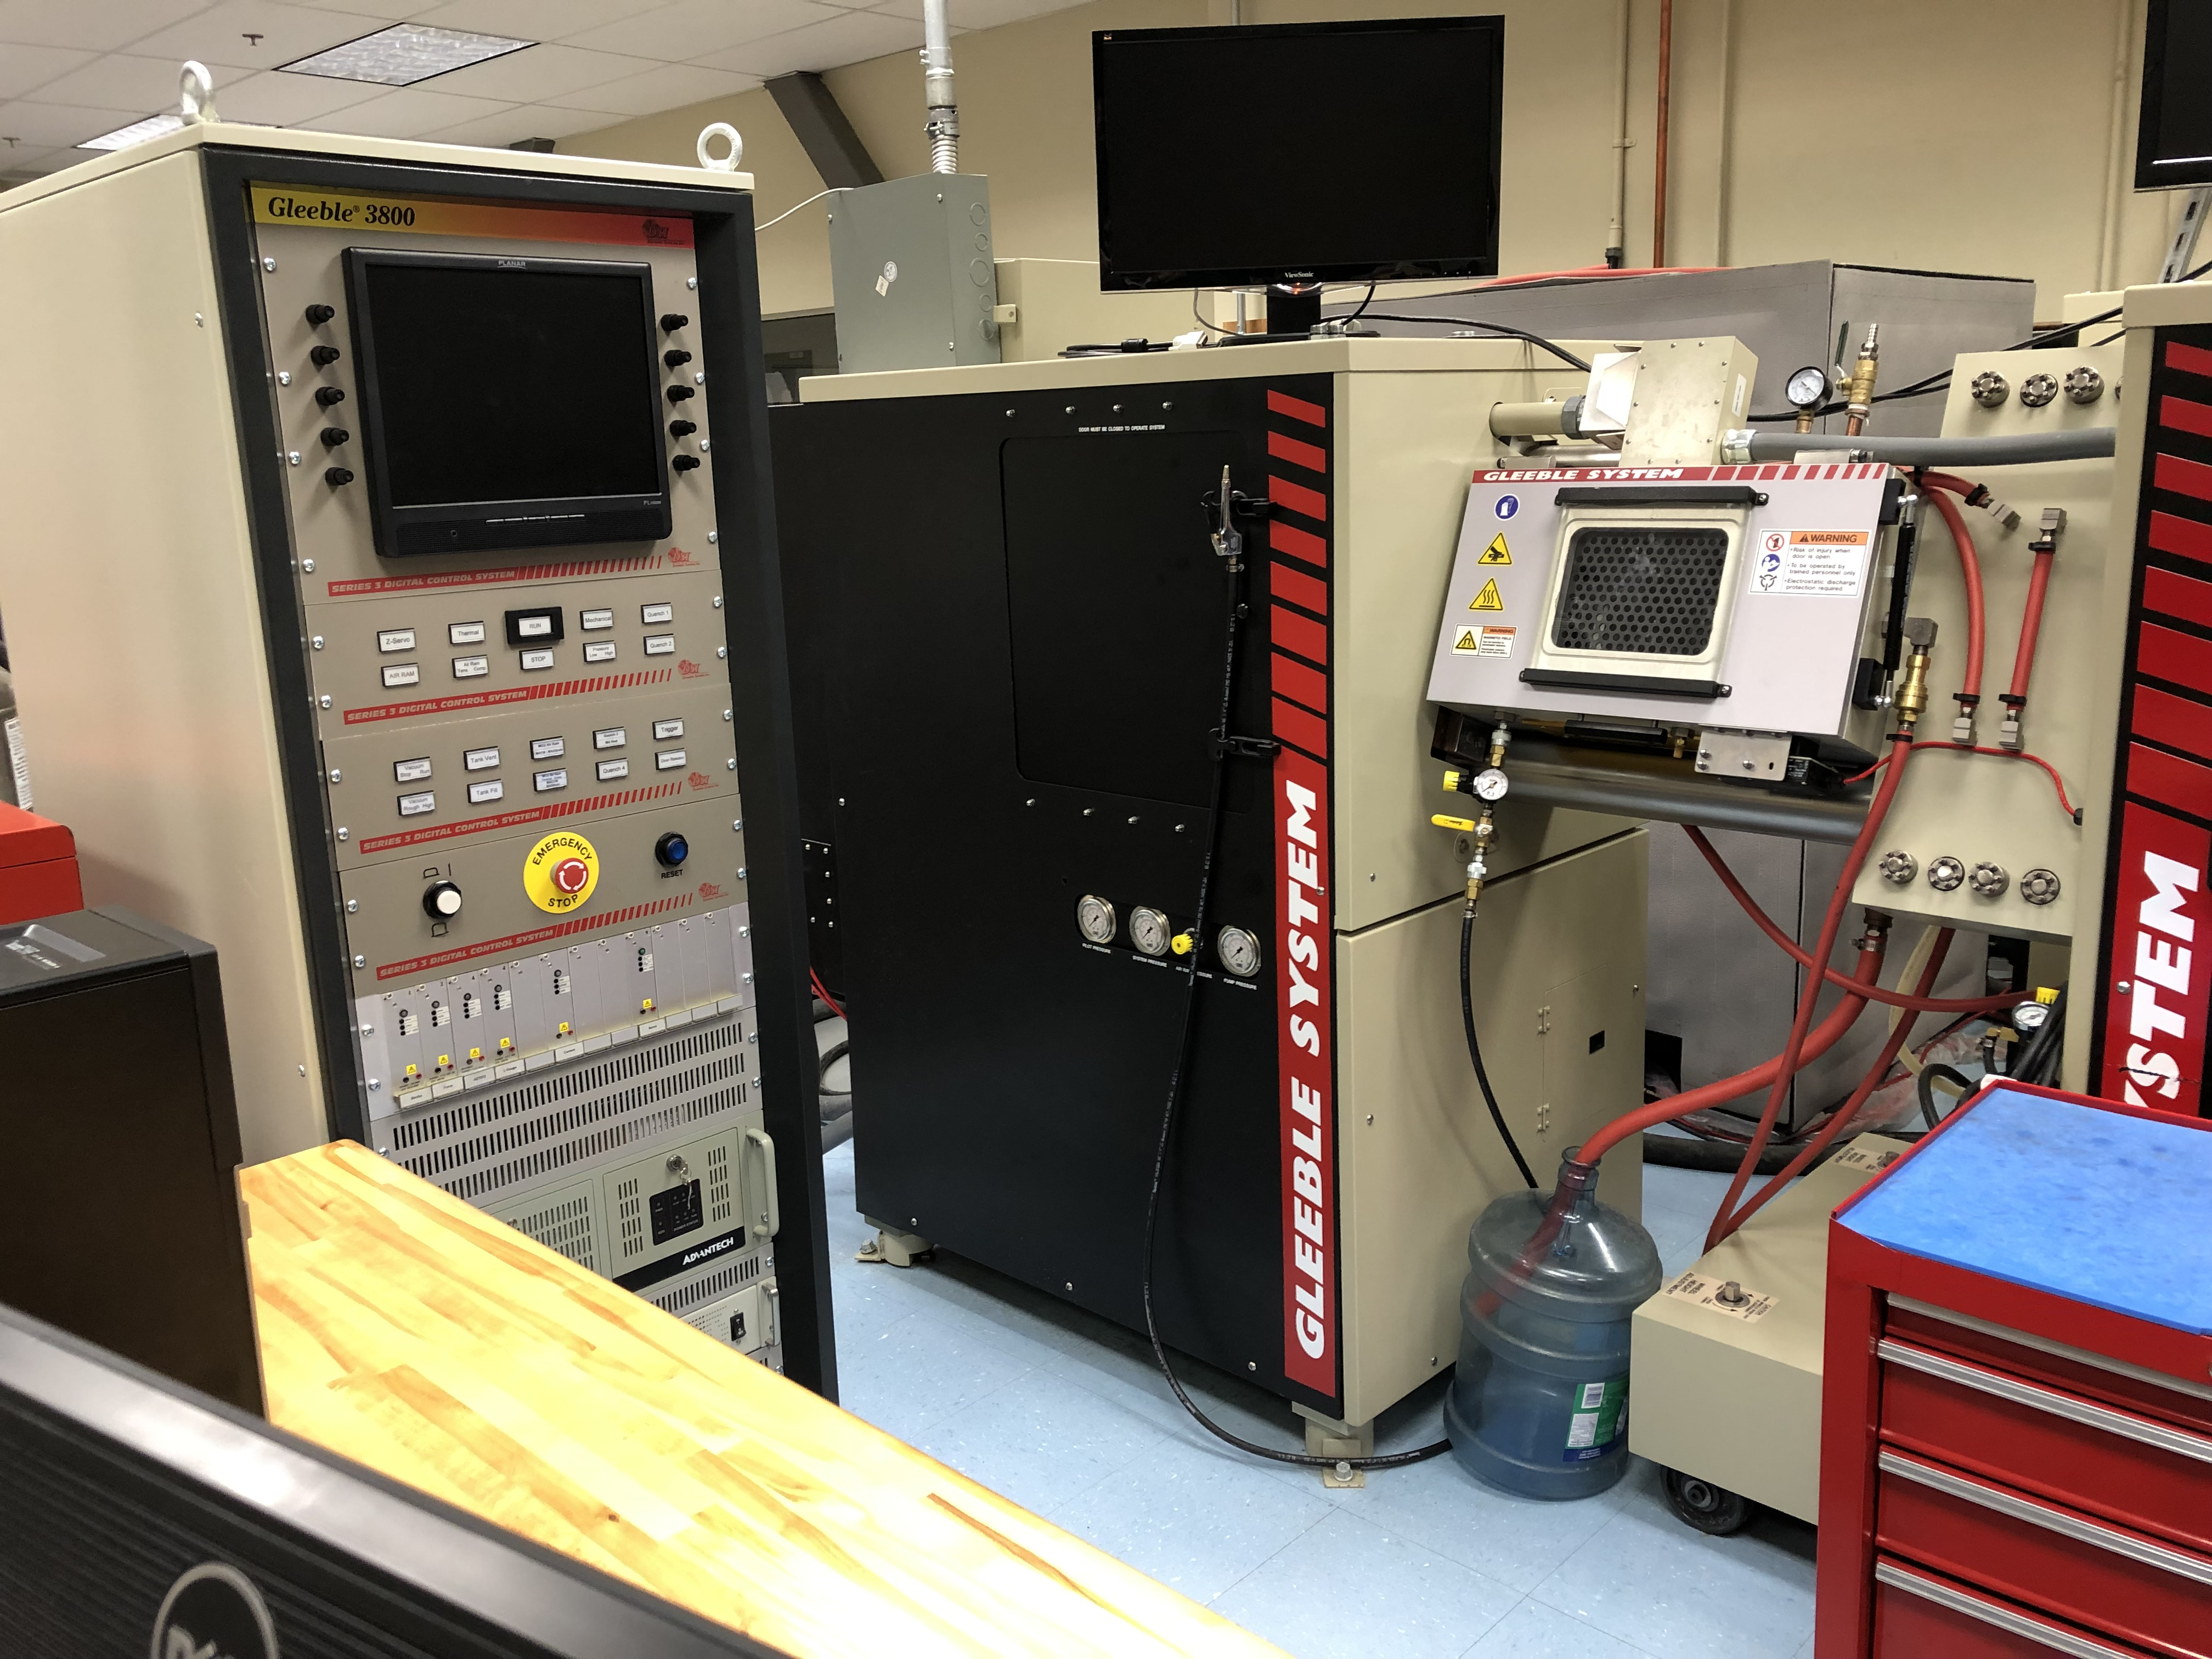
\includegraphics[width=0.7\columnwidth]{Figures/Gleeble-3800}
\caption{The Gleeble-3800 thermomechanical simulator system used for this study.}
\label{fig:Gleeble3800}
\end{figure}
Thin tantalum sheets were used as the lubricating material at the contact surface of the anvils and samples to minimize friction during testing.
Figure \ref{fig:Inside-Gleeble3800} shows the inside of the Gleeble thermomechanical simulator with the specimen in place. We used 3 thermocouples soldered to the specimen to record the temperature history during the test and to ensure that the specimen was at the correct temperature prior to testing.
\begin{figure}[H]

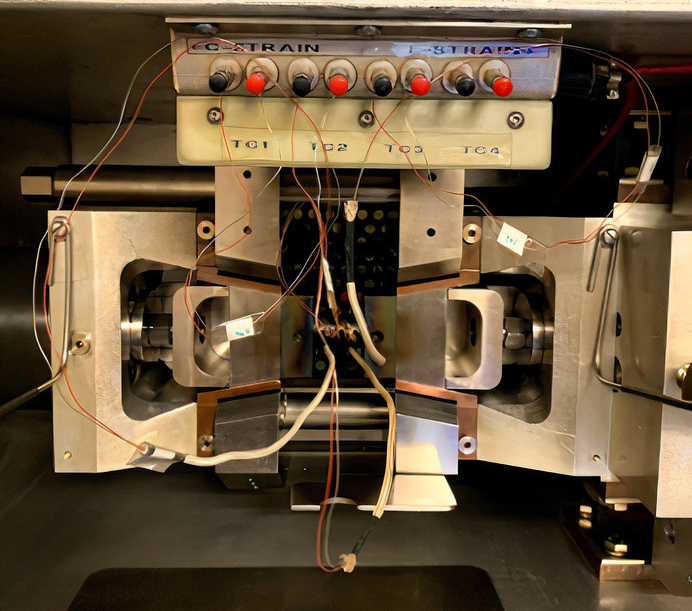
\includegraphics[width=0.7\columnwidth]{Figures/Gleeble-1}
\caption{The inside of the Gleeble-3800 thermomechanical simulator with the specimen in place.}
\label{fig:Inside-Gleeble3800}
\end{figure}

As shown in Figure \ref{fig:GleebleProcess}, the samples were heated to a temperature of $1260~\celsius$ with a heating rate of $2$~\celsius/s and held at this temperature for $5$~min to eliminate thermal gradients.
They were then cooled down with a rate of $1$~\celsius/s to the test temperature and then held at constant temperature for $1$~min before deformation.
During the compression phase, the temperature of the specimen is kept constant by the thermal control system of the machine.
After compression, the specimen is quickly quenched to freeze its microstructure for later analysis.
Figure \ref{fig:GleebleProcess} also shows the aspects of the specimens before and after the compression test: $h_0$ and $r_0$ are the height and radius before compression and $h$, $r_m$, and $r_t$ are the height, large radius, and small radius of the specimen after compression, respectively.
\begin{figure}[H]

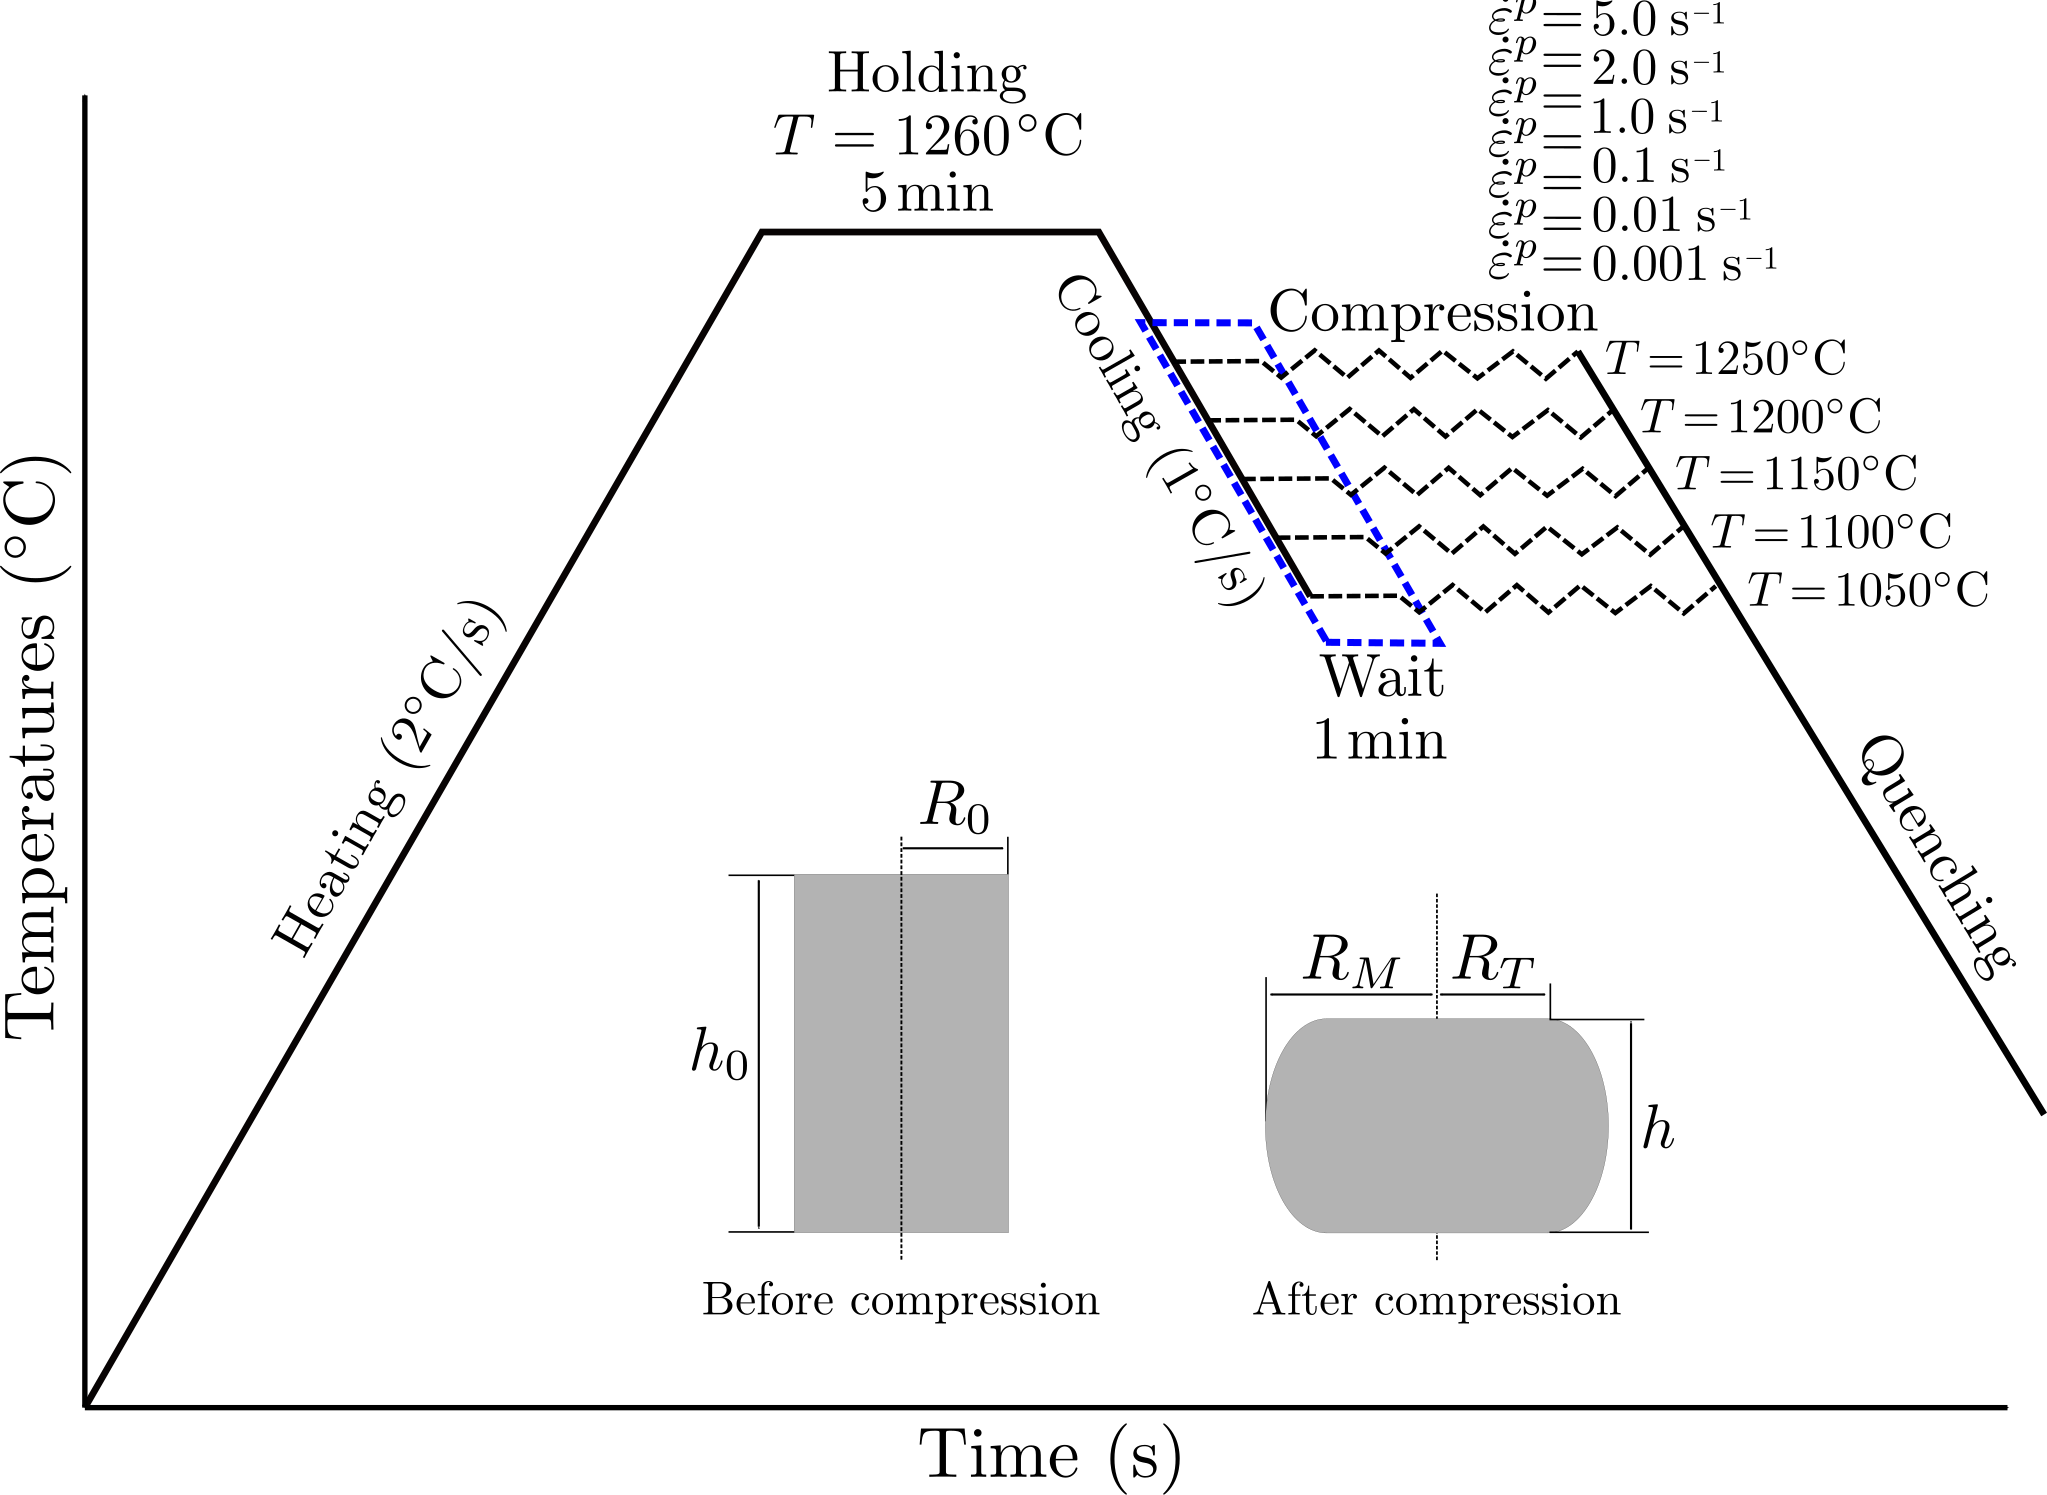
\includegraphics[width=0.8\columnwidth]{Figures/GleebleProcess}
\caption{\textls[-25]{Schematic diagram of the experimental process on the Gleeble-3800 thermomechanical simulator.}}
\label{fig:GleebleProcess}
\end{figure}

The stress--strain curves are automatically exported from the Gleeble thermomechanical simulator system as the true stress and true strain according to the L-gauge, where the formula to obtain the curves is given by $\sigma=F/A$ and $\varepsilon=\ln\left(1+\Delta h / h_0\right)$ or C-gauge, having the following formulas: $\sigma = 4F/\pi(d+\Delta d)^2$ and $\varepsilon = 2\ln\left(d/(d+\Delta d)\right)$ with $d = 2r_0$ and where $F$ is the force as measured by the Gleeble load cell.
As the raw data contain noises, the savgol\_filter method from the scipy library was used to remove noise and provide smoother data.
To allow further use of the data in numerical simulations, the elastic parts were removed.

%----------------------------------------------------------------------------------
\subsection{Compression Tests' Results\label{sec:ComTestResults}}
%----------------------------------------------------------------------------------

The set of flow stress $\sigma^y$ versus strain $\varepsilon$ curves obtained from compression tests performed on the Gleeble-3800 simulator for each test condition (6 strain rates and 5~temperatures) is presented in Figure \ref{fig:RawData}.
\begin{figure}[H]

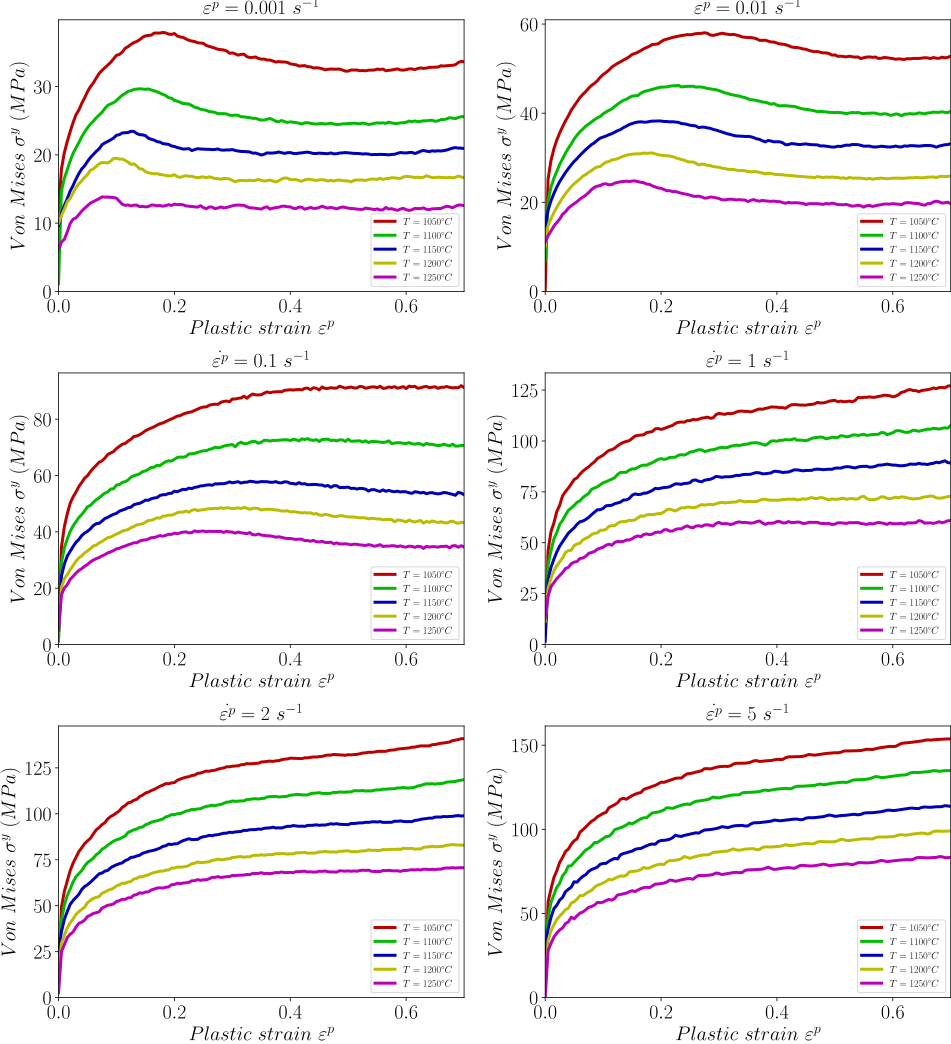
\includegraphics[width=0.99\columnwidth]{Figures/rawData}
\caption{Stress--strain curves of medium carbon alloy extracted from the Gleeble device at various temperatures $T$ and strain rates $\mdot\varepsilon$.}
\label{fig:RawData}
\end{figure}
All data curves contain $700$ equidistant strain values up to $\varepsilon=0.7$.
Therefore, there are $6$ strain rates and $5$ temperatures, and the database consists of 21,000 data points.
For the identification of the parameters of all the analytical models presented in this article, we restricted the database to 35 strain values between $0.02$ and $0.7$, with a step of $0.02$ (this is illustrated in Figure \ref{fig:RawData}, where the data used correspond to the dots on the graphs).
The overall behavior of these curves shows that the flow stress $\sigma^y$ increases with increasing strain rate $\mdot\varepsilon$, but decreases with increasing temperature $T$.
It should be noted that the strain also influences the flow stress.
Indeed, for the lowest strain rates $\mdot\varepsilon$, the flow stress $\sigma^y$ increases with the strain $\varepsilon$ until a value of about $\varepsilon=0.2$ to $0.3$ and then decreases to maintain a more or less constant value until the end of the test.
For the highest strain rates ($1~\ps$, $2~\ps$, and $5~\ps$), the flow stress increases throughout the test.
The slight increase in stress at low strain rates, when the strain is large, has been reported to be due to friction between the sample and the anvil during the test \cite{galos2022review}.
The frictional effect is also visible when testing at low strain rates, as the effect of lubrication decreases over time and friction, thus, increases.
The increase of stress observed at the beginning of the deformation and up to $0.1$ is due to work hardening (WH).
After $0.1$ and up to $0.2$, the flow stress shows a continuous reduction with increasing stress until a peak or an inflection of the work hardening rate.
This behavior indicates that thermal softening becomes more and more predominant until it exceeds WH.
At this step, the stress curve shows three different patterns with the increasing strain: (i) gradual decrease to a steady state with DRV/DRX softening.
This is the case for all deformation temperatures and strain rates between $0.001$ and $0.1~\ps$, except for those at $1050~\celsius$ and $1100~\celsius$; (ii) higher stress levels without significant softening and work hardening at $1050~\celsius$ and $1100~\celsius$ and a $0.1~\ps$ strain rate; (iii) a continuous increase with significant work hardening (all deformation temperatures and strain rate of $1~\ps$).
Therefore, it can be concluded that the softening due to DRX, characterized by a flow curve with a single peak followed by a steady-state flow, takes place at high temperatures and low strain rates.
In contrast, at higher strain rates and lower temperatures, the higher work hardening rate slows down the rate of softening due to DRX, and therefore, both the peak stress and the onset of steady-state flow are shifted to higher strain levels.
In fact, the drop observed in
stress is because of DRX occurrence at all temperatures and strain rates of $0.001$--$5~\ps$.

Figure \ref{fig:Micrography}a shows the microstructure obtained when the sample is held at $1260~\celsius$ for $5$~min and rapidly cooled to room temperature. From this image, large grains can be observed.
On the other hand, Figure \ref{fig:Micrography}b shows the microstructure after compression at $1150~\celsius$ with a $0.001~\ps$ strain rate.
To obtain this, the sample is heated up to $1260~\celsius$, then held for $5$ min and cooled down to $1150~\celsius$ to be held at this temperature for $1$ min before compression.
After compression, the sample is rapidly cooled to room temperature to preserve the microstructure.
From this image, full recrystallization can be observed and is in correlation with Figure \ref{fig:RawData}, where after the peak, a steady stress is observed that describes the end of the recrystallization.

%As an example, Figure \ref{fig:Micrography} shows the medium carbon microstructures held for $5$~min at $1260\celsius$ before and after the compression phase.
\begin{figure}[H]

\begin{subfigure}[b]{0.44\columnwidth}

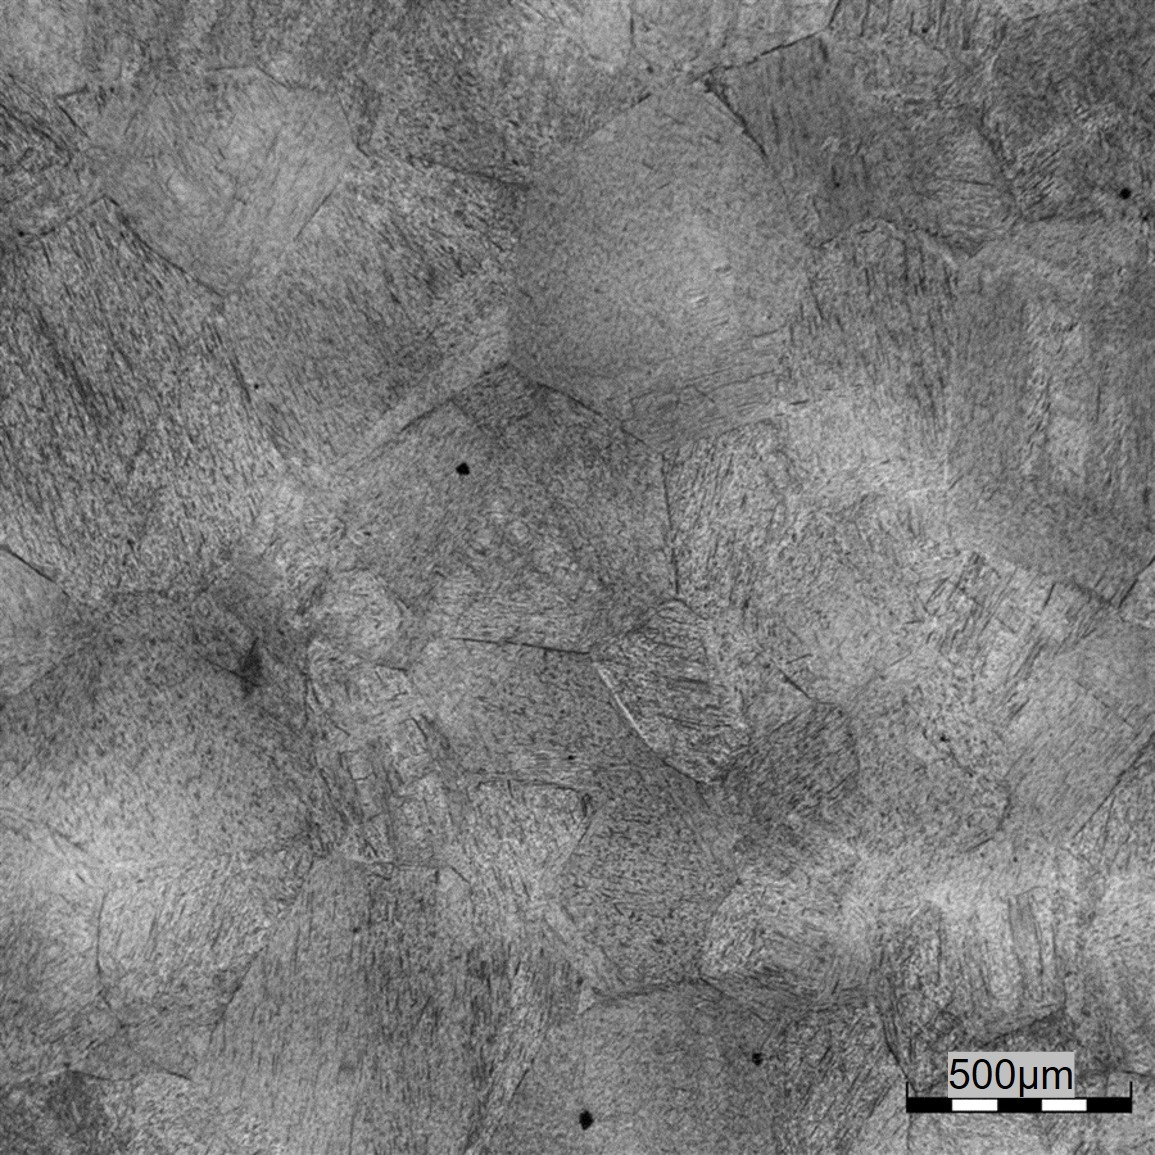
\includegraphics[width=\columnwidth]{Figures/BeforeCompM}
\caption{\centering Before hot compression}
\end{subfigure}
\hspace{10mm}
\begin{subfigure}[b]{0.44\columnwidth}

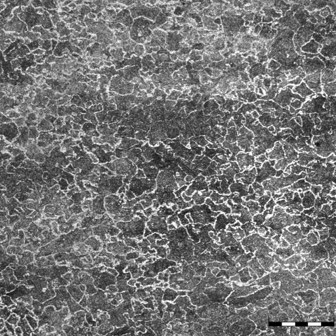
\includegraphics[width=\columnwidth]{Figures/AfterCompM}
\caption{\centering After hot compression}
\end{subfigure}
\vspace{6pt}
\caption{Optical micrographs of a medium carbon steel (\textbf{a}) before and (\textbf{b}) after hot compression at $1150~\celsius$ with a $0.001~\ps$ strain rate.}
\label{fig:Micrography}
\end{figure}
The material is in the single-phase austenite state at all of the test temperatures examined.
The data presented in Figure \ref{fig:RawData} will be utilized in the following section to determine the parameters of the $6$ flow laws proposed and to determine which model most closely aligns with the experimental results.

%----------------------------------------------------------------------------------
\section{Identification of Constitutive Flow Laws' Parameters\label{sec:ConstLaws}}
%----------------------------------------------------------------------------------
%----------------------------------------------------------------------------------
\subsection{The Johnson--Cook Model\label{sec:JC}}
%----------------------------------------------------------------------------------

The JC model, as mentioned above, is one of the most-widely used analytical models because it can be applied to many materials under different conditions of strain $\varepsilon$, strain rate $\mdot\varepsilon$, and temperature $T$.
However, the formulation of this model does not take into account the simultaneous effect of strain, strain rate, and temperature.
Indeed, it is formulated by describing the effect of each physical parameter ($\varepsilon$, $\mdot\varepsilon$, and $T$) separately as a factor in the mathematical expression of the model, hence its inability to describe the phenomenon of softening induced by temperature.
The equation that describes this model is given as follows \cite{Johnson-1983}:
\begin{equation}
\sigma^y=\left(A+B{\varepsilon^p}^{n}\right) \left[1+C\ln\left(\frac{\mdot\varepsilon}{\mdot\varepsilon_0}\right)\right] \left[1-\left(\frac{T-T_0}{T_m-T_0}\right)^{m}\right],\label{eq:Johnson--Cook}
\end{equation}
where $\sigma^y$ is the flow stress, $\varepsilon^p$ is the plastic strain, $A$ is the initial elastic limit of the material, $B$ is the strain hardening coefficient, $n$ is the strain hardening exponent, and $C$ and $m$ are the material constants that describe the strain rate hardening coefficient and the thermal softening coefficient, respectively.
The other values are reference values: $\mdot\varepsilon_0$ is the reference strain rate; $T_m$ and, thus, $T_0$ are the melting temperature ($1460~\celsius$ in our case) and the reference temperature, respectively.
For the determination of the parameters of the analytical models, the reference values for strain rate and temperature are $\mdot\varepsilon_0=0.001~\ps$ and $T_0=1050~\celsius$.
In our approach, the reference strain rate and reference temperature for identifying the JC model are the lowest values used during the test; however, sometimes, these values do not always give the best results for the model.

The procedure used to determine the parameters of the Johnson--Cook law is in accordance with the one proposed by Zeng \eal \cite{zeng2022constitutive}.
This method allows sequentially obtaining the $5$ parameters in the order $A$, $B$, $n$, $C$, and $m$.
Thus, according to the experimental data, the initial elastic limit of the material at the reference strain rate $\mdot\varepsilon_0$ and the reference temperature $T_0$ is $A=13.5143~\MPa$.
For the determination of the constants $B$ and $n$, from the results of the compression test at $T_0$ and $\mdot\varepsilon_0$, these two constants can then be determined by considering only the first term $\left(A+B{\varepsilon^p}^{n}\right)$ in Equation (\ref{eq:Johnson--Cook}).
Thus, here, $B=21.816~\MPa$ and $n=0.0746$.
Once the parameters $A$, $B$, and $n$ are known, the determination of $C$, considering only all the curves at $T=T_0$, then gives $C=0.3404$.
Finally, the last parameter $m$ is identified from the curves at $\mdot\varepsilon=\mdot\varepsilon_0$ and from knowledge of the parameters $A, B, C, n$ and gives $m=0.7057$.
All parameters of the Johnson--Cook model are reported in Table \ref{tab:JC}.

\begin{table}[H]

\caption{Parameter values of the Johnson--Cook flow law for a medium carbon steel.}
\newcolumntype{C}{>{\centering\arraybackslash}X}
\begin{tabularx}{\textwidth}{CCCCC}
\toprule
\boldmath{$A$~\bf (MPa)} & \boldmath{$B$~\bf (MPa)} & \boldmath{$n$} & \boldmath{$C$} & \boldmath{$m$} \\
\midrule
$13.5143$ & $21.816$ & $0.0746$ & $0.3404$ & $0.7057$ \\
\bottomrule
\end{tabularx}
\label{tab:JC}
\end{table}

The values predicted by the Johnson--Cook flow law (solid line) and the experimental values (dots) are compared in Figure \ref{fig:CompExp-JC-6}.
\begin{figure}[H]

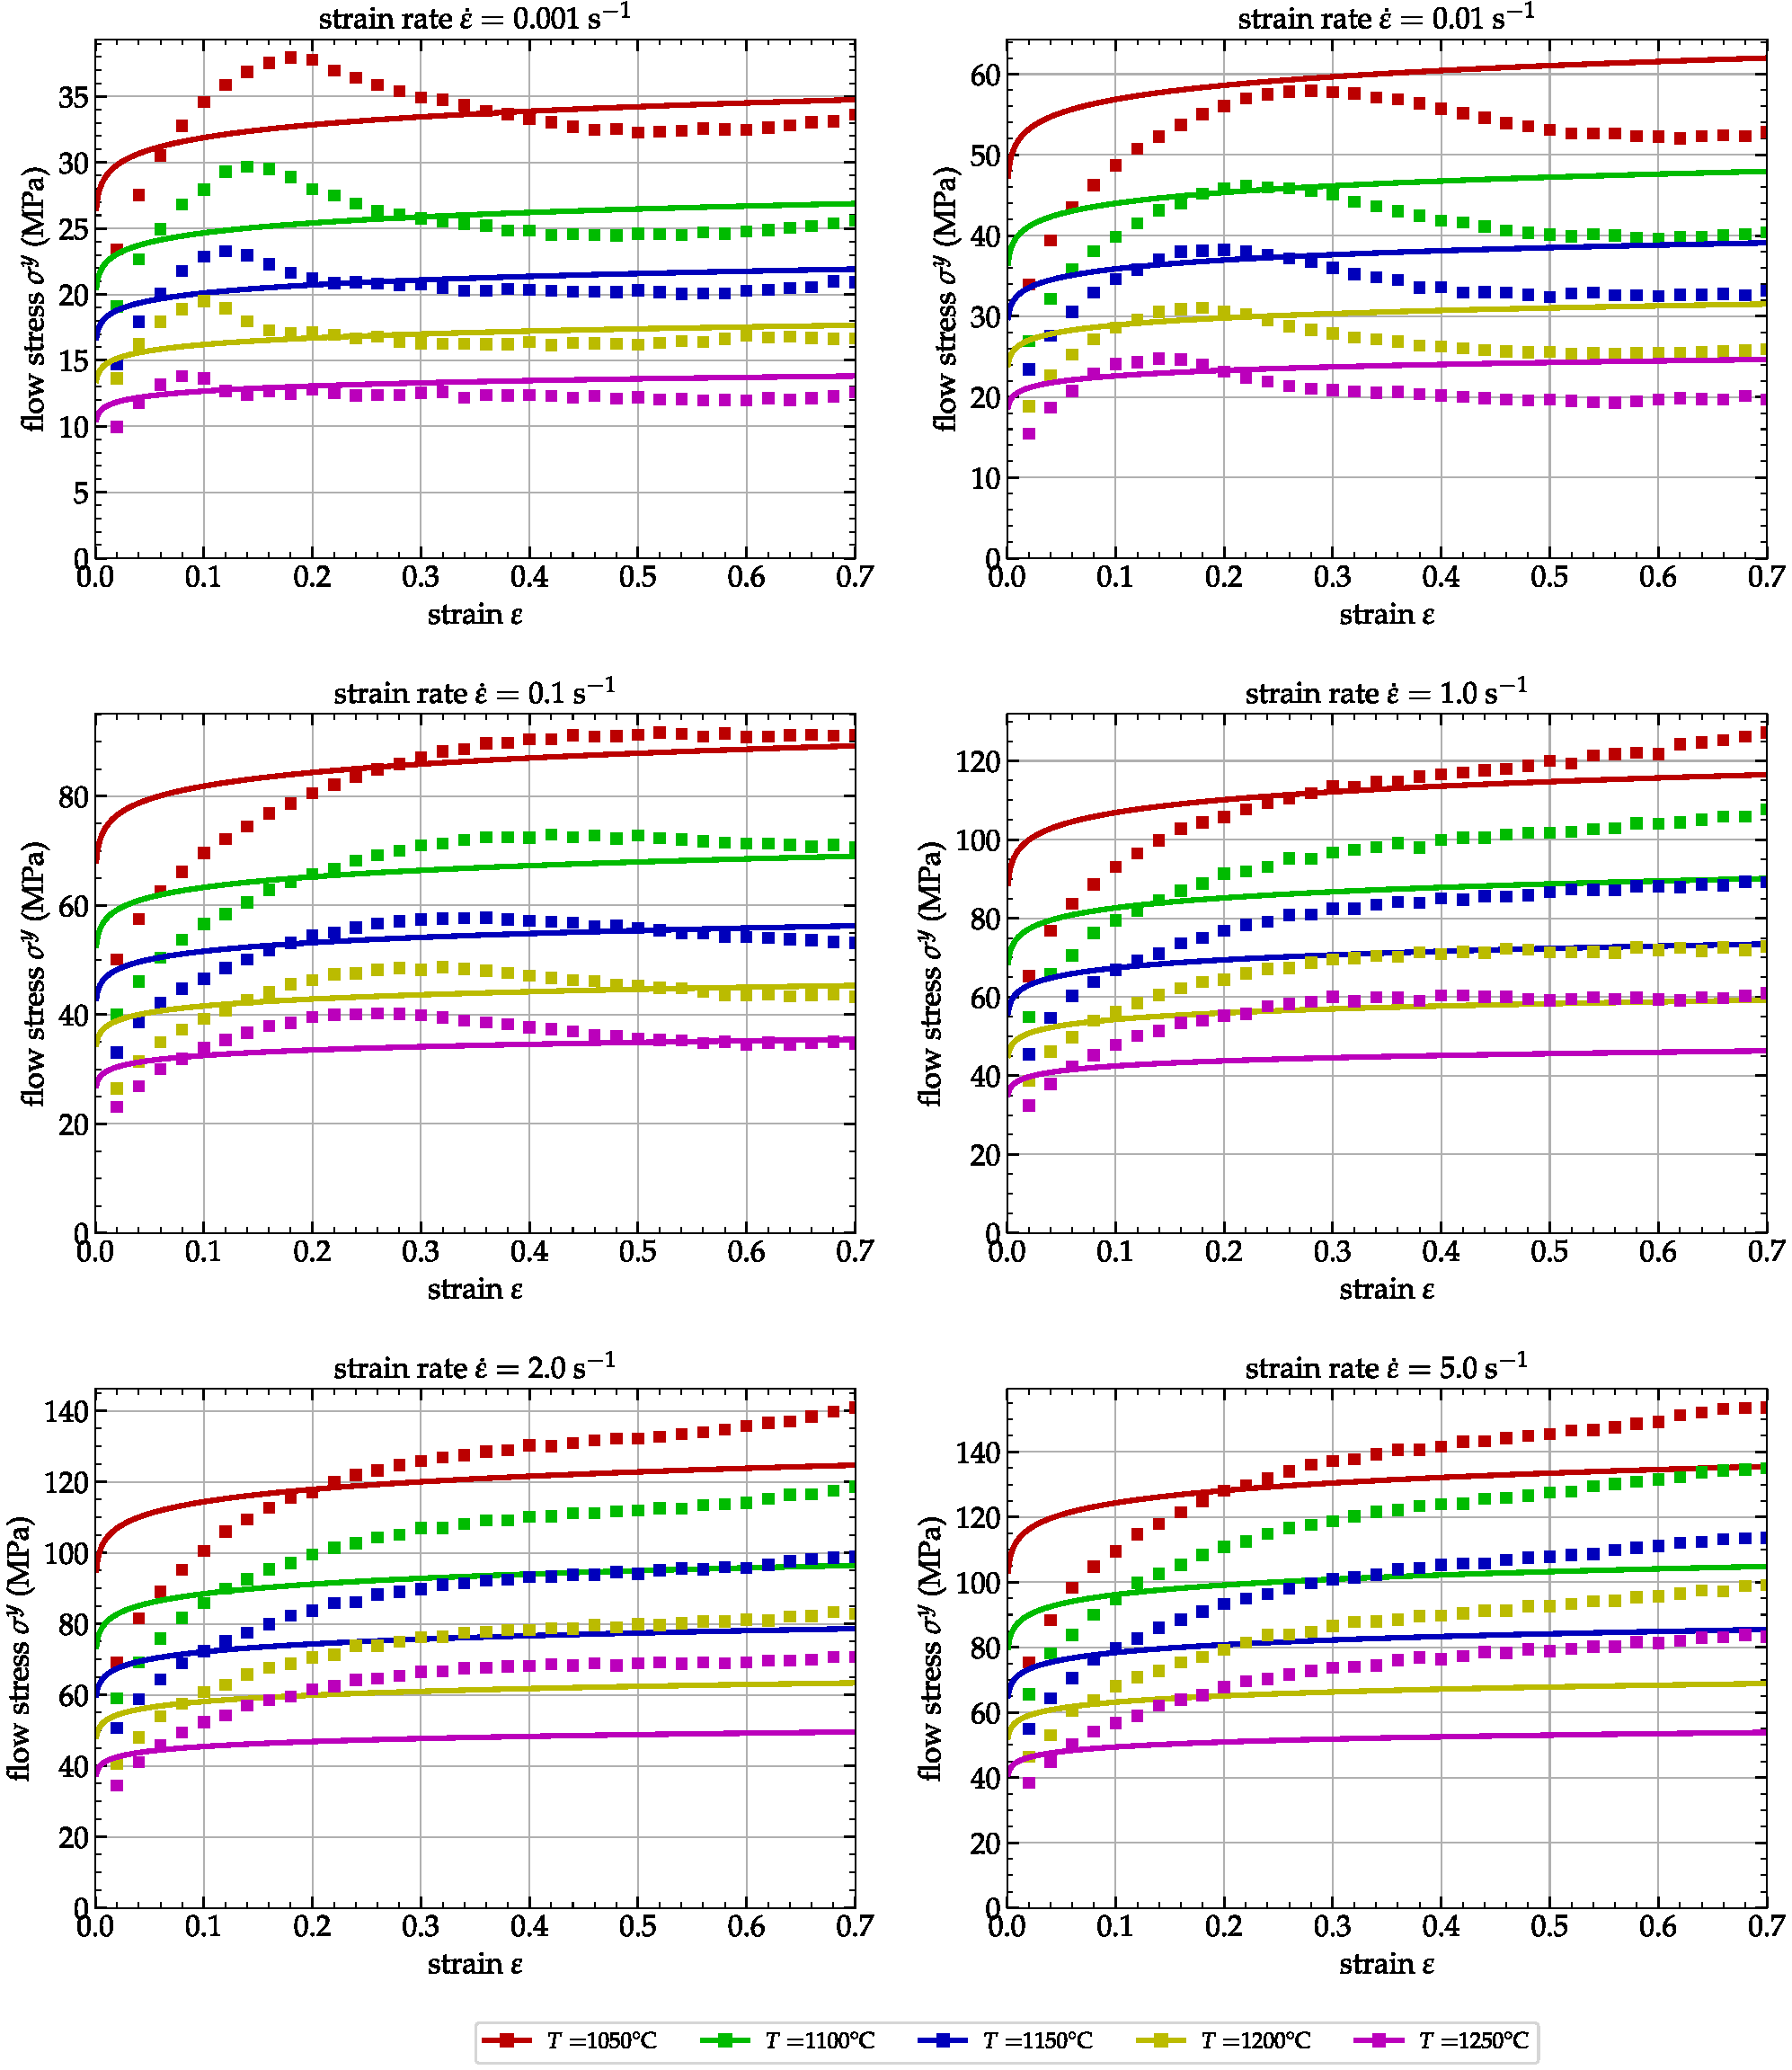
\includegraphics[width=0.99\columnwidth]{Figures/CompExp-JC-6}
\caption{{Comparison} %MDPI: Many figures are very similar. Please confirm there is no duplicate figure. No, every figure is different, the name of the figure correspond to the section, and everything is OK.
 between the experimental (dots) and predicted (lines) flow stresses $\sigma^y$ by the Johnson--Cook model.}
\label{fig:CompExp-JC-6}
\end{figure}
The JC model is unable to describe the evolution of the average flow stress for all strain and strain rate levels. The experimental flow stresses show a growth and then a decrease with strain, especially for low strain rates, while the JC model, by its formulation, only allows an increasing evolution of the flow stress $\sigma^y$ as a function of the strain independently of the strain rate value.
The discrepancy between the predicted and experimental values is large for low strains and sometimes acceptable for high strains.
As expected, the mathematical formulation of the Johnson--Cook flow law is unable to represent the stress drop at low strain rates, with the JC model increasing only monotonically with the strain.
Since most of the parameters are identified at low strain rates ($A$, $B$, and $n$), this results in a very poor fit of the model to the experimental data.

The accuracy and predictive ability of the models are usually assessed through certain coefficients such as the mean absolute relative error ($\MARE$) defined by Equation (\ref{eq:AARE}):
\begin{equation}
\MARE(\%) = \frac{1}{N} \sum_{i=1}^{N}{\left|\frac{\sigma_i^p -\sigma_i^e}{\sigma_i^e}\right|} \times 100, \label{eq:AARE}
\end{equation}
and the root-mean-squared error ($\RMSE$) defined by Equation (\ref{eq:RMSE}):
\begin{equation}
\RMSE (\MPa) = \sqrt{\frac{1}{N} \sum_{i=1}^{N} \left(\sigma_i^p - \sigma_i^e\right)^2}, \label{eq:RMSE}
\end{equation}
where $\sigma_i^e$ is the experimental value, $\sigma_i^p$ is the value predicted using the given model of the flow stress $\sigma^y$, and $N$ is the total number of data points used to compute those coefficients (in our case $N$ = 21,000).
For the JC model, $\MARE=14.05\%$ and $\RMSE=12.00~\MPa$.
As reported by Phaniraj \cite{Phaniraj-2003}, the correlation coefficient ($\R$) is not always an accurate measure to evaluate the reliability of the constitutive law especially in the case of a highly nonlinear functions because it only shows the correlation of the model with respect to the data and not its accuracy.
A good (high) value of $\R$ (close to $1$) does not necessarily mean a good prediction of the model, but simply establishes a good linearity correlation between the experiment and the prediction; we, therefore, avoided its use in our analysis.

%----------------------------------------------------------------------------------
\subsection{The Modified-Zerilli--Armstrong Model\label{sec:MZA}}
%----------------------------------------------------------------------------------

The MZA model, which is the modified form of the ZA model, like the JC model presented earlier, is one of the most-widely used models implemented in many FEA codes such as the Abaqus software.
The difference between the MZA model and JC model is related to the consideration of the three physical parameters to describe the reality observed from experiments.
In the JC model, the parameters are considered separately, while in the MZA model, they are considered simultaneously, and for that formulation, the MZA model is preferred over the JC model \cite{zhu2022thermal}.
However, the original form of the ZA model has some limitations due to the fact that it is considered as a two-term function (thermal and athermal functions), and to improve the formulation, Samantaray \eal \cite{Samantaray-2009} proposed a modified form given by the following equation:
\begin{equation}
\label{eq:MZA-model}
\sigma^y = \left(C_{1}+C_{2}{\varepsilon^p}^{n}\right) \exp\left[-\left(C_{3}+C_{4}\varepsilon^p\right)\left(T-T_0\right) + \left(C_{5}+C_{6}\left(T-T_0\right)\right)\ln\left( \frac{\mdot\varepsilon}{\mdot{\varepsilon}_0}\right)\right],
\end{equation}
where the $7$ coefficients $C_i$ and $n$ are the parameters of the model to be identified for a given material.
To obtain the parameters of the MZA model, we applied the method proposed by~\cite{Samantaray-2009}, and the parameters are summarized in Table \ref{tab:MZA}, while their predictions are plotted in \mbox{Figure \ref{fig:CompExp-MZA-6}}.
\begin{table}[H]

\caption{Parameter constants of the Modified-Zerilli--Armstrong model.}

\begin{adjustwidth}{-\extralength}{0cm}
%\centering %% If there is a figure in wide page, please release command \centering
\begin{minipage}{\fulllength}
\newcolumntype{C}{>{\centering\arraybackslash}X}
\begin{tabularx}{\textwidth}{CCCCCCC}
\toprule
\boldmath{$C_1$}~\bf (MPa) & \boldmath{$C_2$}~\bf (MPa) & \boldmath{$C_3$} & \boldmath{$C_4$} & \boldmath{$C_5$} & \boldmath{$C_6$} & \boldmath{$n$} \\
\midrule
$13.5143$ & $21.2591$ & $4.7902\times 10^{-3}$ & $1.4895\times 10^{-4}$ & $0.1389$ & $1.495\times 10^{-4}$ & $0.0621$ \\
\bottomrule
\end{tabularx}
\end{minipage}
\end{adjustwidth}
\label{tab:MZA}
\end{table}

It can be seen from this figure that both the MZA and JC models are not able to faithfully reproduce the experimental data, especially at low strain rates, but they are slightly better at higher strain rates.
The deviation between the predicted values and the experimental values is large because this model has a problem correctly describing the softening in its formulation.
For the MZA model, $\MARE=21.20\%$ and $\RMSE=19.57~\MPa$, showing an overall worse performance than the JC model, as reported in \cite{TizeMha-2022}.
In addition, it can be observed that, at high strain rates, the MZA model is not good either, even if there is no softening effect, and this can be explained by the fact that this model is formulated for quasi-static phenomena.


\begin{figure}[H]
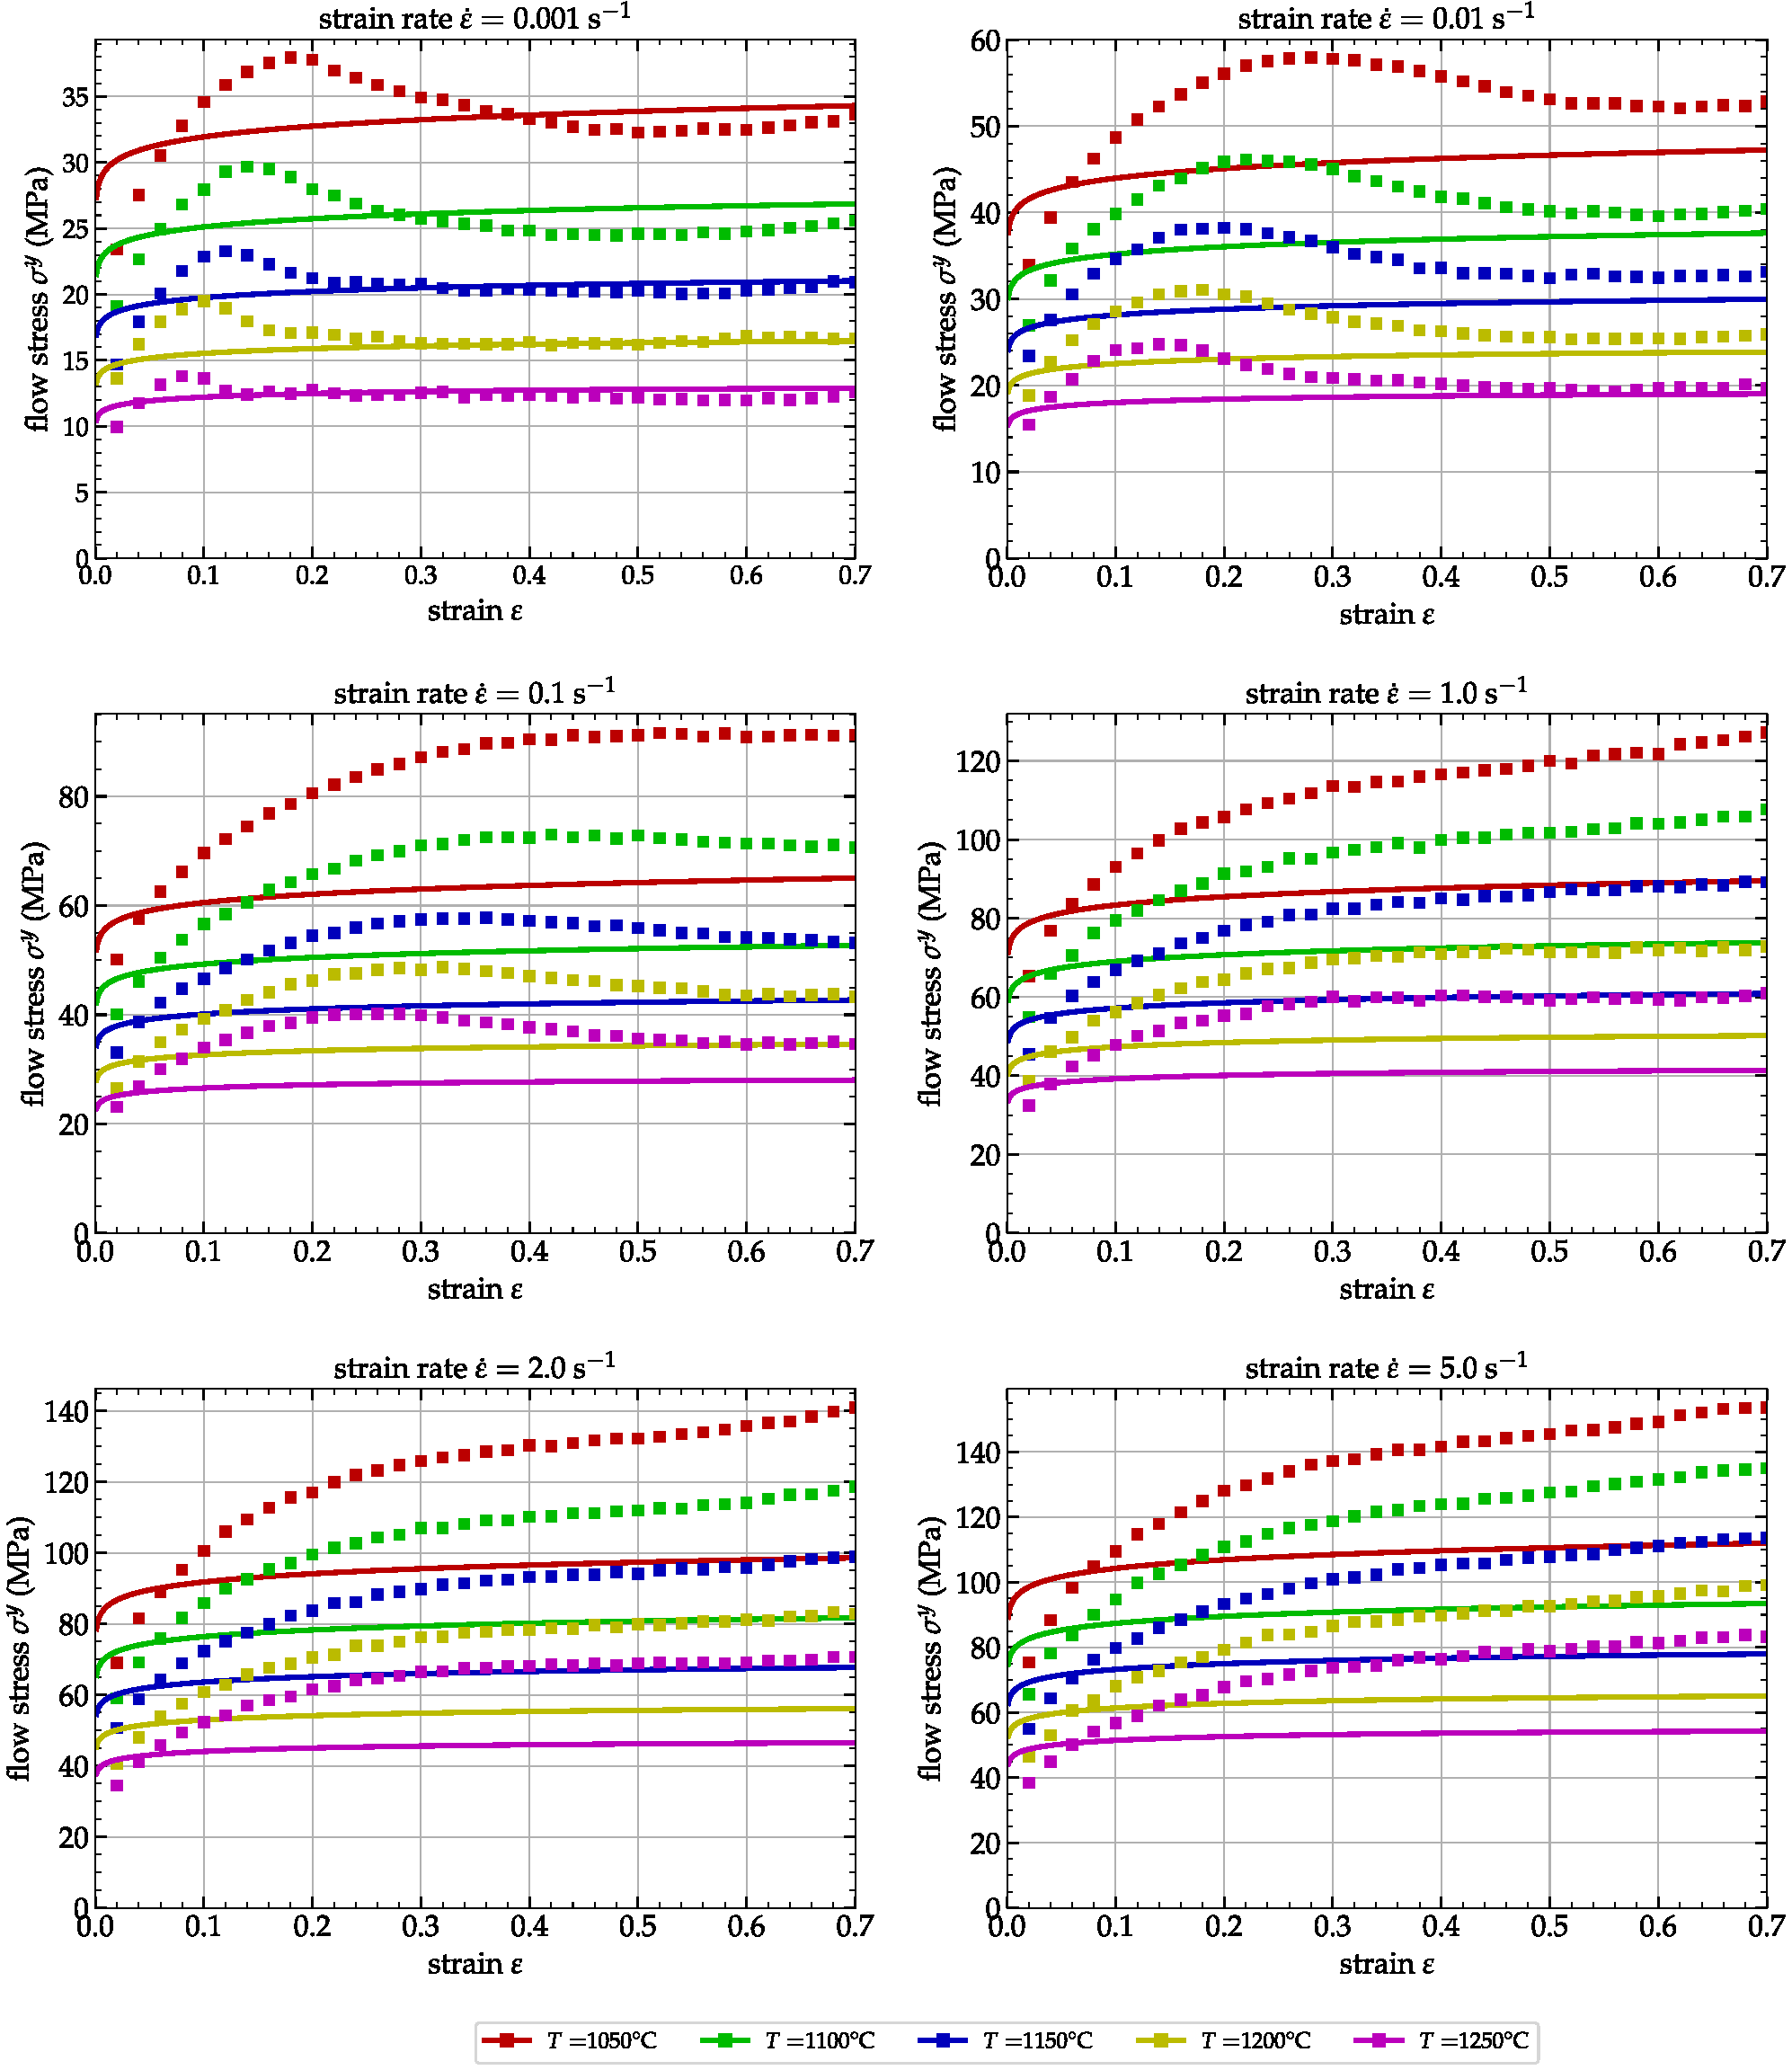
\includegraphics[width=0.93\columnwidth]
{Figures/CompExp-MZA-6}
\caption{Comparison between the experimental (dots) and predicted (lines) flow stresses $\sigma^y$ by the Modified-Zerilli--Armstrong model.}
\label{fig:CompExp-MZA-6}
\end{figure}


\vspace{-10pt}
%----------------------------------------------------------------------------------
\subsection{The Hansel--Spittel Model\label{sec:HSmodel}}
%----------------------------------------------------------------------------------

The Hansel--Spittel model \cite{Hensel-1978} is one of the least-known models in terms of integration in FEA codes, although its parameters can more easily be determined than those of the JC or MZA models.
Programming a simple identification script is sufficient to identify its parameters for a given material.
The equation of the HS model is given by the following~relation:
\begin{equation}
\sigma^y = A~\e{m_1T}~\varepsilon^{m_2}~\mdot\varepsilon^{m_3}~\e{({m_4}/{\varepsilon})}~(1+\varepsilon)^{m_5T}~\e{m_6\varepsilon}~\mdot\varepsilon^{m_7T}~T^{m_8}, \label{eq:HS}
\end{equation}
where again, $\sigma^y$ is the flow stress, $\varepsilon$ is the strain, $\mdot\varepsilon$ is the strain rate, and $T$ is the temperature, as proposed earlier.
The coefficients $A$ and $m_i$ are the 9 parameters of the model to be identified.
However, this model has some shortcomings, notably related to the fact that its accuracy varies according to the number of parameters taken into account during the identification.
For its identification, several authors restrict its expression to a reduced number of only $5$ or $6$ $m_i$ parameters, by forcing a zero value for the other \mbox{parameters \cite{chadha2018approach, Mehtedi-2015, rudnytskyj2020constitutive}.}

In the present study, the best results were obtained by taking the model defined by only the first 7 $m_i$ terms of the Equation (\ref{eq:HS}), so that $m_8=0$.
From the experimental data obtained during the compression tests, an identification procedure based on the use of the LMFIT optimizer \cite{Newville-2016} allowed computing the parameters reported in Table
 \ref{tab:HS}.

\begin{table}[H]

\caption{Parameter values of the Hansel--Spittel flow law for the medium carbon steel.}
\newcolumntype{C}{>{\centering\arraybackslash}X}
\begin{tabularx}{\textwidth}{CCCCC}
\toprule
\boldmath{$A$} & \boldmath{$m_1$} & \boldmath{$m_2$} & \boldmath{$m_3$} & \boldmath{$m_4$} \\
\midrule
$5.954\times 10^{3}$ & $-3.3576\times10^{-3}$ & $0.2641$ & $-0.0868$ & $2.2688\times10^{-4}$ \\
\toprule
& \boldmath{$m_5$} & \boldmath{$m_6$} & \boldmath{$m_7$} & \boldmath{$m_8$} \\ %MDPI: Please confirm if all the bold should be kept: You can remove the bold, if it does not correspond to the editorial line of the journal.
\midrule
& $-4.2163\times10^{-4}$ & $-0.0561$ & $2.264\times10^{-4}$ & $0$ \\
\bottomrule
\end{tabularx}
\label{tab:HS}
\end{table}

A comparison of the values predicted by the HS model and the experimental values is presented in Figure \ref{fig:CompExp-HS-6}, where the dots represent the experimental values and the solid lines are the values predicted by the Hansel--Spittel flow law.
For the HS model, \mbox{$\MARE=7.75\%$} and $\RMSE=3.80~\MPa$.
It appears that both this model and the previous ones do not adequately predict the experimental one, and the difference is relatively significant for all strain rates below $1~\ps$.
This shows that this model is not appropriate for the characterization of this alloy, particularly because of the strong nonlinear behavior observed for low strain rate values.
The DRX phenomenon cannot be reproduced by this type of~model.

\begin{figure}[H]

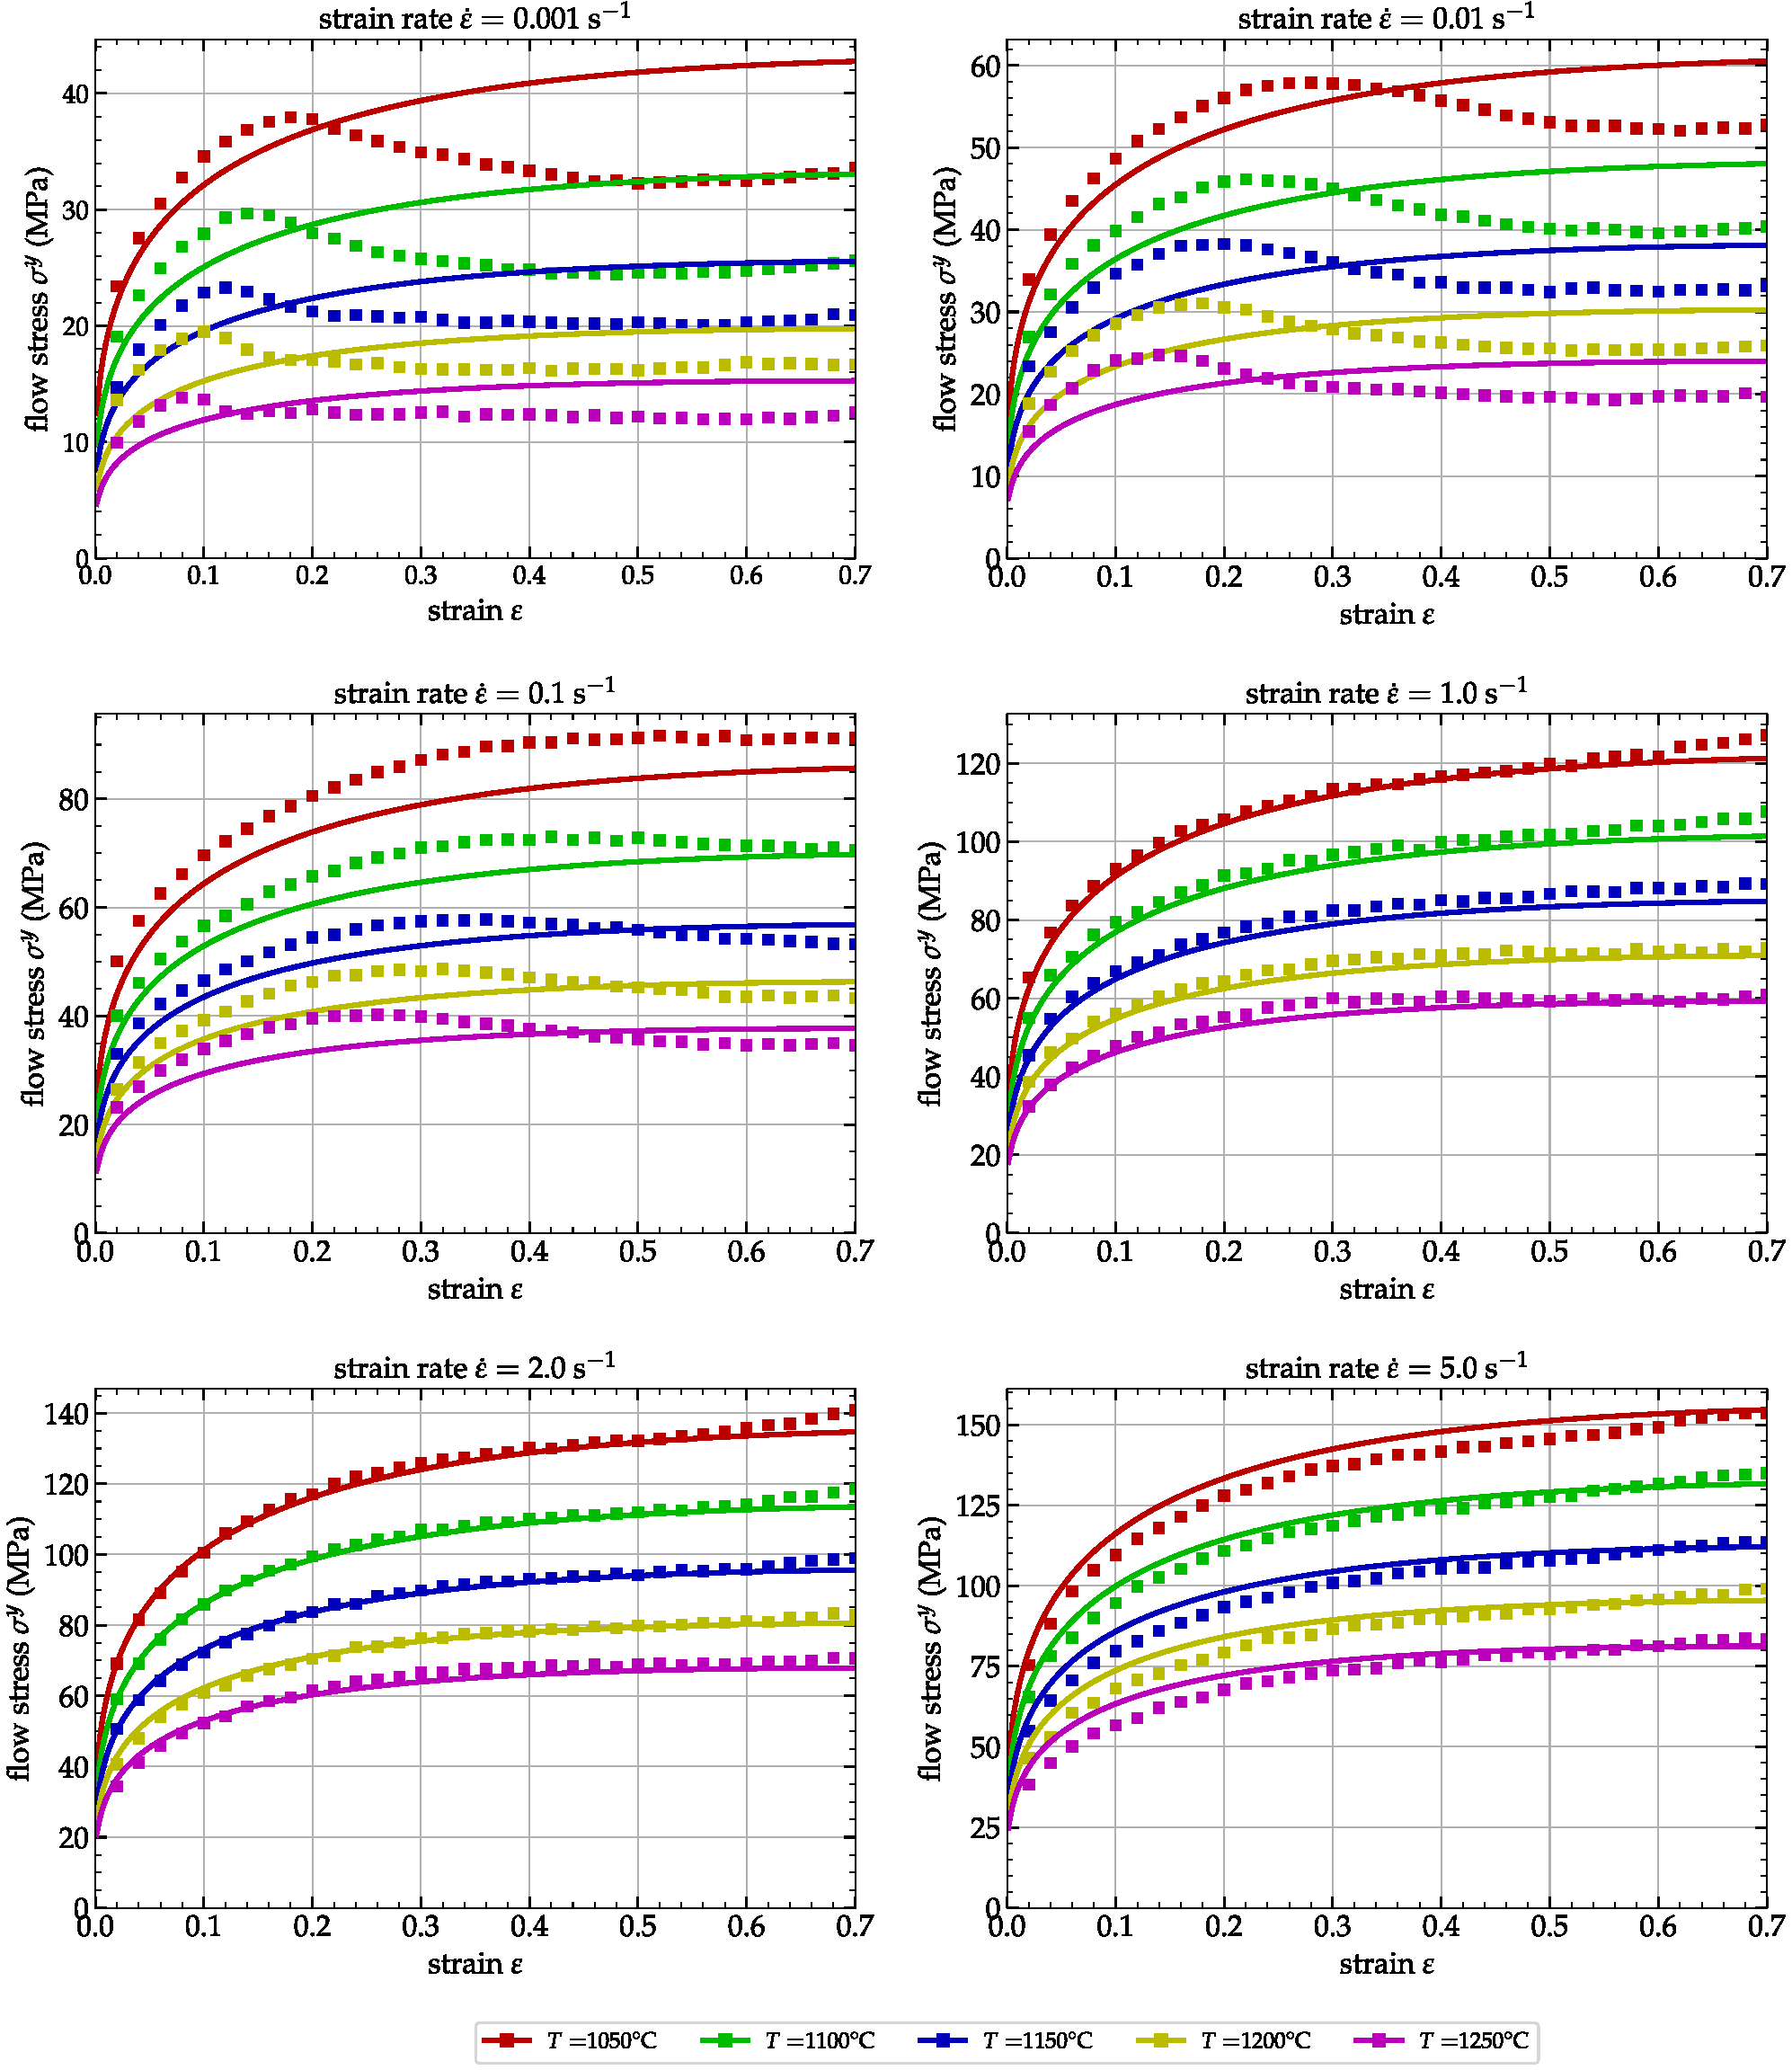
\includegraphics[width=0.9\columnwidth]
{Figures/CompExp-HS-6}
\caption{Comparison between the experimental (dots) and predicted (lines) flow stresses $\sigma^y$ by the Hansel--Spittel model.}
\label{fig:CompExp-HS-6}
\end{figure}

%----------------------------------------------------------------------------------
\subsection{The Arrhenius Model\label{sec:ARmodel}}
%----------------------------------------------------------------------------------

The Arrhenius type model \cite{Sellars-1966} is one of the most-used models in the framework of material forming, especially when it comes to studying the material microstructure.
The model takes into account the physical phenomena describing the behavior of the material in the formulation of the relationships between the stress $\sigma^y$, the strain $\varepsilon$, the strain rate $\mdot\varepsilon$, and the temperature $T$ expressed as the power law, exponential law, and hyperbolic sine.
This makes it easier to describe the softening phenomenon observed in the material due to increasing temperature.
The following equations describe the Arrhenius model:
\begin{equation}
\mdot\varepsilon =
\begin{cases}
A_1 \sigma^{y^{n_1}} \exp{\left(-\frac{Q}{RT}\right)} & \alpha\sigma^y < 0.8\\
A_2 \exp(\beta\sigma^y) \exp{\left(-\frac{Q}{RT}\right)} & \alpha\sigma^y > 1.2\\
A_3 \left[\sinh{\left(\alpha\sigma^y\right)}\right]^{n_2} \exp{\left(-\frac{Q}{RT}\right)} & \text{for all }\sigma^y
\end{cases}
\label{eq:ArDef}
\end{equation}
with:
\begin{equation}
Z = \mdot\varepsilon \exp{\left(\frac{Q}{RT}\right)}, \label{eq:ArZ}
\end{equation}
where $Z$ is the Zenner--Hollomon parameter \cite{Zener-1944}, $\mdot\varepsilon$ is the strain rate ($\ps$), $Q$ is the apparent activation energy ($\text{J~mol}^{-1}$), $R$ is the universal gas constant ($8.314~\text{J~mol}^{-1} \text{K}^{-1}$), $T$ is the absolute temperature (K), $\sigma^y$ is the flow stress (MPa) for a given strain, strain rate, and temperature, and $A_1$, $A_2$, $A_3$, $n_1$, $n_2$, $\alpha$, and $\beta=\alpha~n_1$ are dependent on the material.
The corresponding values are independent of the temperature and are obtained from the stress--strain curves at different strain rates and temperatures by the regression method.
Combining Equations (\ref{eq:ArDef}) and (\ref{eq:ArZ}) allows expressing the flow stress $\sigma^y$ as a function of the $Z$~parameter:
\begin{equation}
\sigma^y = \frac{1}{\alpha} \ln\left\{\left(\frac{Z}{A}\right)^{1/n} + \left[1 + \left(\frac{Z}{A}\right)^{2/n}\right]^{1/2}\right\}
\end{equation}

To obtain the constitutive equation, all the parameters $A$, $Q$, $\alpha$, and $n$ must be determined for a given material.
The strain has a significant nonlinear influence on the behavior of the material by the strain hardening and softening mechanisms at high values of deformation.
A strain-dependent factor must, therefore, be taken into account in the Arrhenius model, which leads to the definition of the modified Arrhenius model for which the $A$, $Q$, $\alpha$, and $n$ parameters are expressed as a function of the strain $\varepsilon$ by means of polynomial functions of degree $m$ (varying from $1$ to $9$) of the form:
\begin{equation}
A(\varepsilon) = \exp{\left[\ln\!A_0 + \ln\!A_1\varepsilon + \ln\!A_2\varepsilon^2 + \ln\!A_3\varepsilon^3 + \cdots + \ln\!A_m\varepsilon^m\right]}
\label{eq:ArA}
\end{equation}
\begin{equation}
Q(\varepsilon) = Q_0 + Q_1\varepsilon + Q_2\varepsilon^2 + Q_3\varepsilon^3 + \cdots + Q_m\varepsilon^m
\label{eq:ArQ}
\end{equation}
\begin{equation}
\alpha(\varepsilon) = \alpha_0 + \alpha_1\varepsilon + \alpha_2\varepsilon^2 + \alpha_3\varepsilon^3 + \cdots + \alpha_m\varepsilon^m
\label{eq:Aralpha}
\end{equation}
\begin{equation}
n(\varepsilon) = n_0 + n_1\varepsilon + n_2\varepsilon^2 + n_3\varepsilon^3 + \cdots + n_m\varepsilon^m
\label{eq:Arn}
\end{equation}

The determination of the order $m$ of the polynomials defining Equations (\ref{eq:ArA})--(\ref{eq:Arn}) depends on the ability of the model to represent the nonlinear dependence of the stress on strain and its generalization.
The values $\ln\!A_i$, $\alpha_i$, $n_i$, and $Q_i$ ($i=0,1,2,3,\cdots,m$) are the coefficients of the polynomials used to determine using a regression method.
Setting $m=9$ gives the best results, and the corresponding parameters are reported in Table \ref{tab:AR}.
\begin{table}[H]
\centering
\caption{Parameter values of the Arrhenius flow law for the medium carbon steel.}
\newcolumntype{L}{>{\raggedright\arraybackslash}X}
\begin{tabularx}{\textwidth}{LLLL}
\toprule
\multicolumn{1}{c}{\boldmath{$\alpha_i$}} & \multicolumn{1}{c}{\boldmath{$Q_i~(\times 10^{-6})$}} & \multicolumn{1}{c}{\boldmath{$\ln\!A_i$}} & \multicolumn{1}{c}{\boldmath{$n_i$}} \\
\midrule
$\alpha_0=0.0407$ & $Q_0=0.467$ & $\ln\!A_0=35.8092$ & $n_0=4.8217$ \\
$\alpha_1=-0.5167$ & $Q_1=-0.6517$ & $\ln\!A_1=-58.822$ & $n_1=3.2814$ \\
$\alpha_2=6.3912$ & $Q_2=7.6084$ & $\ln\!A_2=740.3303$ & $n_2=71.5963$ \\
$\alpha_3=-47.3364$ & $Q_3=-48.016$ & $\ln\!A_3=-5.0493\times 10^{3}$ & $n_3=-1.9562\times 10^{3}$ \\
$\alpha_4=220.0014$ & $Q_4=66.795$ & $\ln\!A_4=1.1305\times 10^{4}$ & $n_4=1.4461\times 10^{4}$ \\
$\alpha_5=-654.4553$ & $Q_5=468.8898$ & $\ln\!A_5=2.022\times 10^{4}$ & $n_5=-5.431\times 10^{4}$ \\
$\alpha_6=1.2421\times 10^{3}$ & $Q_6=-2.3032\times 10^{3}$ & $\ln\!A_6=-1.5387\times 10^{5}$ & $n_6=1.1761\times 10^{5}$ \\
$\alpha_7=-1.4523\times 10^{3}$ & $Q_7=4.3707\times 10^{3}$ & $\ln\!A_7=3.1798\times 10^{5}$ & $n_7=-1.4882\times 10^{5}$ \\
$\alpha_8=952.0619$ & $Q_8=-3.9394\times 10^{3}$ & $\ln\!A_8=-2.9725\times 10^{5}$ & $n_8=1.0239\times 10^{5}$ \\
$\alpha_9=-267.4994$ & $Q_9=1.397\times 10^{3}$ & $\ln\!A_9=1.0759\times 10^{5}$ & $n_9=-2.9621\times 10^{4}$ \\
\bottomrule
\end{tabularx}
\label{tab:AR}
\end{table}
This modified form of the Arrhenius behavior law allows an accurate and reliable prediction over a wide range of temperatures and strain rates.
Equation (\ref{eq:ArStress}) is finally used to compute the flow stress $\sigma^y$ from the strain $\varepsilon$, the strain rate $\mdot\varepsilon$, and the temperature $T$:
\begin{equation}
\sigma^y = \frac{1}{\alpha(\varepsilon)} \ln\left\{\left(\frac{\mdot\varepsilon \exp{\left(\frac{Q(\varepsilon)}{RT}\right)}}{A(\varepsilon)}\right)^{\frac{1}{n(\varepsilon)}} + \left[1 + \left(\frac{\mdot\varepsilon \exp{\left(\frac{Q(\varepsilon)}{RT}\right)}}{A(\varepsilon)}\right)^{\frac{2}{n(\varepsilon)}}\right]^{\frac{1}{2}}\right\}
\label{eq:ArStress}
\end{equation}

Figure \ref{fig:CompExp-AR-6} shows a comparison of the values predicted by the Arrhenius model and the experimental values.
The difference between the experimental and predicted values is small.
However, for the strain rate $\mdot\varepsilon = 0.01~\ps$ and for the two low temperature values, the AR model is unable to predict the softening.
For the AR model, $\MARE=3.56\%$ and $\RMSE=2.18~\MPa$.


%----------------------------------------------------------------------------------
\subsection{The PTM Model\label{sec:PTM}}
%----------------------------------------------------------------------------------

The PTM model \cite{TizeMha-2022} is a generalized formulation of the MZA model presented in Section \ref{sec:MZA}.
When establishing its formulation, the main shortcomings of the MZA model were taken into account, in order to render the PTM model flexible for any type of material studied because it removes the need for a limited number of parameters as in the MZA model.
Its construction is based on the use of polynomial functions, as is the case in the AR model.
Thus, the physical parameters' dependent intrinsic functions of the PTM model allow adjusting the model according to the degree selected for each of the 4 constituent polynomials, which provides a good fit for each function.
The equation describing the PTM model is, therefore, given by:

\begin{adjustwidth}{-\extralength}{0cm}
%\centering %% If there is a figure in wide page, please release command \centering
\begin{equation}
\label{eq:PTM-model}
\sigma^y = \left(\sum_{i=0}^{q}{A_i{\varepsilon^p}^{i}}\right) \exp\left[\left(\sum_{j=0}^{r}{B_j{\varepsilon^p}^{j}}\right)\left(T-T_0\right) + \left(\sum_{k=0}^{s}\left(\sum_{l=0}^{t}{C_k^l{\varepsilon^p}^{l}} \right)\left(T-T_0\right)^k \right)\ln\left( \frac{\mdot\varepsilon}{\mdot{\varepsilon}_0}\right)\right]
\end{equation}
\end{adjustwidth}
\vspace{6pt}
where $A_i, B_j, C_k^l$ are the parameters (Table \ref{tab:PTM}) of the model to be identified using the procedure proposed in \cite{TizeMha-2022}.
Quantities $q$, $r$, $s$, and $t$ define the degree of the polynomials used to describe the behavior of the material.
The larger these quantities, the greater the number of parameters that need to be identified for the PTM model.
The determination of the parameters of this model was performed thanks to the LMFIT Python library \cite{Newville-2016} (for more details about this model, we refer the reader to our previous work \cite{TizeMha-2022}).
Thus, all the parameters of this model were calculated with $q=5$, $r=5$, $s=1$, and $t=5$.


\begin{figure}[H]

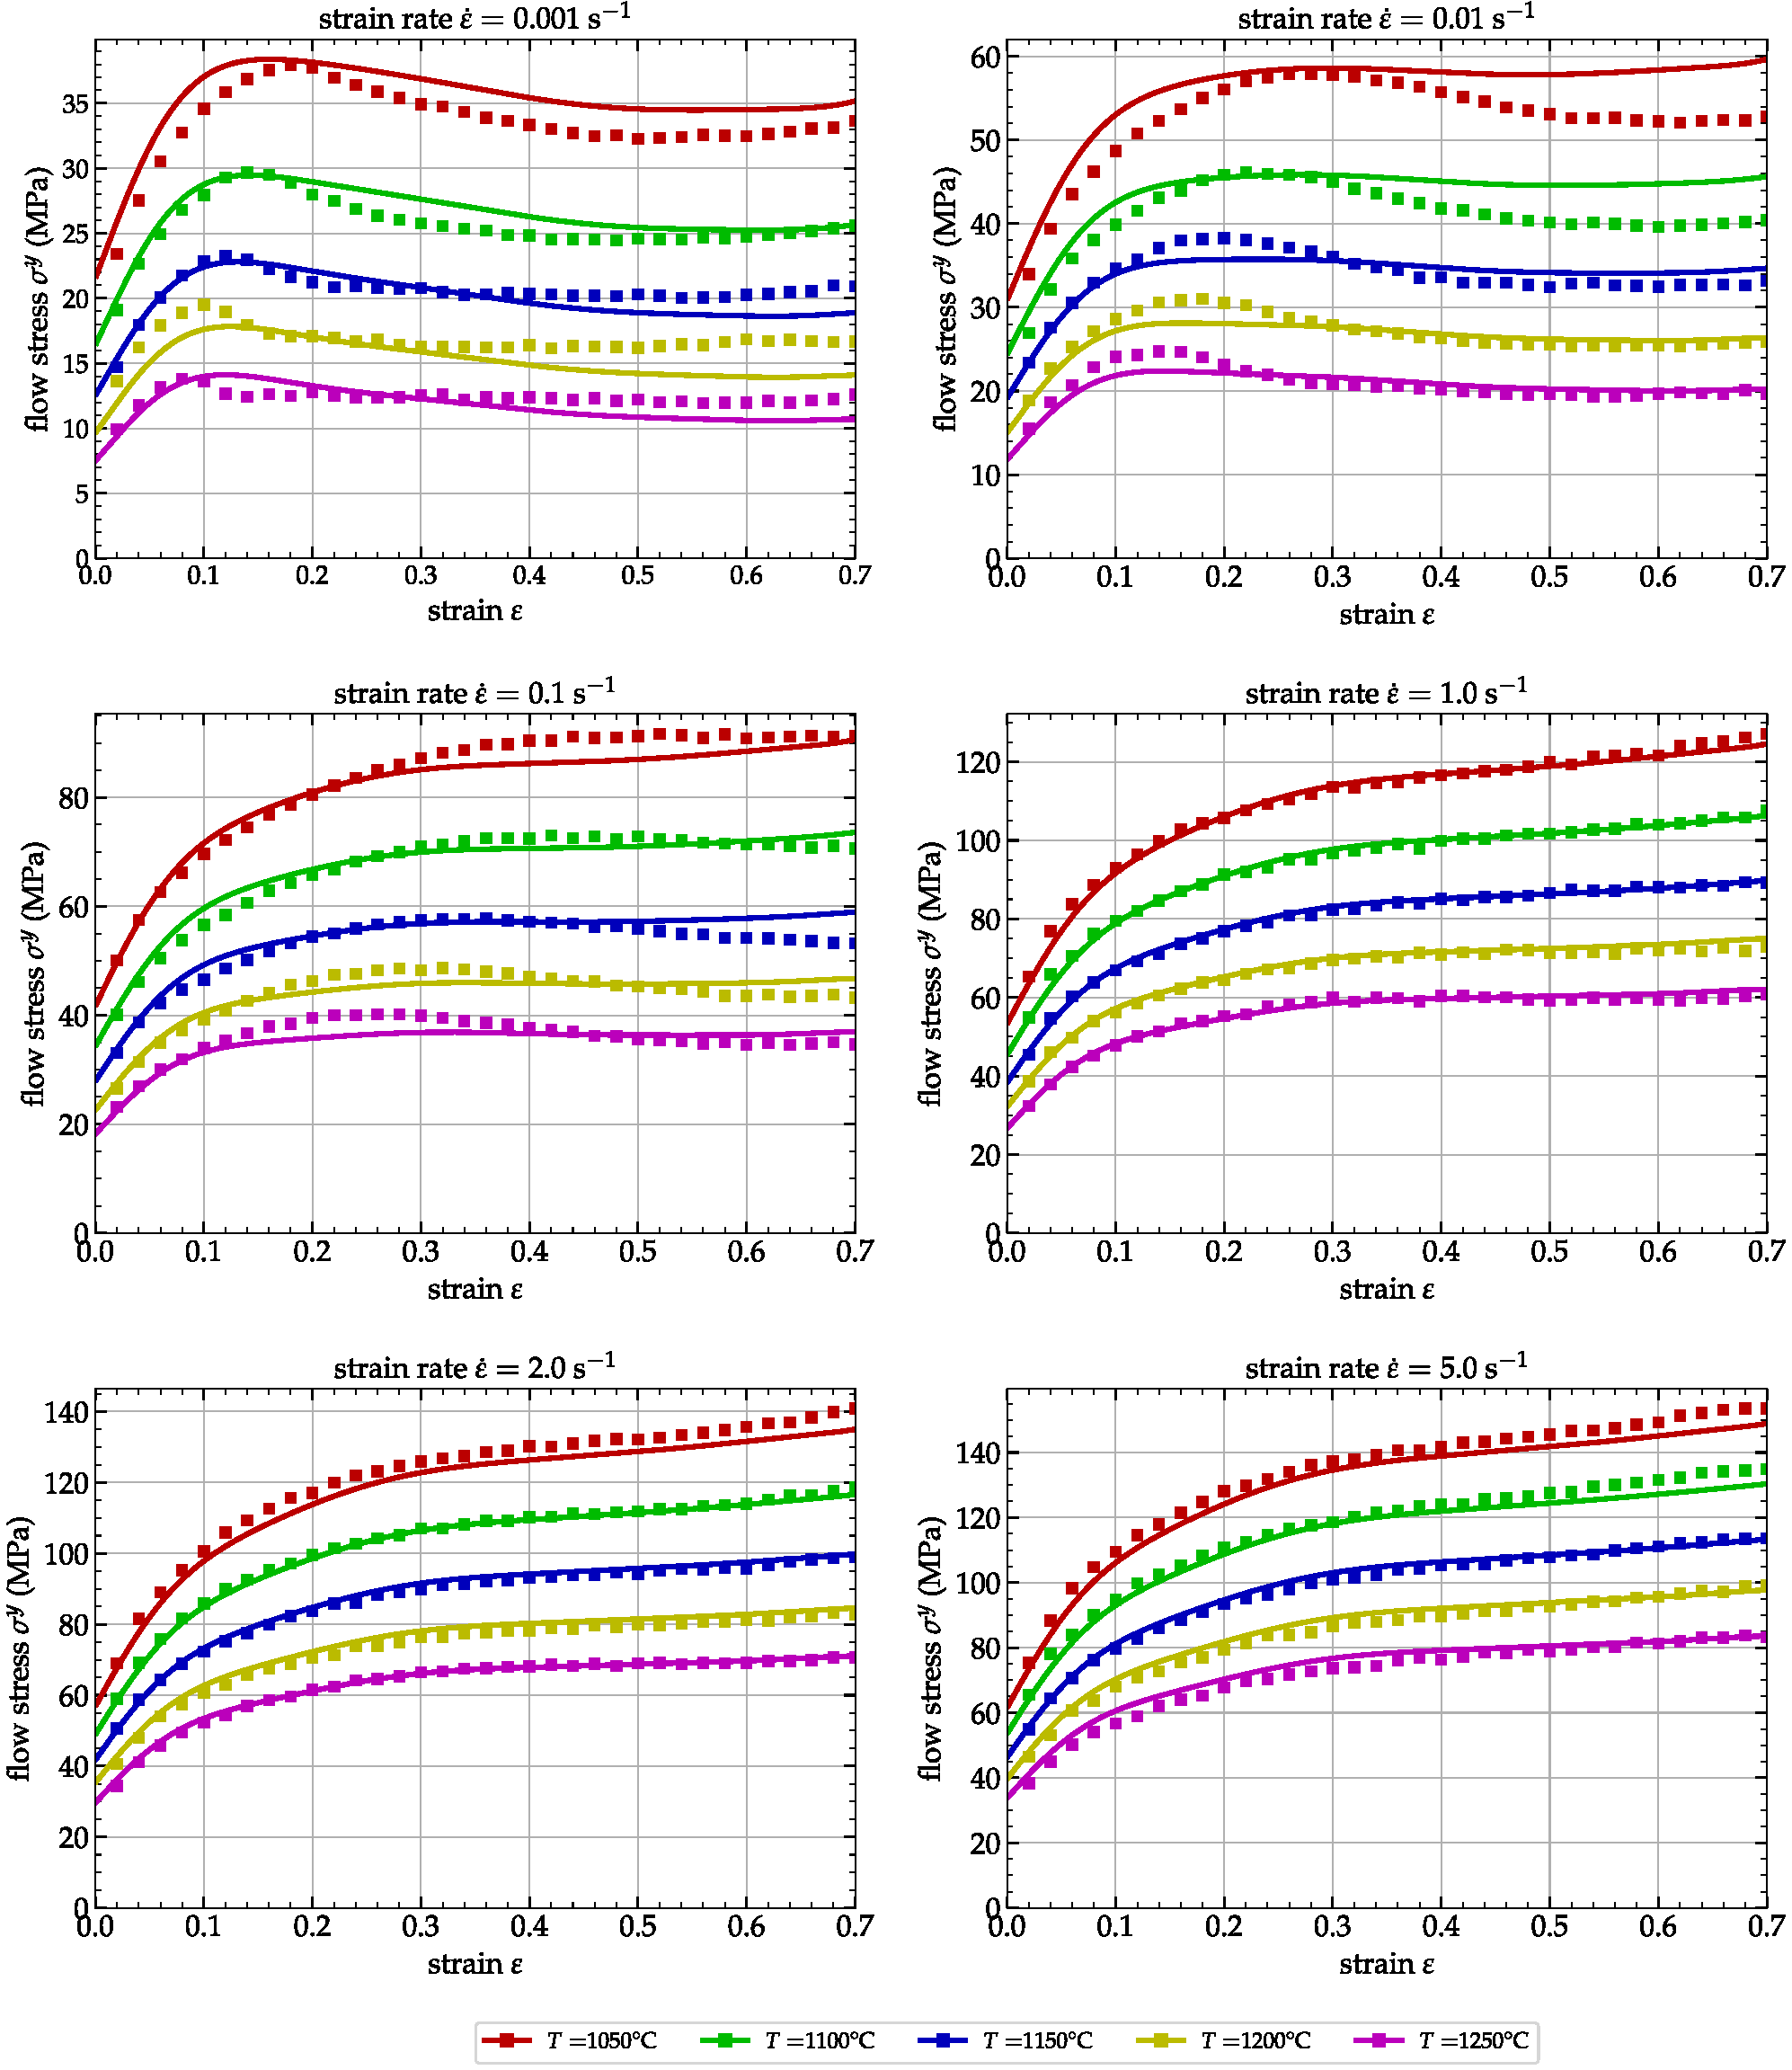
\includegraphics[width=0.98\columnwidth]
{Figures/CompExp-AR-6}
\caption{Comparison between the experimental (dots) and predicted (lines) flow stresses $\sigma^y$ by the Arrhenius model.}
\label{fig:CompExp-AR-6}
\end{figure}

Figure \ref{fig:CompExp-PTM-6} presents a comparison of the values predicted by the PTM model and the experimental values.
The PTM model is suitable for describing the flow behavior of medium carbon steel, but for the two strain rates $\mdot\varepsilon=0.01~\ps$ and $\mdot\varepsilon=0.1~\ps$, the prediction is not very good.
The deviation between the predicted values and the experimental values for other strain rates is relatively low.
For the PTM model, $\MARE=4.79\%$ and $\RMSE=4.59~\MPa$, which is an overall worse performance than the AR model.

\begin{table}[H]
\centering
\caption{Parameter values of the PTM flow law for the P20 steel.}
\newcolumntype{L}{>{\raggedright\arraybackslash}X}
\begin{tabularx}{\textwidth}{LLLL}
\toprule
\multicolumn{1}{c}{\boldmath{$A_i$}} & \multicolumn{1}{c}{\boldmath{$B_i$}} & \multicolumn{1}{c}{\boldmath{$C_0^i$}} & \multicolumn{1}{c}{\boldmath{$C_1^i$}} \\
\midrule
$A_0=16.8529$ & $B_0=-3.5418\times 10^{-3}$ & $C_0^0=0.1608$ & $C_1^0=-1.9037\times 10^{-5}$ \\
$A_1=340.6451$ & $B_1=-0.0132$ & $C_0^1=-0.6202$ & $C_1^1=2.67\times 10^{-3}$ \\
$A_2=-1.9594\times 10^{3}$ & $B_2=-4.4888\times 10^{-3}$ & $C_0^2=4.9516$ & $C_1^2=-3.5788\times 10^{-3}$ \\
$A_3=4.836\times 10^{3}$ & $B_3=0.2218$ & $C_0^3=-13.1694$ & $C_1^3=-0.0222$ \\
$A_4=-5.5176\times 10^{3}$ & $B_4=-0.4988$ & $C_0^4=15.25$ & $C_1^4=0.0609$ \\
$A_5=2.4058\times 10^{3}$ & $B_5=0.3211$ & $C_0^5=-6.587$ & $C_1^5=-0.0413$ \\
\bottomrule
\end{tabularx}
\label{tab:PTM}
\end{table}

\begin{figure}[H]

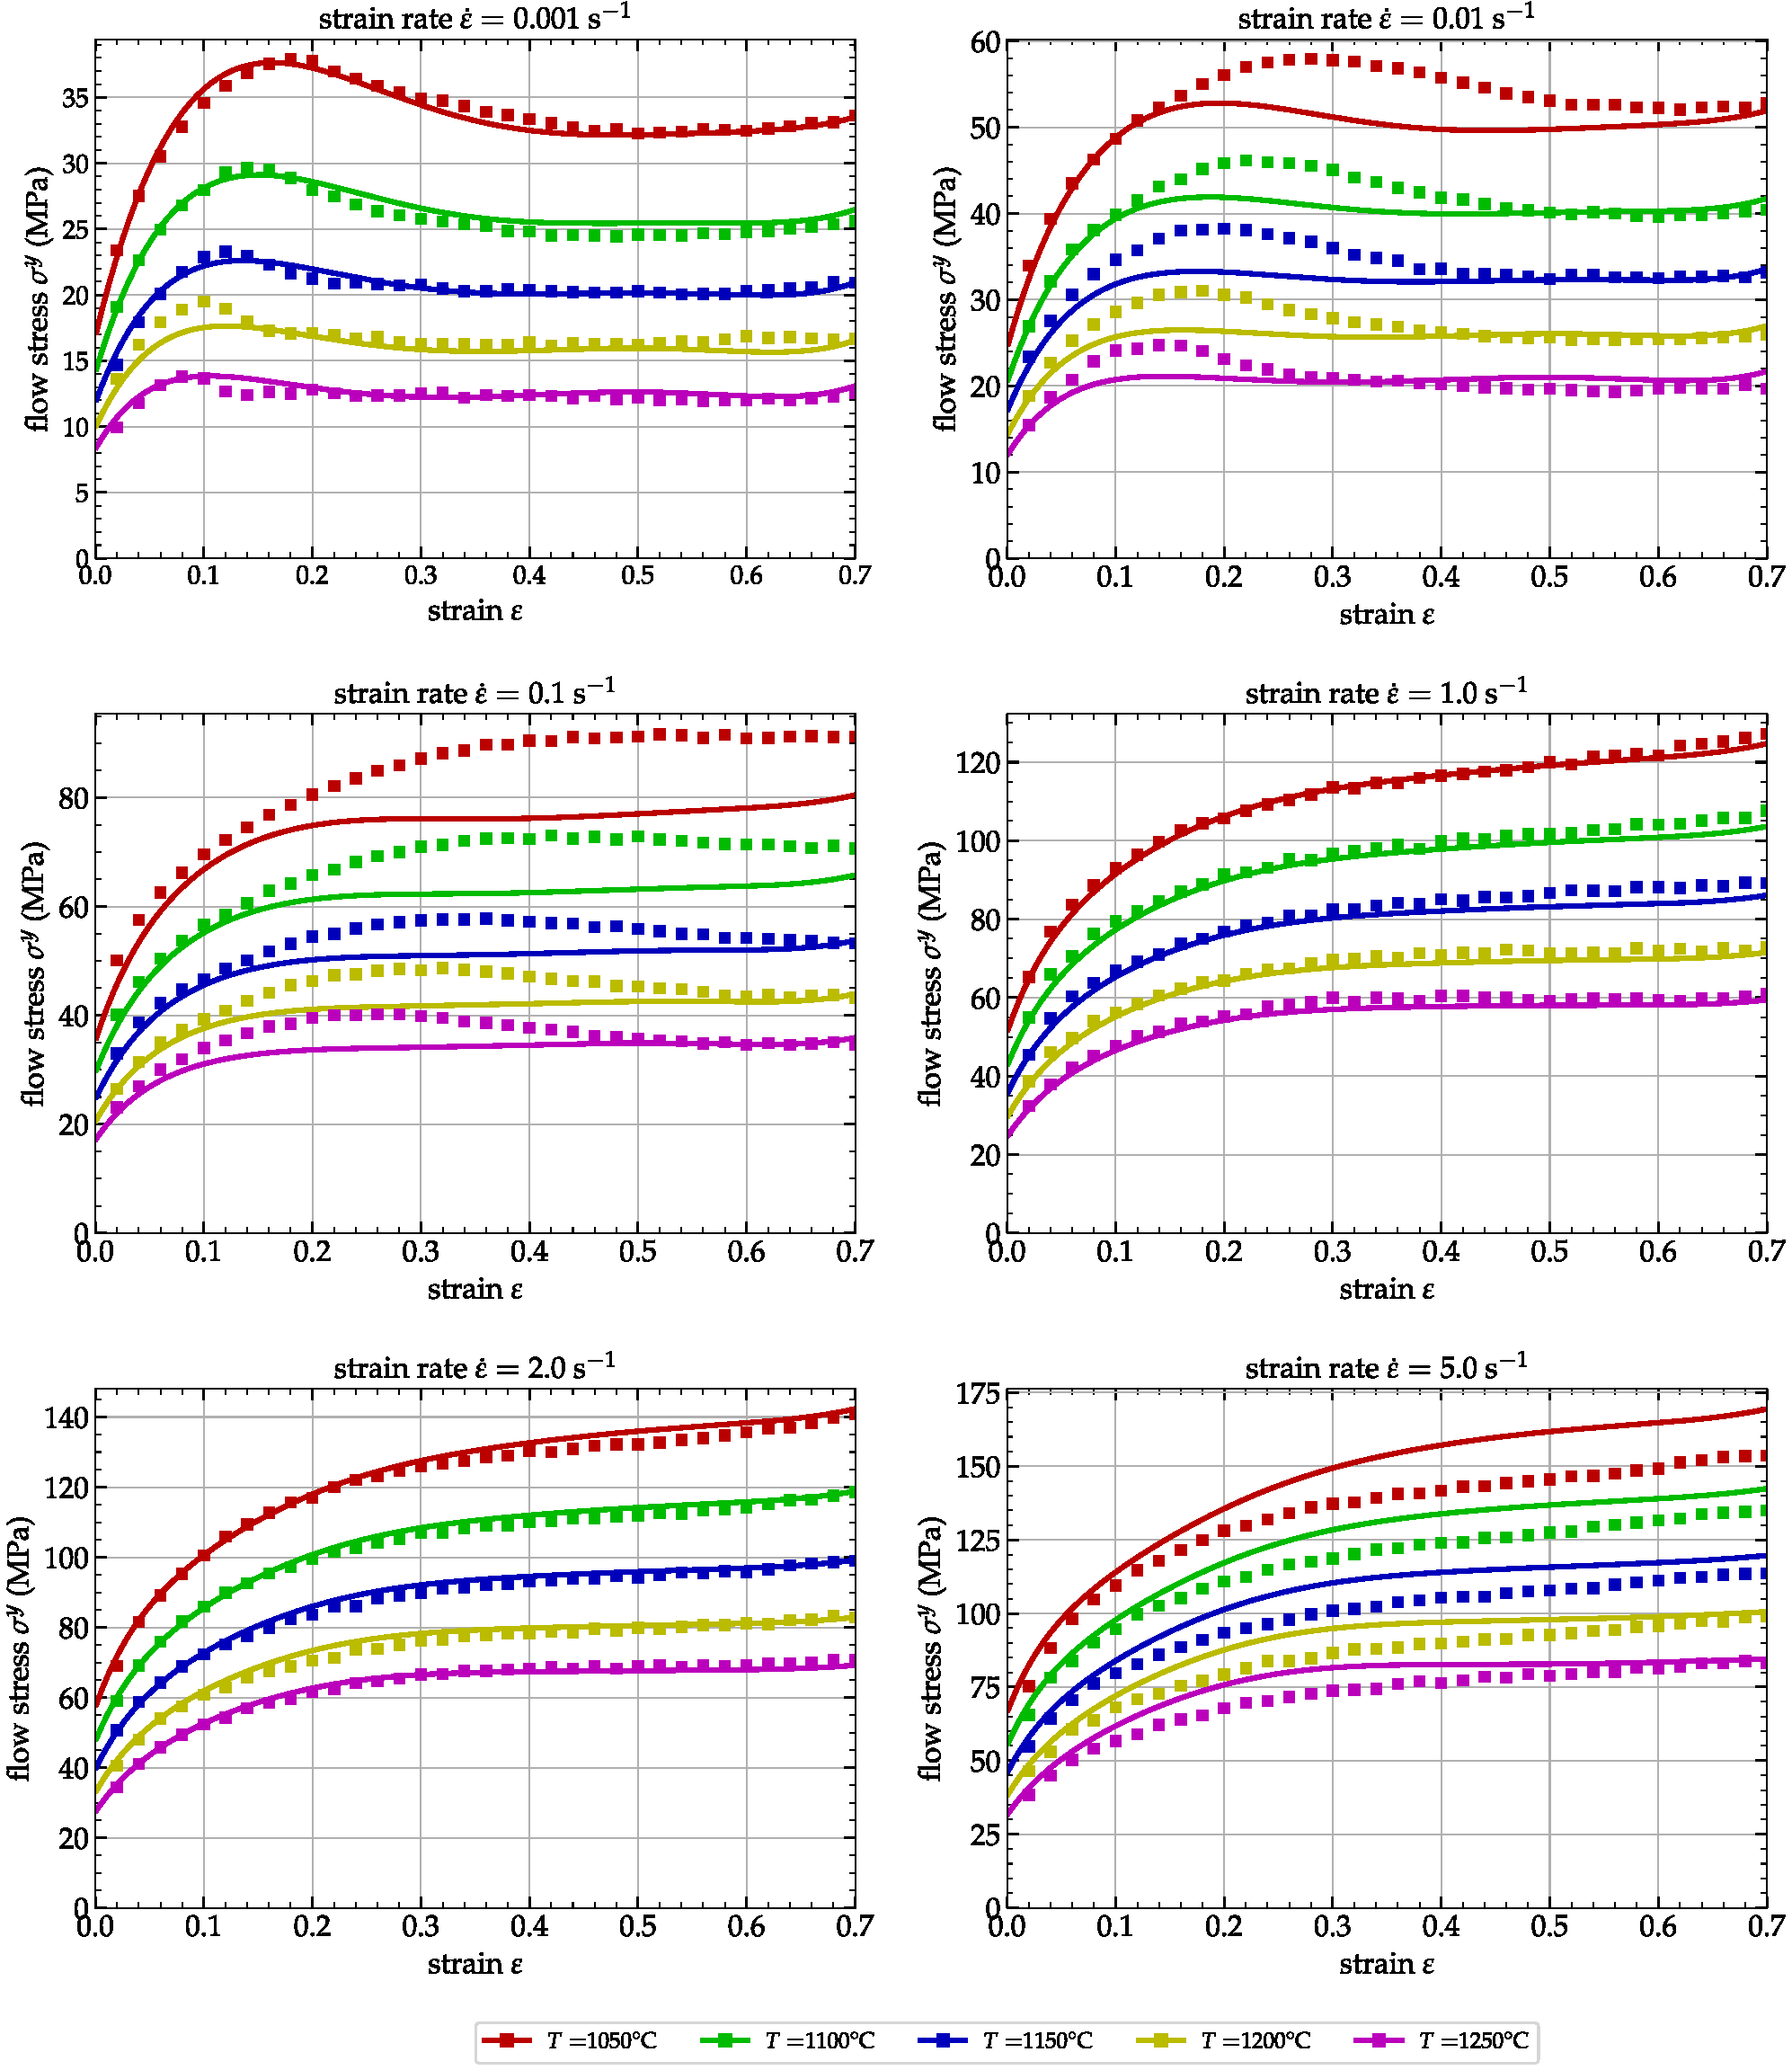
\includegraphics[width=0.98\columnwidth]
{Figures/CompExp-PTM-6}
\caption{Comparison between the experimental (dots) and predicted (lines) flow stresses $\sigma^y$ by the PTM model.}
\label{fig:CompExp-PTM-6}
\end{figure}

%----------------------------------------------------------------------------------
\subsection{The Artificial Neural Network Model\label{sec:ANNmodel}}
%----------------------------------------------------------------------------------

Because of their predictive capacity and adaptability, artificial neural networks (ANNs) are increasingly widely used today in many scientific fields.
Their operation is based on a training process, during which the principle of minimizing the error between the model's output and the training data allows the adjustment of the model's parameters, as in any machine training process.

Neural networks generally have two uses: classification and regression.
The first is the ability to classify data into different groups, for example to distinguish between images of cats and dogs.
The second corresponds to the universal approximation capacity of these neural networks, which is of interest to us herein, and thus, to the ability, after training, to predict the flow stress $\sigma^y$ values according to the input data, akin to what is achieved by the above-identified analytical models.
The main difference is that this approximation is not linked to a fixed mathematical formulation (as in the JC, MZA, AR, HS, and PTM analytical models), but is only dependent on the data used for training, the number of layers, the number of neurons per layer, and the activation functions associated with the neurons of the network.
A feed-forward ANN, as used in our application, contains an input layer, an output layer, and a number of hidden layers ($2$ in our case).
Each layer of neurons is connected to the one before it and the one after it by weighted connections.
Thus, all the neurons of the $k^{th}$ layer are connected to all the neurons of the ($k-1^{th}$) layer, as shown in~Figure~\ref{fig:ANN-2HL}.

\vspace{-2pt}
\begin{figure}[H]

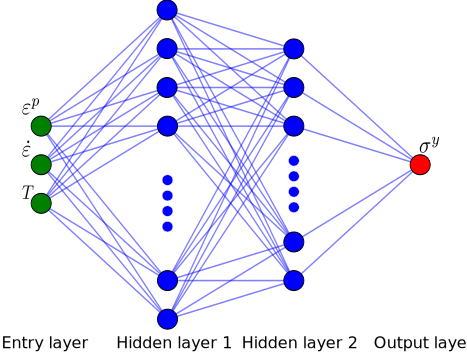
\includegraphics[width=0.7\columnwidth]
{Figures/ANN-scheme-2HL}
\caption{{Two} %MDPI: Should green and red dot be explained?. Caption modified.
 hidden layers artificial neural network architecture with 3 inputs neurons (green) and 1 output neuron (red).}
\label{fig:ANN-2HL}
\end{figure}

Any hidden layer $k$, containing $n$ neurons, takes a weighted sum of the outputs $\overrightarrow{\hat{y}}$ of the immediately preceding layer $(k-1)$, containing $m$ neurons, given by the following~equation:
\begin{equation}
y_i\lay{k} = \sum_{j=1}^m w_{ij}\lay{k} \hat{y}_j^{(k-1)}+ b_i\lay{k},\label{eq:ANN1}
\end{equation}
where $y_i\lay{k}$ is the entry of the  $i$th neuron of layer $k$, $\hat{y}_j\lay{k-1}$ is the output {of the} %MDPI: We suggest to remove the superscript and italic format of ``th''. Please check all the ``th''. Notation has been changed following your request.
  $j$th neuron of layer $(k-1)$, $w_{ij}\lay{k}$ is the associated weight parameter between the  $i$th neuron of layer $k$ and the  $j$th neuron of layer $(k-1)$, and $b_i\lay{k}$ is the associated bias of the  $i$th neuron of layer $k$.
Those weights $w_{ij}$ and bias $b_i$, for each layer, are the training parameters of the ANN, which we have to adjust during the training procedure described in Pantalé \eal \cite{Pantale-2021, Pantale-2023}.
For the proposed model, we selected the Sigmoid activation function, so that each neuron in the hidden layer $k$ provides an output value ${\hat{y}}$ from the input value $y$ of the same neuron defined by Equation (\ref{eq:ANN1}) according to the following equation:
\begin{equation}
\hat{y}=\frac{1}{1 + \e{-y}}\label{eq:ANN2}
\end{equation}

No activation function was used for the output neuron of the ANN as usually done in a regression ANN.

After some tests of different types of network architectures and in accordance with previous works, a network structure with two hidden layers including $15$ neurons for the first hidden layer and $7$ neurons for the second layer gave the best compromise between prediction, training time, and model compactness.
From a global architecture point of view, the input layer is composed of $3$ neurons ($\varepsilon^p$, $\mdot\varepsilon$, $T$) and the output layer is composed of a single neuron corresponding to the $\sigma^y$ flow stress.
This architecture leads to a global model with $180$ parameters to be identified ($60$ for the first layer, $112$ for the second layer, and $8$ for the output layer).

The Python program used for training the neural network was developed using the specialized Python library, Tensorflow \cite{Abadi-2016}.
The Adaptive Moment Estimation (ADAM) optimizer \cite{Kingma-2015} was used for the training phase.
The training data were those from the tests presented in Section \ref{sec:ComTestResults} and were composed of 21,000 quadruplets of ($\varepsilon^p$, $\mdot\varepsilon$, $T$, $\sigma^y$) values.
The training was performed on the basis of $5000$ epochs of the experimental dataset.
It took $40$~min of training on a Dell XPS-13 7390 laptop running Ubuntu 22.04 LTS 64 bits with 16~GB of RAM and an Intel 4-core i7-10510U processor to obtain the converged parameters of the ANN model.
Figure \ref{fig:ANN-6-conv} shows the evolution of the training error defined by the $\log_{10}$ of the $\RMSE$ during the training phase.
\begin{figure}[H]
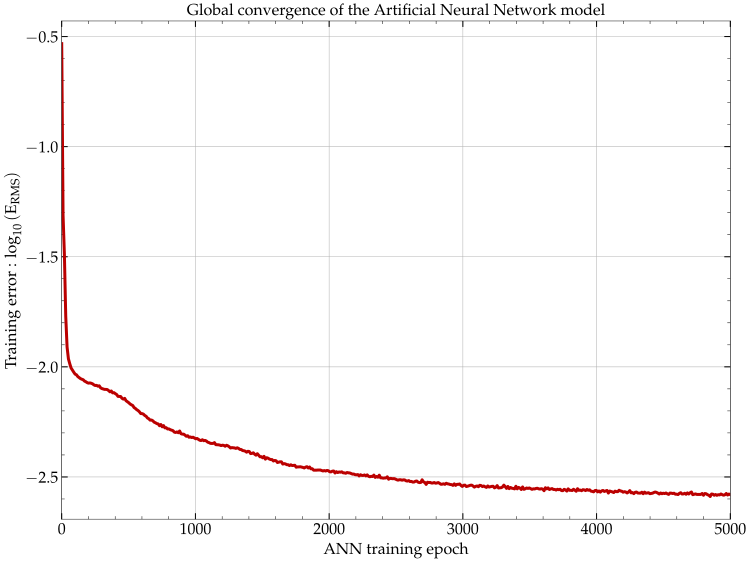
\includegraphics[width=0.7\columnwidth]
{Figures/Conv-ANN-6}
\caption{Convergence of the ANN model during the training phase.}
\label{fig:ANN-6-conv}
\end{figure}
As can be seen in this figure, after $5000$ epochs, we can consider that we have reached a stationary state of the model training, such that it is useless to continue with the training~phase.

\textls[-25]{Once the training phase is over, the trained model can be used to predict the behavior of the medium carbon alloy as a function of the input data, similarly to what was done with the analytical models.
One can either use the model directly by providing it with new input data or retrieve the $180$ parameters identified during the training and inject them into a mathematical model based on Equations (\ref{eq:ANN1}) and (\ref{eq:ANN2}), which can be implemented in any language (\eg in FORTRAN for use on the Abaqus Explicit FEA code), as proposed in Pantalé \eal \cite{Pantale-2021, Pantale-2023}.
For compactness, the parameters of the ANN model and the complete procedure to compute the flow stress $\sigma^y$ from the input data are provided in {Appendix} %MDPI: We changed Appendix to Appendix A. OK
 \ref{sec:Appendix}.}

As for the above-considered analytical models, Figure \ref{fig:CompExp-3-15-7-1-sigmoid} shows a comparison between the flow stresses predicted by the ANN model and the data measured during the hot compression test.

The experimental data and the ANN prediction correlate very well over the entire range of data, and the predicted data can track the hardening and softening regions of the hot deformed material well.
For the ANN model, $\MARE=0.62\%$ and $\RMSE=0.38~\MPa$, which is excellent.
This model can be used to simulate the hot deformation of this type of alloy with much greater reliability with respect to the actual material behavior than the analytical models presented in the above sections.


\begin{figure}[H]

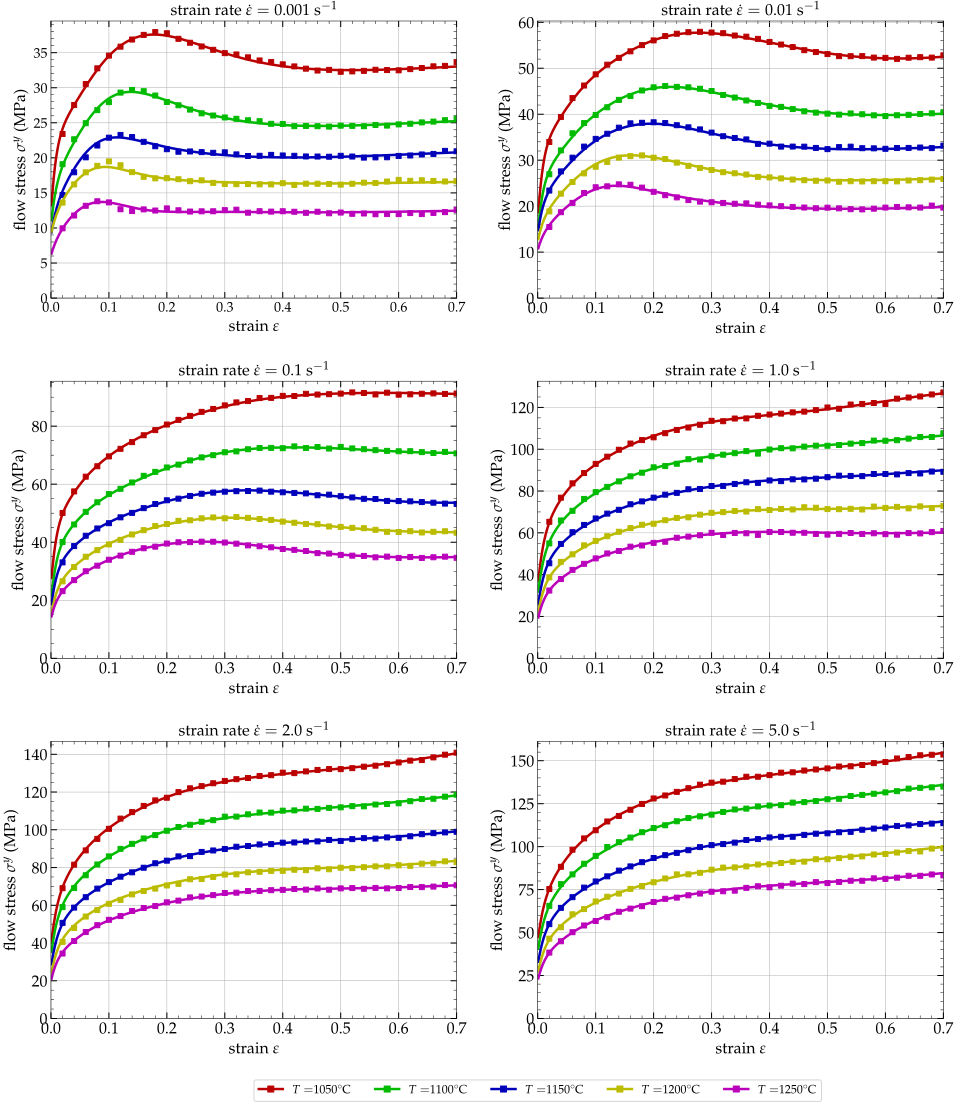
\includegraphics[width=0.98\columnwidth]
{Figures/CompExp-3-15-7-1-sigmoid}
\caption{Comparison between the experimental (dots) and predicted (lines) flow stresses $\sigma^y$ by the 3-15-7-1-sigmoid ANN model.}
\label{fig:CompExp-3-15-7-1-sigmoid}
\end{figure}

%----------------------------------------------------------------------------------
\subsection{Comparison of Analytical and ANN Models\label{sec:Comparison}}
%----------------------------------------------------------------------------------

A summary of the coefficients for evaluating the high-temperature flow stress prediction capability of the medium carbon alloy for all models presented in this work is reported in Table \ref{tab:Errors}.
\begin{table}[H]

\caption{Accuracy coefficients for all the analyzed models.}
\newcolumntype{C}{>{\centering\arraybackslash}X}
\newcolumntype{L}{>{\raggedright\arraybackslash}X}
\begin{tabularx}{\textwidth}{LCCCCCC}
\toprule
\textbf{Coefficients} & \textbf{JC} & \textbf{MZA} & \textbf{HS} & \textbf{AR} & \textbf{PTM} & \textbf{ANN} \\
\midrule
$\MARE(\%)$ & $14.05$ & $21.20$ & $7.75$ & $3.56$ & $4.79$ & $0.62$ \\
$\RMSE(\MPa)$ & $12.00$ & $19.57$ & $3.80$ & $2.18$ & $4.59$ & $0.38$ \\
\bottomrule
\end{tabularx}
\label{tab:Errors}
\end{table}
From Table \ref{tab:Errors}, we can see that the ANN model has a much better predictive capacity than all the analytical models presented in the above sections.
Globally, the values of $\MARE$ and $\RMSE$ are six-times lower than with the best of the analytical models, \ie the Arrhenius model, quoted as reference in the context of the hot forming of alloys \cite{Liang-2022}.

The ANN, Arrhenius and PTM models are the only models that take into account softening with the deformation of medium carbon at a low strain rate, unlike the other three models, which only present an increase in the flow stress with the strain, irrespective of the strain rate and temperature, hence their poor performance in predicting the behavior of this material and, more particularly, at low strain rates.
The parameters reported in \mbox{Table \ref{tab:Errors}} and the correlations that can be seen in Figures \ref{fig:CompExp-JC-6}{--}%MDPI: We changed ``to'' to en dash. OOPS, there is a mistake, it's figures 6,7,8,9,10, and 13. Figures 11 and 12 cannot be included in this list. I updated the cross references.
\ref{fig:CompExp-PTM-6} and \ref{fig:CompExp-3-15-7-1-sigmoid} allow concluding that the ANN model is the most efficient of all the models presented when it comes to describing the behavior of the medium carbon alloy for high-temperature deformation applications.

%----------------------------------------------------------------------------------
\section{Interpolation and Extrapolation Capability of Models\label{sec:IntExt}}
%----------------------------------------------------------------------------------

In order to better compare the performances of the above analyzed models (the five~analytical models and the ANN based model), in this section, we present the ability of each of these models to interpolate and extrapolate the results as a function of the strain rate $\mdot\varepsilon$.
The identification of the above-analyzed models was based on a set of experimental data corresponding to six strain rates, five temperatures, and strains ranging from $0$ to $0.7$.
To test the training capacity and reliability of these models, we propose here to perform the training of the models on only five strain rates by voluntarily omitting the strain rate $\mdot\varepsilon=1~\ps$ or $\mdot\varepsilon=5~\ps$.

Thus, one of the omitted strain rates ($\mdot\varepsilon=1~\ps$) is within the range of strain rates for model identification ($0.001~\ps\text{ to }5~\ps$), and therefore, we can test the ability of the models to interpolate the results from the other five strain rates and be able to quantify any deviation from experimental values.
On the other hand, since the omitted strain rate ($\mdot\varepsilon=5~\ps$) is outside the range of strain rates for the model identification ($0.001~\ps\text{ to }2~\ps$), we tested the ability of the models to extrapolate the results and quantify deviations with the experimental values.

%----------------------------------------------------------------------------------
\subsection{Interpolation Validation}
%----------------------------------------------------------------------------------

For interpolation validation, the chosen omitted strain rate was $\mdot\varepsilon=1~\ps$, and \linebreak those used for identification (or training for the ANN) were the five others, \ie \linebreak \mbox{$\mdot\varepsilon=[0.001, 0.01, 0.1, 2, 5]~\ps$}.
All models were re-identified from the same experimental data on a dataset corresponding to five strain rates and five temperatures.

Figure \ref{fig:CompInt} shows a comparison, for the strain rate $\mdot\varepsilon=1~\ps$, of the flow stresses $\sigma^y$ calculated by the models (as a line) and the experimental results (as dots) for the five analytical models and the neural network.

Table \ref{tab:IntVal} shows the $\MARE$ and $\RMSE$ deviations between the different models and the experimental data calculated either for the five identified strain rates (lines referred as id. $\mdot\varepsilon$), the six strain rates (lines referred as all $\mdot\varepsilon$), or only on the strain rate $\mdot\varepsilon=1~\ps$.

\vspace{-2pt}
\begin{table}[H]
\centering{}
\caption{Accuracy coefficients of interpolation for all models with $\mdot\varepsilon=1~\ps$.}

\begin{adjustwidth}{-\extralength}{0cm}
%\centering %% If there is a figure in wide page, please release command \centering
\begin{minipage}{\fulllength}
\newcolumntype{C}{>{\centering\arraybackslash}X}
\newcolumntype{L}{>{\raggedright\arraybackslash}X}
\begin{tabularx}{\textwidth}{LLCCCCCC}
\toprule
\textbf{Strain Rate} & \textbf{Coefficients} & \textbf{JC} & \textbf{MZA} & \textbf{HS} & \textbf{AR} & \textbf{PTM} & \textbf{ANN} \\
\midrule
\mr{2}{id. $\mdot\varepsilon$} & $\MARE(\%)$ & $13.79$ & $20.22$ & $8.57$ & $3.96$ & $5.10$ & $0.70$ \\
& $\RMSE(\MPa)$ & $11.83$ & $19.00$ & $3.97$ & $2.29$ & $4.73$ & $0.38$ \\
\midrule
\mr{2}{$\mdot\varepsilon=1~\ps$} & $\MARE(\%)$ & $14.87$ & $27.79$ & $3.74$ & $1.46$ & $3.16$ & $2.47$ \\
& $\RMSE(\MPa)$ & $12.02$ & $23.67$ & $3.10$ & $1.46$ & $2.65$ & $2.77$ \\
\midrule
\mr{2}{all $\mdot\varepsilon$} & $\MARE(\%)$ & $14.42$ & $28.90$ & $7.55$ & $3.45$ & $4.90$ & $0.96$ \\
& $\RMSE(\MPa)$ & $11.86$ & $19.86$ & $3.84$ & $2.17$ & $4.45$ & $1.18$ \\
\bottomrule
\end{tabularx}
\end{minipage}
\end{adjustwidth}
\label{tab:IntVal}
\end{table}


\begin{figure}[H]

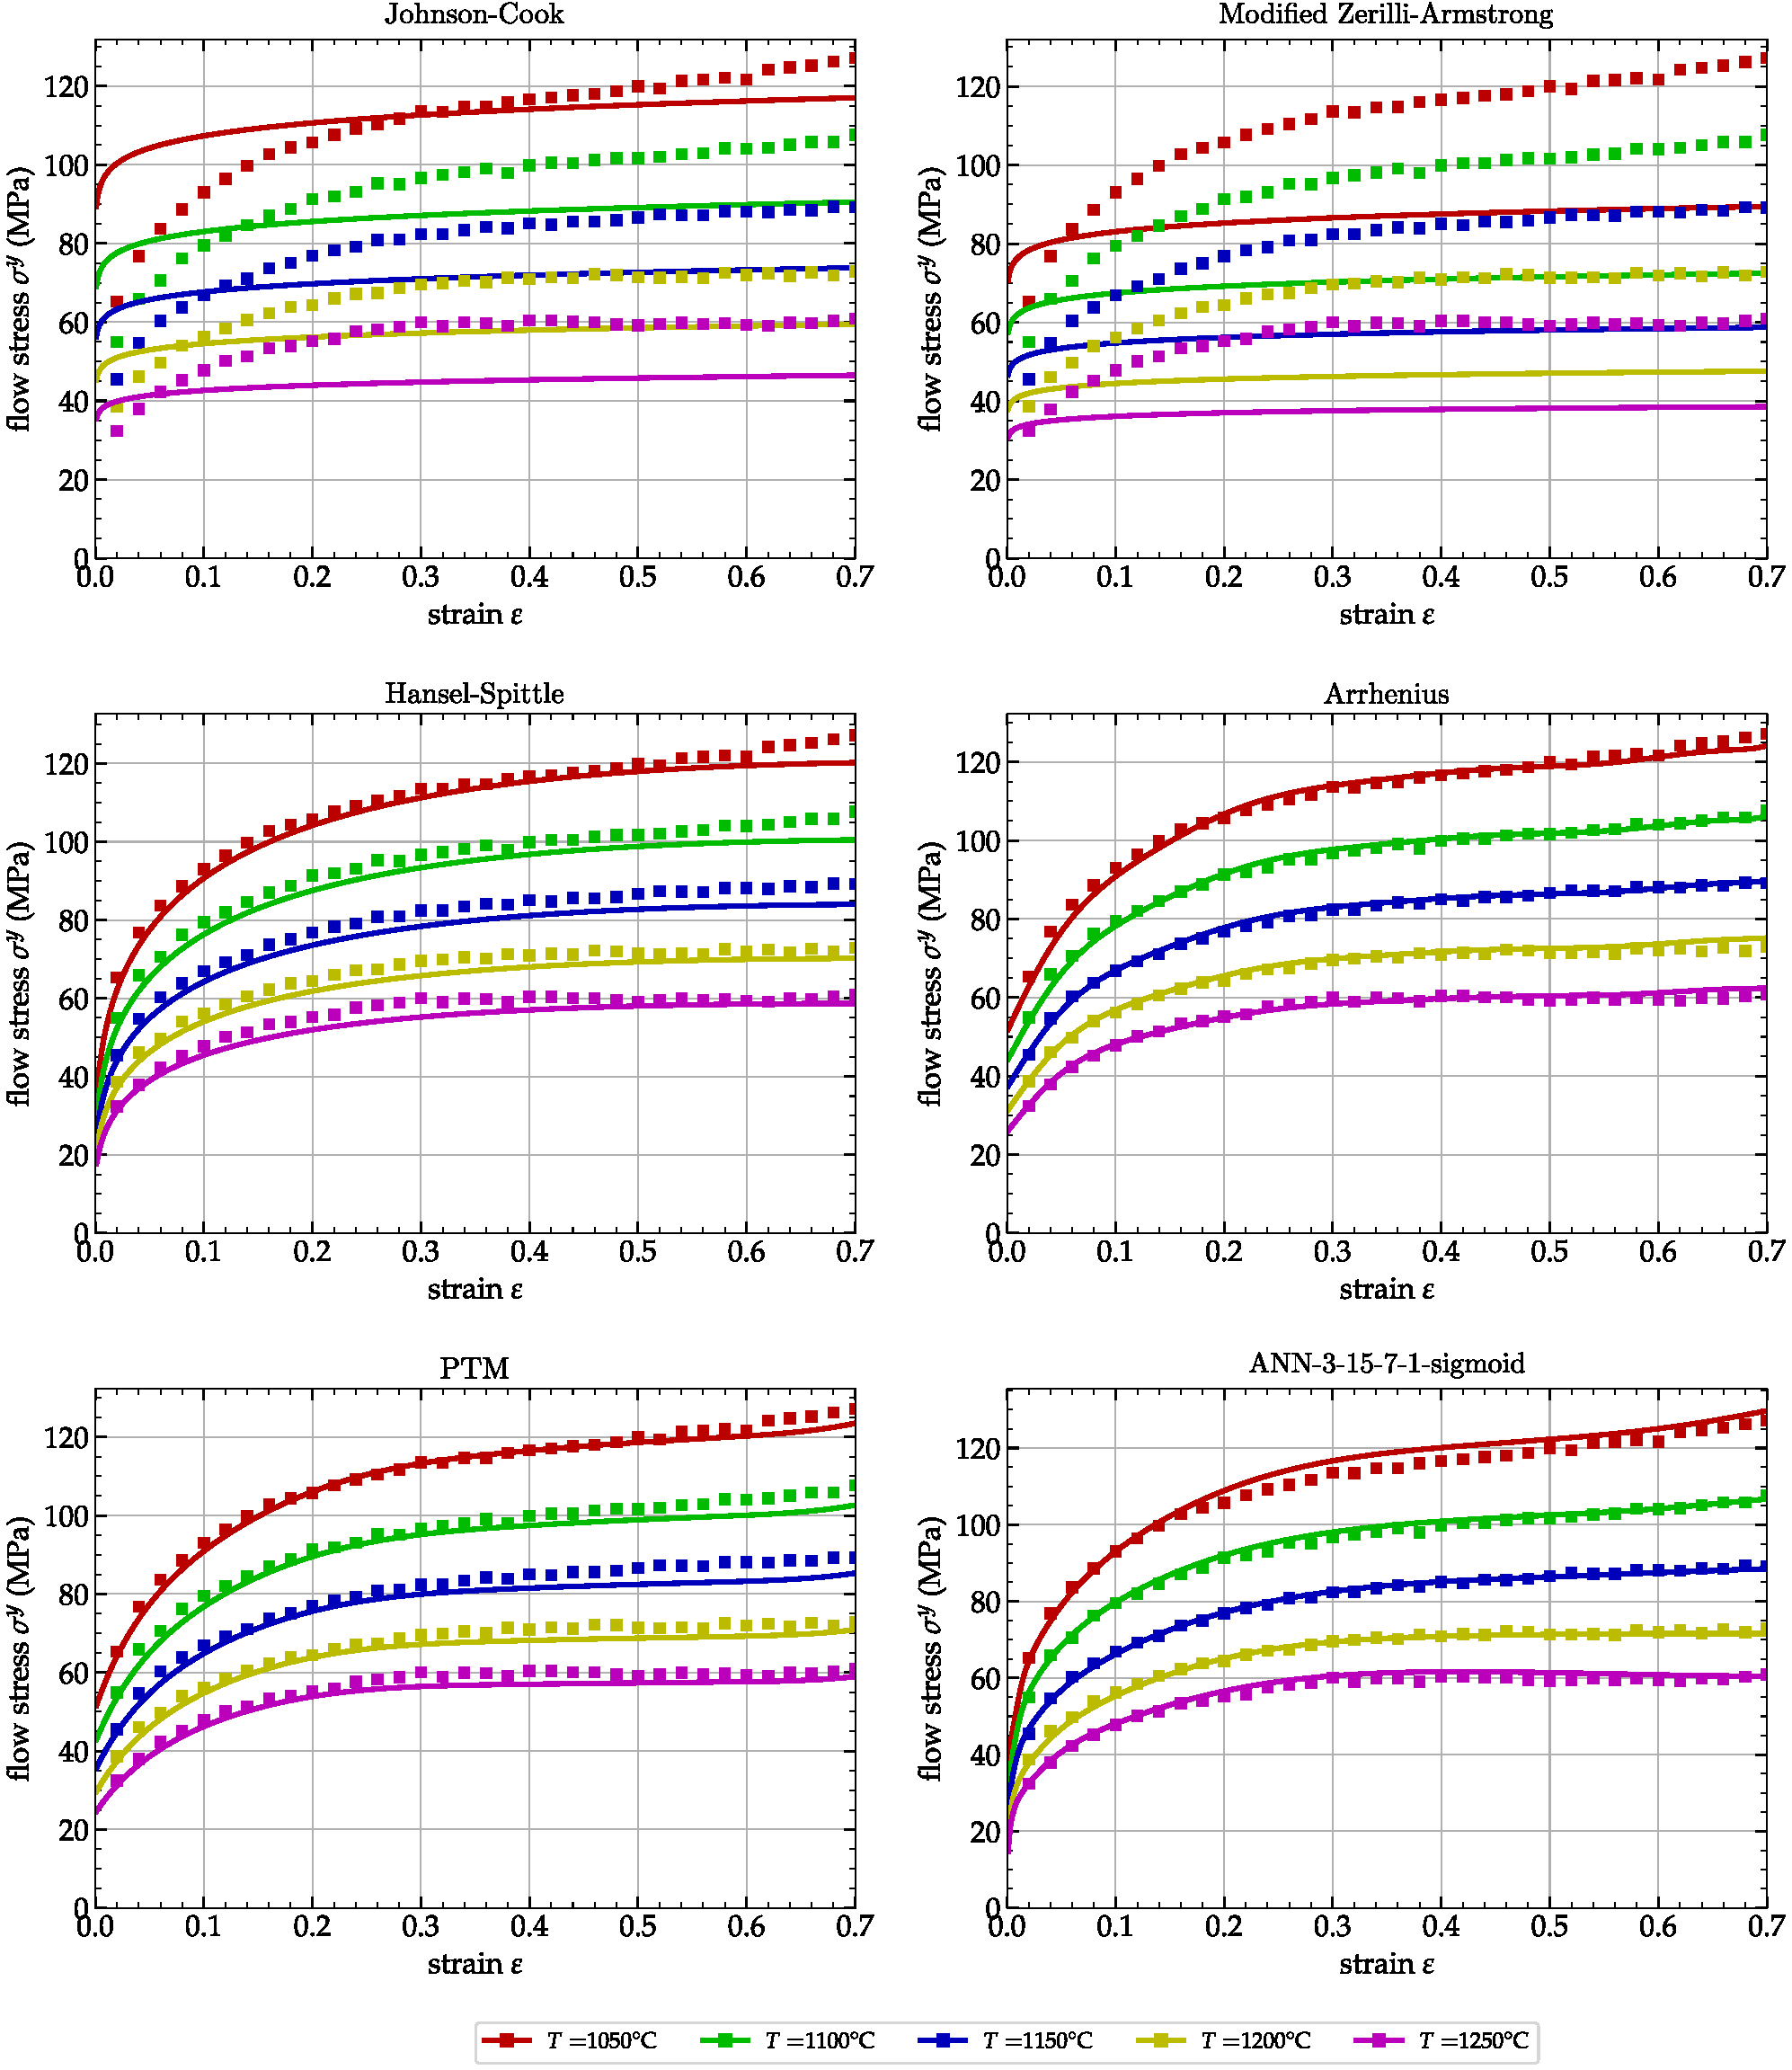
\includegraphics[width=0.98\columnwidth]
{Figures/CompInt}
\caption{Comparison between the experimental (dots) and predicted (lines) flow stresses $\sigma^y$ for $\mdot\varepsilon=1~\ps$.}
\label{fig:CompInt}
\end{figure}

In Figure \ref{fig:CompInt}, it can be seen that the first two models (JC and MZA) presented in this study do not have the ability to reproduce the behavior of the material for the strain rate $\mdot\varepsilon=1~\ps$.
Overall, the JC model gives better results than the MZA model for $\mdot\varepsilon=1~\ps$, which is reflected in Table \ref{tab:IntVal} by a lower value of the $\MARE$ and $\RMSE$ for the JC than for the MZA model.
Nevertheless, these values are higher than $10\%$ for the JC model and $20\%$ for the MZA model, which reflects the poor ability of these models to correctly model the behavior of this material.
This finding is in agreement with the previous findings of \mbox{Sections \ref{sec:JC} and \ref{sec:MZA}}, which showed the inability of these models to take into account the softening of the behavior visible at low strain rates and low temperatures.

From a general appearance point of view, the other four models, HS, AR, PTM, and ANN, give globally similar results, with a higher reliability for the AR and ANN models compared to the other two models.
Table \ref{tab:IntVal} shows a quantitative comparison of the $\MARE$ and $\RMSE$ for three different cases: the 5 identified strain rates, only the strain rate $\mdot\varepsilon=1~\ps$, and all 6 strain rates for these six models.
It appears from this table that, while the two models, AR and ANN, give equivalent (and excellent) results concerning the values of the $\MARE$ and $\RMSE$ for the strain rate $\mdot\varepsilon=1~\ps$, the ANN model gives a globally better result across the entire strain rate spectrum, with values of $\MARE=0.96\%$ and $\RMSE=1.18~\MPa$, respectively, that is to say, values that are approximately 2- to 3-times lower for the ANN model than for the AR model.

This shows the superior reliability of the ANN model over the five analytical models presented in this study both in terms of the interpolation capability of the model and of the overall behavior.

%----------------------------------------------------------------------------------
\subsection{Extrapolation Validation}
%----------------------------------------------------------------------------------

For the validation of the models' ability to extrapolate, the omitted strain rate chosen was $\mdot\varepsilon=5~\ps$ and those used for identification were $\mdot\varepsilon=[0.001, 0.01, 0.1, 1, 2]~\ps$.
The strain rate omitted in this analysis, therefore, has the highest value, which restricts the training~domain.

In this new identification configuration, Figure \ref{fig:CompExt} shows a comparison, for strain rate $\mdot\varepsilon=5~\ps$, of the flow stresses $\sigma^y$ computed by the models (as a line) and the experimental results (as dots) for the five analytical models and the neural network.
\begin{figure}[H]

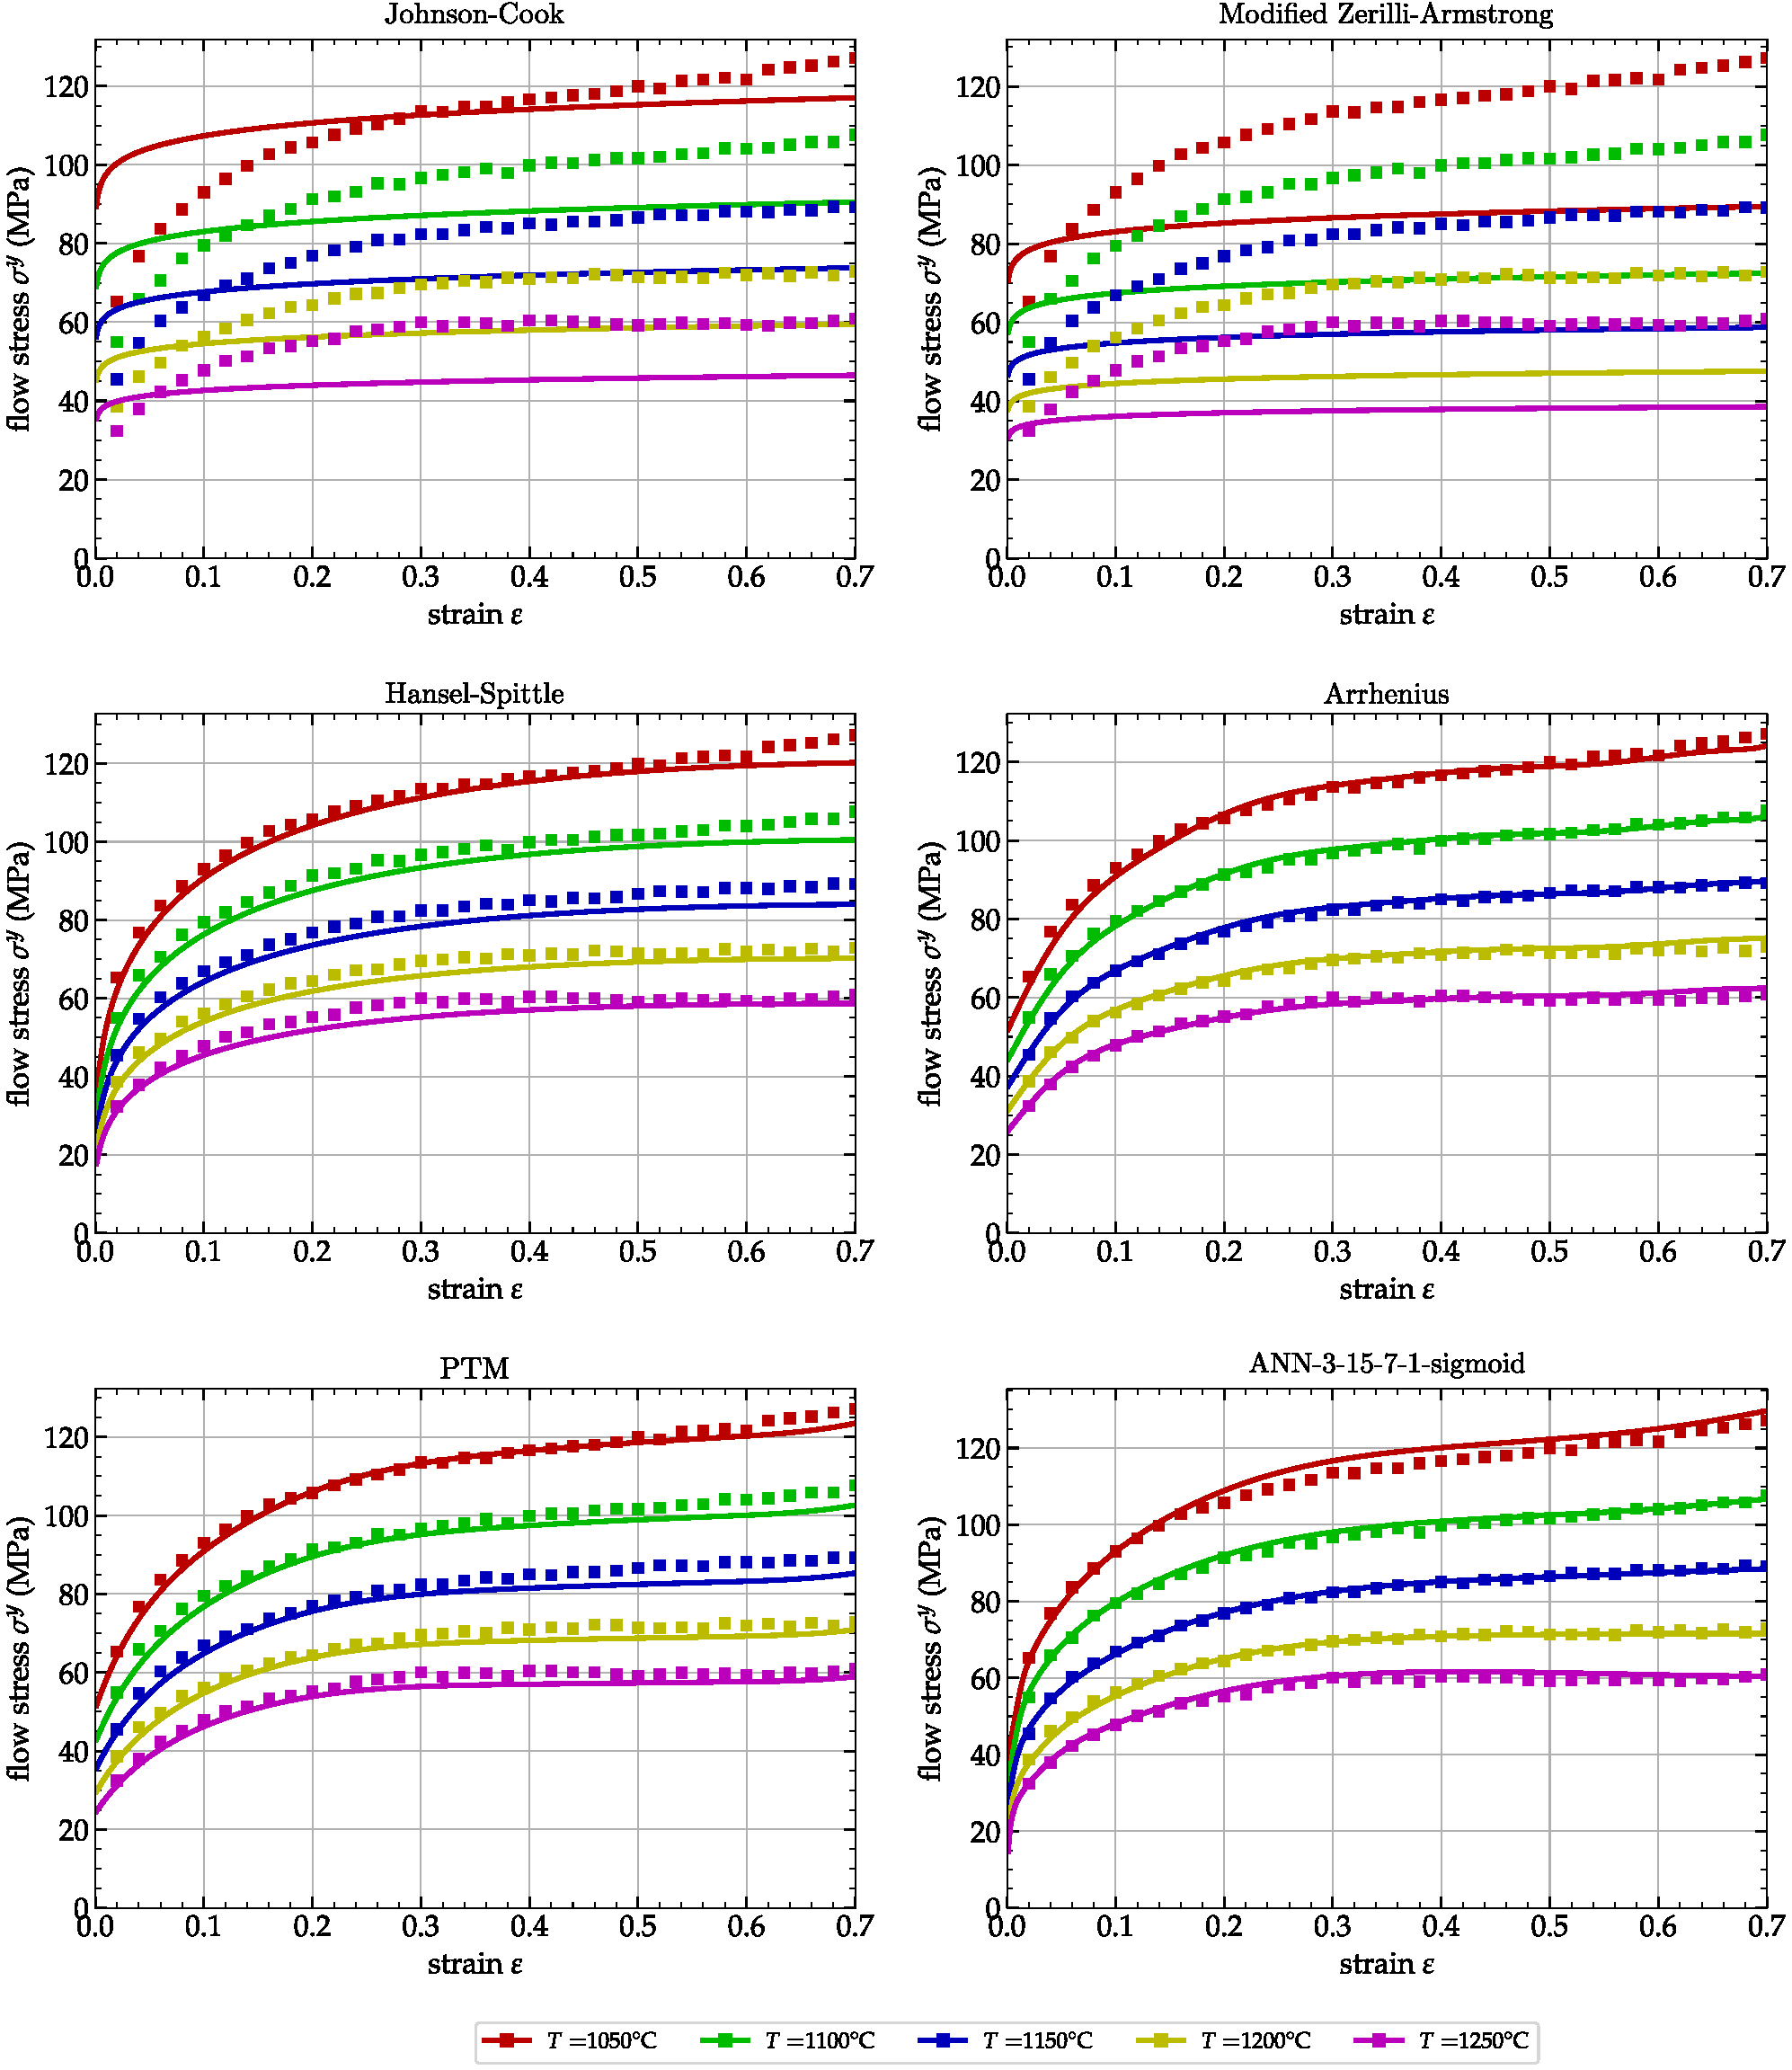
\includegraphics[width=0.98\columnwidth]
{Figures/CompExt}
\caption{{Comparison} %MDPI: Should hyphen be changed to en dash in 3-15-7-1?. No, since, this will lead to longuer notations, I have used hyphen instead of en dash to reduce the width of the notation ANN-3-15-7-1-sigmoid for the model.
 between the experimental (dots) and predicted (lines) flow stresses $\sigma^y$ for $\mdot\varepsilon=5~\ps$.}
\label{fig:CompExt}
\end{figure}
Table \ref{tab:ExtVal} shows the $\MARE$ and $\RMSE$ deviations between the different models and the experimental data calculated either for the $5$ identified strain rates (lines referred as id. $\mdot\varepsilon$), the $6$ strain rates (lines referred as all $\mdot\varepsilon$), or only on the strain rate $\mdot\varepsilon=5~\ps$.
\begin{table}[H]

\caption{Accuracy coefficients of extrapolation for all models with $\mdot\varepsilon=5~\ps$.}
\newcolumntype{C}{>{\centering\arraybackslash}X}
\newcolumntype{L}{>{\raggedright\arraybackslash}X}
\begin{tabularx}{\textwidth}{LLCCCCCC}
\toprule
\textbf{Strain Rate} & \textbf{Coefficients} & \textbf{JC} & \textbf{MZA} & \textbf{HS} & \textbf{AR} & \textbf{PTM} & \textbf{ANN} \\
\midrule
\mr{2}{id. $\mdot\varepsilon$} & $\MARE(\%)$ & $13.09$ & $19.09$ & $7.30$ & $4.03$ & $4.34$ & $0.61$ \\
& $\RMSE(\MPa)$ & $9.86$ & $16.26$ & $3.36$ & $2.32$ & $3.63$ & $0.32$ \\
\midrule
\mr{2}{$\mdot\varepsilon=5~\ps$} & $\MARE(\%)$ & $20.16$ & $24.27$ & $7.73$ & $3.53$ & $11.46$ & $3.87$ \\
& $\RMSE(\MPa)$ & $20.73$ & $25.95$ & $7.83$ & $4.02$ & $12.91$ & $5.84$ \\
\midrule
\mr{2}{all $\mdot\varepsilon$} & $\MARE(\%)$ & $15.12$ & $25.87$ & $7.12$ & $3.86$ & $5.34$ & $1.09$ \\
& $\RMSE(\MPa)$ & $12.36$ & $18.24$ & $4.43$ & $2.68$ & $6.23$ & $2.40$ \\
\bottomrule
\end{tabularx}
\label{tab:ExtVal}
\end{table}

As presented in the previous section regarding the interpolation capability of the models, in Figure \ref{fig:CompExt}, it can be seen that the first two models, JC and MZA, in this study again do not have the ability to correctly reproduce the material behavior for the strain rate \mbox{$\mdot\varepsilon=5~\ps$}.
The JC model performs better than the MZA model for $\mdot\varepsilon=5~\ps$, which is reflected in Table \ref{tab:ExtVal} by a lower value of the $\MARE$ and $\RMSE$ for JC than for MZA.
Nevertheless, these values are too large for proper use.
Once again, it is the inability of these models to take into account the softening of the behavior at low strain rates and low temperatures that is at the origin of these values.

The other four models, HS, AR, PTM, and ANN, give better results with higher reliability for the AR and ANN models than for the other two models.
Table \ref{tab:ExtVal} shows a comparison over all strain rates and over $\mdot\varepsilon=5~\ps$ for these six models.
The HS model performs worse in extrapolation than the AR and ANN models, while the PTM model is relegated to the last position in this ranking with values of the $\MARE$ and $\RMSE$ greater than $10\%$ for the strain rate $\mdot\varepsilon=5~\ps$.
The two models, AR and ANN, give the best results for the values of the $\MARE$ and $\RMSE$ for the strain rate $\mdot\varepsilon=5~\ps$.
This time, the AR model performs a little better on the $\mdot\varepsilon=5~\ps$ strain rate as compared to the ANN model, but the latter gives a globally better result across the entire strain rate spectrum, with values of $\MARE=1.09\%$ and $\RMSE=2.40~\MPa$, respectively.

We can, therefore, conclude from this part of the study that the AR model is the best-performing of the five analytical models presented, which is in agreement with the fact that it is widely used for thermomechanical processing, but the ANN model approach has advantages over the AR model approach in that, overall, the ANN model is more faithful to the experimental data than is the AR model, for all strain rates.

%----------------------------------------------------------------------------------
\section{Conclusions\label{sec:Conclusion}}
%----------------------------------------------------------------------------------

Experimental tests were performed on a Gleeble thermomechanical simulator for a modified medium carbon alloy to investigate the applicability and predictive accuracy of five analytical models and an artificial neural network model over a range of strains (0.0--0.7), strain rates (0.001~$\ps$--5~$\ps$), and temperatures (1050 $\celsius$--1250 $\celsius$).
The analytical models selected for this study were the Johnson--Cook (JC) model \cite{Johnson-1983}, the Modified-Zerilli--Armstrong (MZA) model \cite{Samantaray-2009}, the Hansel--Spittle (HS) model \cite{Hensel-1978}, the Arrhenius (AR) model \cite{Sellars-1966}, and the PTM model \cite{TizeMha-2022}.
The ANN model selected was the one introduced by Pantalé \eal \cite{Pantale-2021}.
An analysis of the data from the Gleeble trials and a comparison of the six~models proposed in this study against the experiments led to the following conclusions.

From an experimental point of view, it appeared from the tests carried out that the flow stress $\sigma^y$ increased with a decrease of the temperature $T$ and an increase of the strain rate $\mdot\varepsilon$ due to the competitive appearance of the dynamic softening and work hardening mechanisms.
The dynamic recrystallization (DRX) phenomenon, introduced through the difference between the maximum and permanent strains, showed a partially complete microstructure evolution.
Thus, at high strain rates, it is difficult to visualize the DRX phenomenon on the flow curves due to the sensitivity of this phenomenon to the strain rate.
A study focused on an in-depth analysis of the microstructure of this steel alloy, and its impact on mechanical properties is currently underway.

Five analytical models and an artificial-neural-network-based model were identified for this alloy.
Among the analytical models, the JC and MZA models proved inadequate to reproduce the behavior of this material, while the HS, PTM, and AR models showed their capabilities, presenting an acceptable $\MARE$ error (from $3.5\%$ to $7.7\%$).
The AR model (with a $3.56\%$ error) proved superior to the other two, thus justifying its use in thermomechanical processes.
The ANN model was largely more accurate than the analytical models in predicting the flow stress $\sigma^y$ of medium carbon, with an $\MARE=0.62\%$.

To test the performance of each proposed model, a study was conducted to evaluate the interpolation and extrapolation capability of the developed models.
In the case of interpolation, the HS, PTM, and AR models correlated well with the experiment, but the ANN model was superior, with an error factor five-times lower than the AR model.
For data extrapolation, the HS, PTM, and AR models again correlated well with the experiment, but the ANN model once again performed better globally.

Identifying the parameters of an ANN model from experimental data requires more time than identifying the parameters of analytical models (about 40 minutes on a working laptop), but as shown by Pantalé \eal \cite{Pantale-2021, Pantale-2023}, implementing an ANN model in a computational code is straightforward.

%%%%%%%%%%%%%%%%%%%%%%%%%%%%%%%%%%%%%%%%%%
\vspace{6pt}

%%%%%%%%%%%%%%%%%%%%%%%%%%%%%%%%%%%%%%%%%%
%% optional
%\supplementary{The following supporting information can be downloaded at: \linksupplementary{s1}, Figure S1: title; Table S1: title; Video S1: title.}

% Only for the journal Methods and Protocols:
% If you wish to submit a video article, please do so with any other supplementary material.
% \supplementary{The following supporting information can be downloaded at: \linksupplementary{s1}, Figure S1: title; Table S1: title; Video S1: title. A supporting video article is available at doi: link.}

%%%%%%%%%%%%%%%%%%%%%%%%%%%%%%%%%%%%%%%%%%
\authorcontributions{
Conceptualization, P.T.M. and O.P.;
methodology, O.P.;
software, P.T.M. and O.P.;
validation, O.P.;
formal analysis, O.P.;
investigation, P.D.;
resources, P.D. and M.J.;
data curation, P.T.M. and P.D.;
writing---original draft preparation, P.T.M.;
writing---review and editing, O.P.;
visualization, O.P.;
supervision, M.J., A.T., and O.P.;
project administration, M.J.;
funding acquisition, M.J.
All authors have read and agreed to the published version of the manuscript.}

\funding{This work was supported by the Natural Sciences and Engineering Research Council of Canada (NSERC) in the framework of a Collaborative Research and Development project (CRD) (Grant Number 5364418).}

%\institutionalreview{In this section, you should add the Institutional Review Board Statement and approval number, if relevant to your study. You might choose to exclude this statement if the study did not require ethical approval. Please note that the Editorial Office might ask you for further information. Please add “The study was conducted in accordance with the Declaration of Helsinki, and approved by the Institutional Review Board (or Ethics Committee) of NAME OF INSTITUTE (protocol code XXX and date of approval).” for studies involving humans. OR “The animal study protocol was approved by the Institutional Review Board (or Ethics Committee) of NAME OF INSTITUTE (protocol code XXX and date of approval).” for studies involving animals. OR “Ethical review and approval were waived for this study due to REASON (please provide a detailed justification).” OR “Not applicable” for studies not involving humans or animals.}

%\informedconsent{Any research article describing a study involving humans should contain this statement. Please add ``Informed consent was obtained from all subjects involved in the study.'' OR ``Patient consent was waived due to REASON (please provide a detailed justification).'' OR ``Not applicable'' for studies not involving humans. You might also choose to exclude this statement if the study did not involve humans.
%
%Written informed consent for publication must be obtained from participating patients who can be identified (including by the patients themselves). Please state ``Written informed consent has been obtained from the patient(s) to publish this paper'' if applicable.}

\dataavailability{The raw/processed data required to reproduce these findings cannot be shared at this time due to privacy and ethical concerns.}

\acknowledgments{The authors acknowledge {Jean}-Benoit Morin, {Director of} %MDPI: Titles should be removed in this part. Please revise
 Metallurgy and Quality from Finkl Steel-Sorel, {Abdelhalim} Loucif from the R\&D department of Finkl Steel-Sorel, Ecole de Technologie Superieure, and Ecole Nationale d'Ingenieurs de Tarbes, France, for providing technical data, materials, and testing facilities.}%MDPI: We removed titles here: OK

\conflictsofinterest{The authors declare no conflict of interest.}

%%%%%%%%%%%%%%%%%%%%%%%%%%%%%%%%%%%%%%%%%%
%% Optional
%\sampleavailability{Samples of the compounds ... are available from the authors.}

%% Only for journal Encyclopedia
%\entrylink{The Link to this entry published on the encyclopedia platform.}

\abbreviations{Abbreviations}{
The following abbreviations are used in this manuscript:\\

\noindent
\begin{tabular}{@{}ll}
ANN & Artificial neural network \\
AR & Arrhenius \\
CPU & Central processing unit \\
DRV & Dynamic recovery\\
DRX & Dynamic recrystallization \\
FEA & Finite element analysis \\
HS & Hansel--Spittel \\
JC & Johnson--Cook \\
MZA & Modified-Zerilli--Armstrong \\
WH & Work hardening \\
ZA & Zerilli--Armstrong
\end{tabular}
}

%%%%%%%%%%%%%%%%%%%%%%%%%%%%%%%%%%%%%%%%%%
%% Optional
\appendixtitles{no} % Leave argument "no" if all appendix headings stay EMPTY (then no dot is printed after "Appendix A"). If the appendix sections contain a heading then change the argument to "yes".
\appendixstart
\appendix
\section[\appendixname~\thesection]{}\label{sec:Appendix}

We report hereafter the computing process and the $180$ coefficients of the artificial neural network ANN-3-15-7-1-sigmoid model used in Section \ref{sec:ANNmodel}.
In order to use this model, we describe hereafter the details of the procedure to compute the flow stress $\sigma^y$ from the input variables $\varepsilon^p$, $\mdot\varepsilon$, and $T$.
This process can be decomposed into three phases:
\begin{itemize}
\item We first have to normalize the input values of the ANN $x_i$ within the range $[0,1]$ to avoid an ill-conditioned system, as presented by many other authors in the literature~\cite{Lin-2008-ANN, stoffel2020deep}.
Therefore, the three components of the input vector $\overrightarrow{x}$ are obtained from the plastic strain $\varepsilon^p$, the plastic strain rate $\mdot{\varepsilon}^p$, and the temperature $T$ using the following expressions:
\begin{equation}
\overrightarrow{x}=
\begin{cases}
x_1 = \frac{\varepsilon^p - [\varepsilon^p]_{min}}{[\varepsilon^p]_{max} - [\varepsilon^p]_{min}}\\
x_2 = \frac{\ln(\mdot{\varepsilon}/\mdot{\varepsilon_0})-[\ln(\mdot{\varepsilon}/\mdot{\varepsilon_0})]_{min}}{[\ln(\mdot{\varepsilon}/\mdot{\varepsilon_0})]_{max}-[\ln(\mdot{\varepsilon}/\mdot{\varepsilon_0})]_{min}}\label{eq:CR1}\\
x_3 = \frac{T-[T]_{min}}{[T]_{max}-[T]_{min}}
\end{cases}
\end{equation}
where $[~]_{min}$ and $[~]_{max}$ are the boundaries of the range of the corresponding field: $\varepsilon^p\!\in\!\left[0.0,0.7\right]$, $\mdot{\varepsilon}\!\in\!\left[0.001~\ps,5.0~\ps\right]$, $T\!\in\!\left[1050~\celsius,1250~\celsius\right]$, and $\sigma\!\in\!$ $[1.311~\MPa,$ $153.739~\MPa]$.
The reference strain rate is $\mdot{\varepsilon_0} = 0.001~\ps$.
\item Then, we compute the output $s$ of the ANN from the input vector $\overrightarrow{x}$ using the following three equations:
\begin{equation}
\overrightarrow{y}_1 = \left[1 + \exp{\left(- \w_1 \dotp \overrightarrow{x}- \overrightarrow{b}_1\right)}\right]^{-1}
\end{equation}
\begin{equation}
\overrightarrow{y}_2 = \left[1 + \exp{\left(- \w_2 \dotp \overrightarrow{y}_1- \overrightarrow{b}_2\right)}\right]^{-1}
\end{equation}
\begin{equation}
s = \overrightarrow{w}^T \dotp \overrightarrow{y}_2 + b
\end{equation}
\item Finally, the flow stress $\sigma^y$ can be obtained from the output $s$ of the ANN using the following equation:
\begin{equation}
\sigma^y = \left([\sigma]_{max}-[\sigma]_{min}\right)s + [\sigma]_{min} \label{eq:CR2}
\end{equation}
\end{itemize}

Conforming to the computing process proposed by Equations (\ref{eq:CR1})--(\ref{eq:CR2}), we report hereafter the $180$ coefficients of the ANN-3-15-7-1-sigmoid model used in Section \ref{sec:ANNmodel}.
The weight matrix for the first hidden layer $\w_1$ is a $15\times3$ matrix:
\begin{equation*}
\w_1 = \left[
\begin{array}{rrr}
2.2206 & -3.7555 & -6.7246 \\
-4.8598 & 5.7431 & -5.8538 \\
2.3099 & 3.3325 & -5.1795 \\
2.0475 & 0.8006 & -1.4259 \\
8.8358 & -6.0362 & 0.8226 \\
-1.2613 & -0.9274 & -2.3725 \\
-0.3561 & 6.5032 & -10.7573 \\
-11.7226 & -2.0455 & 1.2248 \\
3.1066 & 26.5580 & 18.6540 \\
-0.5150 & -5.6922 & 1.0104 \\
-6.4755 & 8.4888 & -2.4459 \\
-1.8791 & -0.5380 & 2.2295 \\
-6.0206 & 1.2776 & 0.2169 \\
0.2619 & -4.7974 & -1.1282 \\
-27.1456 & -0.5327 & -0.5303
\end{array}\right]
\end{equation*}

{The} %MDPI: We added indent. OK
 biases of the first hidden layer $\overrightarrow{b_1}$ is a $15$-component vector:
\begin{equation*}
\overrightarrow{b}_1 = \left[
\begin{array}{r}
5.9164 \\
-1.9074 \\
-2.6837 \\
-1.0954 \\
-0.9509 \\
3.1682 \\
-4.3964 \\
0.6343 \\
-5.0676 \\
2.0228 \\
1.1267 \\
-0.9671 \\
-0.6263 \\
2.3110 \\
-0.3037
\end{array}\right]
\end{equation*}

{The} weight matrix for the second hidden layer $\w_2$ is a $7\times15$ matrix:
\begin{equation*}
\w_2^T = \left[
\begin{array}{rrrrrrr}
-0.5783 & 1.2724 & 0.5747 & 0.6449 & -4.2203 & -0.2380 & 0.2591 \\
-0.4852 & 5.2807 & 0.8888 & -8.2324 & -2.0075 & -0.6474 & -1.0787 \\
4.4499 & -0.0137 & 0.1657 & 0.3198 & 4.9765 & -1.2503 & 0.8219 \\
1.7571 & 0.7730 & 0.0208 & -1.3316 & -0.8945 & -0.7284 & -0.1831 \\
-1.0866 & 0.1330 & -0.8615 & -0.1283 & 0.2218 & -0.1772 & -2.7458 \\
-0.3925 & 1.3994 & 0.0630 & -1.8397 & -1.1047 & -1.9839 & 0.5767 \\
-0.2121 & 0.9977 & 1.2028 & -9.6525 & 0.5520 & 0.1062 & -0.0409 \\
-1.1518 & -1.6402 & -4.1501 & -1.0759 & 0.4749 & -2.8350 & 0.9225 \\
-1.1453 & -0.2173 & -0.1382 & 0.8264 & -0.5125 & 0.1882 & -0.8654 \\
-4.3301 & -0.3711 & -7.4305 & 3.5926 & -9.6217 & -1.2375 & 1.6171 \\
2.3907 & -1.0085 & -0.8828 & -1.1891 & 0.9947 & 1.1178 & -1.0953 \\
-1.5955 & 1.6313 & 0.4916 & 0.1906 & -1.9216 & -1.4140 & 1.3827 \\
-1.6985 & 1.4277 & -3.4462 & -8.3777 & -1.2132 & -1.2158 & 2.8512 \\
-1.9954 & -2.0159 & -8.3455 & -0.5205 & 0.2942 & -1.3337 & 0.2026 \\
4.3040 & -0.7164 & -1.0859 & 3.4294 & -23.8003 & 12.5859 & 7.3721
\end{array}\right]
\end{equation*}

{The} biases of the second hidden layer $\overrightarrow{b_2}$ is a seven-component vector:
\begin{equation*}
\overrightarrow{b}_2 = \left[
\begin{array}{r}
0.7534 \\
0.9473 \\
0.6055 \\
-0.7793 \\
-1.0305 \\
-1.5779 \\
-0.1471
\end{array}\right]
\end{equation*}

{The} weight vector for the output layer $\overrightarrow{w}$ is a seven-component vector:
\begin{equation*}
\overrightarrow{w} = \left[
\begin{array}{r}
0.1920 \\
0.3406 \\
0.3839 \\
-0.2880 \\
1.2047 \\
-1.4126 \\
-0.2215
\end{array}\right]
\end{equation*}

{The} bias of the output layer $b$ is a scalar:
\begin{equation*}
b = 0.1178
\end{equation*}

%%%%%%%%%%%%%%%%%%%%%%%%%%%%%%%%%%%%%%%%%%
\begin{adjustwidth}{-\extralength}{0cm}
%\printendnotes[custom] % Un-comment to print a list of endnotes

\reftitle{References}

% Please provide either the correct journal abbreviation (e.g. according to the “List of Title Word Abbreviations” http://www.issn.org/services/online-services/access-to-the-ltwa/) or the full name of the journal.
% Citations and References in Supplementary files are permitted provided that they also appear in the reference list here.

%=====================================
% References, variant A: external bibliography
%=====================================
\begin{thebibliography}{999}

\bibitem[Chadha \em{et~al.}(2017)Chadha, Shahriari, Tremblay, Bhattacharjee,
and Jahazi]{chadha2017deformation}
Chadha, K.; Shahriari, D.; Tremblay, R.; Bhattacharjee, P.P.; Jahazi, M.
\newblock Deformation and recrystallization behavior of the cast structure in
large size, high strength steel ingots: Experimentation and modeling.
\newblock {\em Metall. Mater. Trans. A} {\bf 2017}, {\em
48},~4297--4313. [\href{http://doi.org/10.1007/s11661-017-4177-8}{CrossRef}]

\bibitem[Chadha \em{et~al.}(2018)Chadha, Ahmed, Aranas~Jr, Shahriari, and
Jahazi]{chadha2018influence}
Chadha, K.; Ahmed, Z.; Aranas, C.,~Jr.; Shahriari, D.; Jahazi, M.
\newblock Influence of strain rate on dynamic transformation of austenite in an
as-cast medium-carbon low-alloy steel.
\newblock {\em Materialia} {\bf 2018}, {\em 1},~155--167. [\href{http://dx.doi.org/10.1016/j.mtla.2018.04.006}{CrossRef}]

\bibitem[Murugesan and Jung(2019)]{murugesan2019two}
Murugesan, M.; Jung, D.W.
\newblock {Two flow stress models for describing hot deformation behavior of
AISI-1045 medium carbon steel at elevated temperatures}.
\newblock {\em Heliyon} {\bf 2019}, {\em 5},~e01347. [\href{http://dx.doi.org/10.1016/j.heliyon.2019.e01347}{CrossRef}]

\bibitem[Murugesan \em{et~al.}(2019)Murugesan, Sajjad, and
Jung]{murugesan2019hybrid}
Murugesan, M.; Sajjad, M.; Jung, D.W.
\newblock {Hybrid machine learning optimization approach to predict hot
deformation behavior of medium carbon steel material}.
\newblock {\em Metals} {\bf 2019}, {\em 9},~1315. [\href{http://dx.doi.org/10.3390/met9121315}{CrossRef}]

\bibitem[Chadha \em{et~al.}(2020)Chadha, Tian, Bocher, Spray, and
Aranas~Jr]{chadha2020microstructure}
Chadha, K.; Tian, Y.; Bocher, P.; Spray, J.G.; Aranas, C.,~Jr.
\newblock Microstructure evolution, mechanical properties and deformation
behavior of an additively manufactured maraging steel.
\newblock {\em Materials} {\bf 2020}, {\em 13},~2380. [\href{http://dx.doi.org/10.3390/ma13102380}{CrossRef}]

\bibitem[Sripada \em{et~al.}(2022)Sripada, Tian, Chadha, Saha, Jahazi, Spray,
and Aranas~Jr]{sripada2022effect}
Sripada, J.; Tian, Y.; Chadha, K.; Saha, G.; Jahazi, M.; Spray, J.; Aranas,
C.,~Jr.
\newblock Effect of hot isostatic pressing on microstructural and
micromechanical properties of additively manufactured 17--4PH steel.
\newblock {\em Mater. Charact.} {\bf 2022}, {\em 192},~112174. [\href{http://dx.doi.org/10.1016/j.matchar.2022.112174}{CrossRef}]

\bibitem[Tian \em{et~al.}(2022)Tian, Chadha, and Aranas]{tian2022deformation}
Tian, Y.; Chadha, K.; Aranas, C.
\newblock Deformation-Induced Strengthening Mechanism in a Newly Designed L-40
Tool Steel Manufactured by Laser Powder Bed Fusion.
\newblock {\em Acta Metall. Sin. (Engl. Lett.)} {\bf 2022}, {\emph{36}, 21--34}. [\href{http://dx.doi.org/10.1007/s40195-022-01461-z}{CrossRef}]

\bibitem[Tavakoli \em{et~al.}(2019)Tavakoli, Mirzadeh, and
Zamani]{tavakoli2019ferrite}
Tavakoli, M.; Mirzadeh, H.; Zamani, M.
\newblock {Ferrite recrystallisation and intercritical annealing of cold-rolled
low alloy medium carbon steel}.
\newblock {\em Mater. Sci. Technol.} {\bf 2019}, {\em
35},~1932--1941. [\href{http://dx.doi.org/10.1080/02670836.2019.1655862}{CrossRef}]

\bibitem[Ebrahimi \em{et~al.}(2017)Ebrahimi, Momeni, Kazemi, and
Alinejad]{ebrahimi2017flow}
Ebrahimi, G.; Momeni, A.; Kazemi, S.; Alinejad, H.
\newblock {Flow curves, dynamic recrystallization and precipitation in a medium
carbon low alloy steel}.
\newblock {\em Vacuum} {\bf 2017}, {\em 142},~135--145. [\href{http://dx.doi.org/10.1016/j.vacuum.2017.05.010}{CrossRef}]

\bibitem[Shi \em{et~al.}(2022)Shi, Zhang, He, Zhan, Gao, and
Li]{shi2022constitutive}
Shi, D.; Zhang, F.; He, Z.; Zhan, Z.; Gao, W.; Li, Z.
\newblock {Constitutive equation and dynamic recovery mechanism of high
strength cast Al-Cu-Mn alloy during hot deformation}.
\newblock {\em Mater. Today Commun.} {\bf 2022}, {\em 33},~104199. [\href{http://dx.doi.org/10.1016/j.mtcomm.2022.104199}{CrossRef}]

\bibitem[Zeng \em{et~al.}(2022)Zeng, Hu, Peng, Hu, and
Xiao]{zeng2022constitutive}
Zeng, S.; Hu, S.; Peng, B.; Hu, K.; Xiao, M.
\newblock {The constitutive relations and thermal deformation mechanism of
nickel aluminum bronze}.
\newblock {\em Mater. Des.} {\bf 2022}, {\em 220},~110853. [\href{http://dx.doi.org/10.1016/j.matdes.2022.110853}{CrossRef}]

\bibitem[Rudra \em{et~al.}(2019)Rudra, Das, and
Dasgupta]{rudra2019constitutive}
Rudra, A.; Das, S.; Dasgupta, R.
\newblock {Constitutive modeling for hot deformation behavior of Al-5083+ SiC
composite}.
\newblock {\em J. Mater. Eng. Perform.} {\bf 2019},
{\em 28},~87--99. [\href{http://dx.doi.org/10.1007/s11665-018-3813-9}{CrossRef}]

\bibitem[Jia \em{et~al.}(2022)Jia, Chen, Rusinek, and Zhou]{jia2022thermo}
Jia, B.; Chen, P.; Rusinek, A.; Zhou, Q.
\newblock Thermo-viscoplastic behavior of DP800 steel at quasi-static,
intermediate, high and ultra-high strain rates.
\newblock {\em Int. J. Mech. Sci.} {\bf 2022}, {\emph{226}},
107408. [\href{http://dx.doi.org/10.1016/j.ijmecsci.2022.107408}{CrossRef}]

\bibitem[Costa \em{et~al.}(2016)Costa, Mendon{\c{c}}a, and
Peixinho]{costa2016study}
Costa, S.L.; Mendon{\c{c}}a, J.P.; Peixinho, N.
\newblock Study on the impact behaviour of a new safety toe cap model made of
ultra-high-strength steels.
\newblock {\em Mater. Des.} {\bf 2016}, {\em 91},~143--154. [\href{http://dx.doi.org/10.1016/j.matdes.2015.11.082}{CrossRef}]

\bibitem[Rudnytskyj \em{et~al.}(2020)Rudnytskyj, Simon, Jech, and
Gachot]{rudnytskyj2020constitutive}
{Rudnytskyj, A.; Simon, P.; Jech, M.; Gachot, C.} 
\newblock Constitutive modelling of the 6061 aluminium alloy under hot rolling
conditions and large strain ranges.
\newblock {\em Mater. Des.} {\bf 2020}, {\em 190},~108568. [\href{http://dx.doi.org/10.1016/j.matdes.2020.108568}{CrossRef}]

\bibitem[Pantalé \em{et~al.}(2022)Pantalé, Tize~Mha, and
Tongne]{Pantale-2021}
Pantalé, O.; Tize~Mha, P.; Tongne, A.
\newblock {Efficient implementation of nonlinear flow law using neural network
into the Abaqus Explicit FEM code}.
\newblock {\em Finite Elem. Anal. Des.} {\bf 2022}, {\em
198},~103647. [\href{http://dx.doi.org/10.1016/j.finel.2021.103647}{CrossRef}]

\bibitem[Johnson and Cook(1983)]{Johnson-1983}
Johnson, G.R.; Cook, W.H.
\newblock {A constitutive model and data for materials subjected to large strains, high strain rates, and high temperatures}.
\newblock {In Proceedings of the 7th International Symposium on Ballistics, The
Hague, The Netherlands, 19--21 April} {1983}; {pp. 541--547}.
%\newblock {\url{https://doi.org/10.1299/kikaia.65.1412}}. Wrong doi, doesn't exists

\bibitem[Chadha \em{et~al.}(2018)Chadha, Shahriari, and
Jahazi]{chadha2018approach}
{Chadha, K.; Shahriari, D.; Jahazi, M.} 
\newblock An approach to develop Hansel--Spittel constitutive equation during
ingot breakdown operation of low alloy steels. In {\em Frontiers in Materials
Processing, Applications, Research and Technology}; Springer: {Berlin/Heidelberg, Germany,} 
2018; pp.
239--246. [\href{http://dx.doi.org/10.1007/978-981-10-4819-7_20}{CrossRef}]

\bibitem[Zerilli and Armstrong(1987)]{Zerilli-1987}
Zerilli, F.J.; Armstrong, R.W.
\newblock {Dislocation‐mechanics‐based constitutive relations for material
dynamics calculations}.
\newblock {\em J. Appl. Phys.} {\bf 1987}, {\em 61},~1816--1825. [\href{http://dx.doi.org/10.1063/1.338024}{CrossRef}]

\bibitem[Jia \em{et~al.}(2021)Jia, Guan, Zang, Wang, and Lei]{Jia-2021}
{Jia, Z.; Guan, B.; Zang, Y.; Wang, Y.; Lei, M.} 
\newblock {Modified Johnson--Cook model of aluminum alloy 6016-T6 sheets at low
dynamic strain rates}.
\newblock {\em Mater. Sci. Eng. A} {\bf 2021}, {\em
820},~141565. [\href{http://dx.doi.org/10.1016/j.msea.2021.141565}{CrossRef}]

\bibitem[Liu \em{et~al.}(2021)Liu, Ma, and Fan]{liu2021modified}
Liu, X.; Ma, H.; Fan, F.
\newblock {Modified Johnson--Cook model of SWRH82B steel under different
manufacturing and cold-drawing conditions}.
\newblock {\em J. Constr. Steel Res.} {\bf 2021}, {\em
186},~106894. [\href{http://dx.doi.org/10.1016/j.jcsr.2021.106894}{CrossRef}]

\bibitem[Jia \em{et~al.}(2022)Jia, Zhang, Rusinek, Xiao, Chai, and
Gu]{jia2022thermo1}
Jia, B.; Zhang, Y.; Rusinek, A.; Xiao, X.; Chai, R.; Gu, G.
\newblock {Thermo-viscoplastic behavior and constitutive relations for 304
austenitic stainless steel over a wide range of strain rates covering
quasi-static, medium, high and very high regimes}.
\newblock {\em Int. J. Impact Eng.} {\bf 2022}, {\em
164},~104208. [\href{http://dx.doi.org/10.1016/j.ijimpeng.2022.104208}{CrossRef}]

\bibitem[Bai \em{et~al.}(2022)Bai, Huo, He, Bian, Ren, and
Du]{bai2022comparison}
Bai, J.; Huo, Y.; He, T.; Bian, Z.; Ren, X.; Du, X.
\newblock {Comparison of Five Different Models Predicting the Hot Deformation
Behavior of EA4T Steel}.
\newblock {\em J. Mater. Eng. Perform.} {\bf 2022},
{\emph{31}, 8169--8182.}
\newblock. [\href{http://dx.doi.org/10.1007/s11665-022-06828-y}{CrossRef}]

\bibitem[Zhu and Ou(2022)]{zhu2022constitutive}
Zhu, H.; Ou, H.
\newblock {Constitutive modelling of hot deformation behaviour of metallic
materials}.
\newblock {\em Mater. Sci. Eng. A} {\bf 2022}, {\em
832},~142473. [\href{http://dx.doi.org/10.1016/j.msea.2021.142473}{CrossRef}]

% REMOVED duplicated reference
%\bibitem[Jia \em{et~al.}(2021)Jia, Guan, Zang, Wang, and Mu]{Jia-2021}
%{Jia, Z.; Guan, B.; Zang, Y.; Wang, Y.; Mu, L.}
%\newblock {Modified Johnson--Cook model of aluminum alloy 6016-T6 sheets at low
% dynamic strain rates}.
%\newblock {\em Mater. Sci. Eng. A} {\bf 2021}, {\em
% 820},~141565.
%\newblock.

\bibitem[Sim \em{et~al.}(2022)Sim, Ri, Jo, Kim, Kim, and Pak]{sim2022modified}
Sim, K.H.; Ri, Y.C.; Jo, C.H.; Kim, O.J.; Kim, R.S.; Pak, H.
\newblock {Modified Zerilli--Armstrong and Khan-Huang-Liang constitutive models
to predict hot deformation behavior in a powder metallurgy Ti-22Al-25Nb
alloy}.
\newblock {\em Vacuum} {\bf 2022}, \emph{210}, {111749.} 
\newblock. [\href{http://dx.doi.org/10.1016/j.vacuum.2022.111749}{CrossRef}]

\bibitem[Li \em{et~al.}(2013)Li, Wang, Duan, and Liu]{Li-2013}
Li, H.Y.; Wang, X.F.; Duan, J.Y.; Liu, J.J.
\newblock {A modified Johnson Cook model for elevated temperature flow behavior
of T24 steel}.
\newblock {\em Mater. Sci. Eng. A} {\bf 2013}, {\em
577},~138--146. [\href{http://dx.doi.org/10.1016/j.msea.2013.04.041}{CrossRef}]

\bibitem[Zhang \em{et~al.}(2015)Zhang, Shangguan, Xie, and Liu]{Zhang-2015}
Zhang, D.N.; Shangguan, Q.Q.; Xie, C.J.; Liu, F.
\newblock {A modified Johnson–Cook model of dynamic tensile behaviors for
7075-T6 aluminum alloy}.
\newblock {\em J. Alloys Compd.} {\bf 2015}, {\em
619},~186--194. [\href{http://dx.doi.org/10.1016/j.jallcom.2014.09.002}{CrossRef}]

\bibitem[Zhou \em{et~al.}(2019)Zhou, Ji, and Zhu]{Zhou-2019}
Zhou, Q.; Ji, C.; Zhu, M.Y.
\newblock {Research on several constitutive models to predict the flow
behaviour of GCr15 continuous casting bloom with heavy reduction}.
\newblock {\em Mater. Res. Express} {\bf 2019}, {\em 6},~1265f2. [\href{http://dx.doi.org/10.1088/2053-1591/ab52c2}{CrossRef}]

\bibitem[Ovesy \em{et~al.}(2020)Ovesy, Aeschlimann, and
Zysset]{ovesy2020explicit}
Ovesy, M.; Aeschlimann, M.; Zysset, P.K.
\newblock {Explicit finite element analysis can predict the mechanical response
of conical implant press-fit in homogenized trabecular bone}.
\newblock {\em J. Biomech.} {\bf 2020}, {\em 107},~109844. [\href{http://dx.doi.org/10.1016/j.jbiomech.2020.109844}{CrossRef}]

\bibitem[Niu \em{et~al.}(2020)Niu, Zhao, Li, Wang, Luo, and
Zhang]{niu2020constitutive}
Niu, D.; Zhao, C.; Li, D.; Wang, Z.; Luo, Z.; Zhang, W.
\newblock {Constitutive modeling of the flow stress behavior for the hot
deformation of Cu-15Ni-8Sn alloys}.
\newblock {\em Front. Mater.} {\bf 2020}, {\em 7},~577867. [\href{http://dx.doi.org/10.3389/fmats.2020.577867}{CrossRef}]

\bibitem[Lennon and Ramesh(2017)]{Muralli-2017}
Lennon, A.M.; Ramesh, K.T.
\newblock {On the performance of modified Zerilli--Armstrong constitutive model
in simulating the metal-cutting process}.
\newblock {\em J. Manuf. Process.} {\bf 2017}, {\em
28},~253--265. [\href{http://dx.doi.org/10.1016/j.jmapro.2017.06.011}{CrossRef}]

\bibitem[Cheng and Mahnken(2021)]{Cheng-2021}
Cheng, C.; Mahnken, R.
\newblock {A modified Zerilli–Armstrong model as the asymmetric visco-plastic
part of a multi-mechanism model for cutting simulations}.
\newblock {\em Arch. Appl. Mech.} {\bf 2021}, {\emph{91}, 3869--3888}. [\href{http://dx.doi.org/10.1007/s00419-021-01982-6}{CrossRef}]

\bibitem[Gurusamy \em{et~al.}(2021)Gurusamy, Palaniappan, Murthy, and
Rao]{Muralli-2021}
Gurusamy, M.; Palaniappan, K.; Murthy, H.; Rao, B.C.
\newblock {A Finite Element Study of Large Strain Extrusion Machining Using
Modified Zerilli–Armstrong Constitutive Relation}.
\newblock {\em J. Manuf. Sci. Eng.} {\bf 2021},
{\em 143}, {101004}. [\href{http://dx.doi.org/10.1115/1.4050652}{CrossRef}]

\bibitem[Derazkola \em{et~al.}(2021)Derazkola, Garc{\'\i}a~Gil,
Murillo-Marrod{\'a}n, and M{\'e}resse]{derazkola2021review}
Derazkola, H.A.; Garc{\'\i}a~Gil, E.; Murillo-Marrod{\'a}n, A.; M{\'e}resse, D.
\newblock {Review on Dynamic Recrystallization of Martensitic Stainless Steels
during Hot Deformation: Part I—Experimental Study}.
\newblock {\em Metals} {\bf 2021}, {\em 11},~572. [\href{http://dx.doi.org/10.3390/met11040572}{CrossRef}]

\bibitem[Wang \em{et~al.}(2022)Wang, Yang, Gao, and Guan]{wang2022deformation}
Wang, Y.; Yang, B.; Gao, M.; Guan, R.
\newblock {Deformation behavior and dynamic recrystallization during hot
compression in homogenized Al--6Mg--0.8 Mn alloys}.
\newblock {\em Mater. Sci. Eng. A} {\bf 2022}, {\em
840},~142953. [\href{http://dx.doi.org/10.1016/j.msea.2022.142953}{CrossRef}]

\bibitem[Miao \em{et~al.}(2022)Miao, Sutton, and Luo]{miao2022deformation}
Miao, J.; Sutton, S.; Luo, A.A.
\newblock {Deformation microstructure and thermomechanical processing maps of
homogenized AA2070 aluminum alloy}.
\newblock {\em Mater. Sci. Eng. A} {\bf 2022}, {\em
834},~142619. [\href{http://dx.doi.org/10.1016/j.msea.2022.142619}{CrossRef}]

\bibitem[Rudnytskyj \em{et~al.}(2022)Rudnytskyj, Varga, Krenn, Vorlaufer,
Leimhofer, Jech, and Gachot]{rudnytskyj2022investigating}
Rudnytskyj, A.; Varga, M.; Krenn, S.; Vorlaufer, G.; Leimhofer, J.; Jech, M.;
Gachot, C.
\newblock {Investigating the relationship of hardness and flow stress in metal
forming}.
\newblock {\em Int. J. Mech. Sci.} {\bf 2022}, {\em
232},~107571. [\href{http://dx.doi.org/10.1016/j.ijmecsci.2022.107571}{CrossRef}]

\bibitem[Ji \em{et~al.}(2020)Ji, Duan, Li, Li, Huang, Pei, and
Lu]{ji2020optimization}
Ji, H.; Duan, H.; Li, Y.; Li, W.; Huang, X.; Pei, W.; Lu, Y.
\newblock {Optimization the working parameters of as-forged 42CrMo steel by
constitutive equation-dynamic recrystallization equation and processing
maps}.
\newblock {\em J. Mater. Res. Technol.} {\bf 2020}, {\em
9},~7210--7224. [\href{http://dx.doi.org/10.1016/j.jmrt.2020.04.078}{CrossRef}]

\bibitem[Tize~Mha \em{et~al.}(2022)Tize~Mha, Tongne, and
Pantal{\'e}]{TizeMha-2022}
\textls[-25]{Tize~Mha, P.; Tongne, A.; Pantal{\'e}, O.
\newblock {A generalized nonlinear flow law based on modified
Zerilli--Armstrong model and its implementation into Abaqus/Explicit FEM
Code}.
\newblock {\em World J. Eng. Technol.} {\bf 2022}, {\em
10},~334--362.
\newblock.} [\href{http://dx.doi.org/10.4236/wjet.2022.102021}{CrossRef}]

\bibitem[Wu \em{et~al.}(2022)Wu, Liu, Li, and Lu]{wu2022experimental}
Wu, Z.; Liu, Z.; Li, L.; Lu, Z.
\newblock {Experimental and neural networks analysis on elevated-temperature
mechanical properties of structural steels}.
\newblock {\em Mater. Today Commun.} {\bf 2022}, {\em 32},~104092. [\href{http://dx.doi.org/10.1016/j.mtcomm.2022.104092}{CrossRef}]

\bibitem[Stoffel \em{et~al.}(2020)Stoffel, Bamer, and Markert]{stoffel2020deep}
Stoffel, M.; Bamer, F.; Markert, B.
\newblock {Deep convolutional neural networks in structural dynamics under
consideration of viscoplastic material behaviour}.
\newblock {\em Mech. Res. Commun.} {\bf 2020}, {\em
108},~103565. [\href{http://dx.doi.org/10.1016/j.mechrescom.2020.103565}{CrossRef}]

\bibitem[Ashtiani and Shahsavari(2016)]{Ashtiani-2016-CSP}
Ashtiani, H.R.; Shahsavari, P.
\newblock {A comparative study on the phenomenological and artificial neural
network models to predict hot deformation behavior of AlCuMgPb alloy}.
\newblock {\em J. Alloys Compd.} {\bf 2016}, {\em
687},~263--273. [\href{http://dx.doi.org/10.1016/j.jallcom.2016.04.300}{CrossRef}]

\bibitem[Stoffel \em{et~al.}(2019)Stoffel, Bamer, and
Markert]{Stoffel-2019-NNB}
Stoffel, M.; Bamer, F.; Markert, B.
\newblock {Neural network based constitutive modeling of nonlinear viscoplastic
structural response}.
\newblock {\em Mech. Res. Commun.} {\bf 2019}, {\em 95},~85--88. [\href{http://dx.doi.org/10.1016/j.mechrescom.2019.01.004}{CrossRef}]

\bibitem[Pantalé(2023)]{Pantale-2023}
Pantalé, O.
\newblock Development and Implementation of an ANN Based Flow Law for Numerical
Simulations of Thermo-Mechanical Processes at High Temperatures in FEM
Software.
\newblock {\em Algorithms} {\bf 2023}, {\em 16}, {56}. [\href{http://dx.doi.org/10.3390/a16010056}{CrossRef}]

\bibitem[Galos \em{et~al.}(2022)Galos, Das, Sutcliffe, and
Mouritz]{galos2022review}
Galos, J.; Das, R.; Sutcliffe, M.P.; Mouritz, A.P.
\newblock {Review of balsa core sandwich composite structures}.
\newblock {\em Mater. Des.} {\bf 2022}, {\em 221}, 111013. [\href{http://dx.doi.org/10.1016/j.matdes.2022.111013}{CrossRef}]

\bibitem[Phaniraj and Lahiri(2003)]{Phaniraj-2003}
Phaniraj, M.P.; Lahiri, A.K.
\newblock {The applicability of neural network model to predict flow stress for
carbon steels}.
\newblock {\em J. Mater. Process. Technol.} {\bf 2003}, {\em
141},~219--227. [\href{http://dx.doi.org/10.1016/S0924-0136(02)01123-8}{CrossRef}]

\bibitem[Zhu \em{et~al.}(2022)Zhu, Chen, Hou, and Wang]{zhu2022thermal}
Zhu, Y.; Chen, Y.; Hou, D.; Wang, Z.
\newblock {Thermal effect on dislocation interactions in magnesium alloy}.
\newblock {\em Materialia} {\bf 2022}, {\em 26},~101579. [\href{http://dx.doi.org/10.1016/j.mtla.2022.101579}{CrossRef}]

\bibitem[Samantaray \em{et~al.}(2009)Samantaray, Mandal, Borah, Bhaduri, and
Sivaprasad]{Samantaray-2009}
Samantaray, D.; Mandal, S.; Borah, U.; Bhaduri, A.K.; Sivaprasad, P.V.
\newblock {A thermo-viscoplastic constitutive model to predict
elevated-temperature flow behaviour in a titanium-modified austenitic
stainless steel}.
\newblock {\em Mater. Sci. Eng. A} {\bf 2009}, {\em
526},~1--6. [\href{http://dx.doi.org/10.1016/j.msea.2009.08.009}{CrossRef}]

\bibitem[Hensel and Spittel(1978)]{Hensel-1978}
Hensel, A.; Spittel, T.
\newblock {\em {Kraft- und Arbeitsbedarf Bildsamer Formgebungsverfahren}};
Deutscher Verlag f{\"u}r Grundstoffindustrie: {Leipzig, Germany}, 1978.

% REMOVED duplicated reference
%\bibitem[Chadha \em{et~al.}(2018)Chadha, Shahriari, and Jahazi]{chadha2018approach}
%{Chadha, K.; Shahriari, D.; Jahazi, M.}
%\newblock {An Approach to Develop Hansel–Spittel Constitutive Equation during
% Ingot Breakdown Operation of Low Alloy Steels}. In {\em Frontiers in
% Materials Processing, Applications, Research and Technology}; Springer: {Berlin/Heidelberg, Germany,} 
% 2018; pp. 239--246.
%\newblock {\url{https://doi.org/10.1007/978-981-10-4819-7_20}}.

\bibitem[El~Mehtedi \em{et~al.}(2015)El~Mehtedi, Spigarelli, Gabrielli, and
Donati]{Mehtedi-2015}
El~Mehtedi, M.; Spigarelli, S.; Gabrielli, F.; Donati, L.
\newblock {Comparison Study of Constitutive Models in Predicting the Hot
Deformation Behavior of AA6060 and AA6063 Aluminium Alloys}.
\newblock {\em Mater. Today Proc.} {\bf 2015}, {\em 2},~4732--4739. [\href{http://dx.doi.org/10.1016/j.matpr.2015.10.006}{CrossRef}]

% REMOVED duplicated reference
%\bibitem[Rudnytskyj \em{et~al.}(2020)Rudnytskyj, Simon, Jech, and
% Gachot]{Rudnytskyj-2020}{
%Rudnytskyj, A.; Simon, P.; Jech, M.; Gachot, C.}
%\newblock {Constitutive modelling of the 6061 aluminium alloy under hot rolling
% conditions and large strain ranges}.
%\newblock {\em Mater. Des.} {\bf 2020}, {\em 190},~108568.
%\newblock.

\bibitem[Newville \em{et~al.}(2016)Newville, Stensitzki, Allen, Rawlik,
Ingargiola, and Nelson]{Newville-2016}
Newville, M.; Stensitzki, T.; Allen, D.B.; Rawlik, M.; Ingargiola, A.; Nelson,
A.
\newblock {\em LMFIT: Non-Linear Least-Square Minimization and Curve-Fitting for
Python};
\newblock {Astrophysics Source Code Library}: {2016}; ascl:1606.014.  Available online: \url{https://ascl.net}  (accessed on \mbox{9 February 2023)}.

\bibitem[Sellars and McTegart(1966)]{Sellars-1966}
Sellars, C.; McTegart, W.
\newblock {On the mechanism of hot deformation}.
\newblock {\em Acta Metall.} {\bf 1966}, {\em 14},~1136--1138. [\href{http://dx.doi.org/10.1016/0001-6160(66)90207-0}{CrossRef}]

\bibitem[Zener and Hollomon(1944)]{Zener-1944}
Zener, C.; Hollomon, J.H.
\newblock {Effect of Strain Rate Upon Plastic Flow of Steel}.
\newblock {\em J. Appl. Phys.} {\bf 1944}, {\em 15},~22--32. [\href{http://dx.doi.org/10.1063/1.1707363}{CrossRef}]

\bibitem[Abadi \em{et~al.}(2016)Abadi, Barham, Chen, Chen, Davis, Dean, Devin,
Ghemawat, Irving, Isard, Kudlur, Levenberg, Monga, Moore, Murray, Steiner,
Tucker, Vasudevan, Warden, Wicke, Yu, and Zheng]{Abadi-2016}
Abadi, M.; Barham, P.; Chen, J.; Chen, Z.; Davis, A.; Dean, J.; Devin, M.;
Ghemawat, S.; Irving, G.; Isard, M.; et~al.
\newblock {TensorFlow: A System for Large-Scale Machine Learning}.
\newblock In Proceedings of the 12th {{USENIX}} Conference
on {{Operating Systems Design}} and {{Implementation}}, {{OSDI}}'16, {Savannah, GA, USA, 2--4 November 2016}; {USENIX Association}:
{Berkeley, CA,} {USA}, 2016; pp. 265--283.

\bibitem[Kingma and Lei(2015)]{Kingma-2015}
Kingma, D.P.; Lei, J.
\newblock {Adam: A method for stochastic optimization}. {\emph{arXiv}} {\bf 2015}, {arXiv:1412.6980.}
%\newblock {p.~15.} 
\newblock {\url{https://doi.org/10.48550/arXiv.1412.6980}}.

\bibitem[Liang \em{et~al.}(2022)Liang, Kong, Zhang, and Li]{Liang-2022}
Liang, P.; Kong, N.; Zhang, J.; Li, H.
\newblock {A Modified Arrhenius-Type Constitutive Model and its Implementation
by Means of the Safe Version of Newton–Raphson Method}.
\newblock {\em Steel Res. Int.} {\bf 2022}, \emph{94}, 2200443. [\href{http://dx.doi.org/10.1002/srin.202200443}{CrossRef}]

\bibitem[Lin \em{et~al.}(2008)Lin, Zhang, and Zhong]{Lin-2008-ANN}
Lin, Y.; Zhang, J.; Zhong, J.
\newblock {Application of neural networks to predict the elevated temperature
flow behavior of a low alloy steel}.
\newblock {\em Comput. Mater. Sci.} {\bf 2008}, {\em 43},~752--758. [\href{http://dx.doi.org/10.1016/j.commatsci.2008.01.039}{CrossRef}]

\end{thebibliography}


% If authors have biography, please use the format below
%\section*{Short Biography of Authors}
%\bio
%{\raisebox{-0.35cm}{\includegraphics[width=3.5cm,height=5.3cm,clip,keepaspectratio]{Definitions/author1.pdf}}}
%{\textbf{Firstname Lastname} Biography of first author}
%
%\bio
%{\raisebox{-0.35cm}{\includegraphics[width=3.5cm,height=5.3cm,clip,keepaspectratio]{Definitions/author2.jpg}}}
%{\textbf{Firstname Lastname} Biography of second author}

% For the MDPI journals use author-date citation, please follow the formatting guidelines on http://www.mdpi.com/authors/references
% To cite two works by the same author: \citeauthor{ref-journal-1a} (\citeyear{ref-journal-1a}, \citeyear{ref-journal-1b}). This produces: Whittaker (1967, 1975)
% To cite two works by the same author with specific pages: \citeauthor{ref-journal-3a} (\citeyear{ref-journal-3a}, p. 328; \citeyear{ref-journal-3b}, p.475). This produces: Wong (1999, p. 328; 2000, p. 475)

%%%%%%%%%%%%%%%%%%%%%%%%%%%%%%%%%%%%%%%%%%
%% for journal Sci
%\reviewreports{\\
%Reviewer 1 comments and authors’ response\\
%Reviewer 2 comments and authors’ response\\
%Reviewer 3 comments and authors’ response
%}
%%%%%%%%%%%%%%%%%%%%%%%%%%%%%%%%%%%%%%%%%%
\PublishersNote{}
\end{adjustwidth}
\end{document}

